% Options for packages loaded elsewhere
\PassOptionsToPackage{unicode}{hyperref}
\PassOptionsToPackage{hyphens}{url}
\PassOptionsToPackage{dvipsnames,svgnames,x11names}{xcolor}
%
\documentclass[
  bookmarksnumbered]{article}
\usepackage{amsmath,amssymb}
\usepackage{iftex}
\ifPDFTeX
  \usepackage[T1]{fontenc}
  \usepackage[utf8]{inputenc}
  \usepackage{textcomp} % provide euro and other symbols
\else % if luatex or xetex
  \usepackage{unicode-math} % this also loads fontspec
  \defaultfontfeatures{Scale=MatchLowercase}
  \defaultfontfeatures[\rmfamily]{Ligatures=TeX,Scale=1}
\fi
\usepackage{lmodern}
\ifPDFTeX\else
  % xetex/luatex font selection
\fi
% Use upquote if available, for straight quotes in verbatim environments
\IfFileExists{upquote.sty}{\usepackage{upquote}}{}
\IfFileExists{microtype.sty}{% use microtype if available
  \usepackage[]{microtype}
  \UseMicrotypeSet[protrusion]{basicmath} % disable protrusion for tt fonts
}{}
\makeatletter
\@ifundefined{KOMAClassName}{% if non-KOMA class
  \IfFileExists{parskip.sty}{%
    \usepackage{parskip}
  }{% else
    \setlength{\parindent}{0pt}
    \setlength{\parskip}{6pt plus 2pt minus 1pt}}
}{% if KOMA class
  \KOMAoptions{parskip=half}}
\makeatother
\usepackage{xcolor}
\usepackage[margin=2cm]{geometry}
\usepackage{color}
\usepackage{fancyvrb}
\newcommand{\VerbBar}{|}
\newcommand{\VERB}{\Verb[commandchars=\\\{\}]}
\DefineVerbatimEnvironment{Highlighting}{Verbatim}{commandchars=\\\{\}}
% Add ',fontsize=\small' for more characters per line
\usepackage{framed}
\definecolor{shadecolor}{RGB}{48,48,48}
\newenvironment{Shaded}{\begin{snugshade}}{\end{snugshade}}
\newcommand{\AlertTok}[1]{\textcolor[rgb]{1.00,0.81,0.69}{#1}}
\newcommand{\AnnotationTok}[1]{\textcolor[rgb]{0.50,0.62,0.50}{\textbf{#1}}}
\newcommand{\AttributeTok}[1]{\textcolor[rgb]{0.80,0.80,0.80}{#1}}
\newcommand{\BaseNTok}[1]{\textcolor[rgb]{0.86,0.64,0.64}{#1}}
\newcommand{\BuiltInTok}[1]{\textcolor[rgb]{0.80,0.80,0.80}{#1}}
\newcommand{\CharTok}[1]{\textcolor[rgb]{0.86,0.64,0.64}{#1}}
\newcommand{\CommentTok}[1]{\textcolor[rgb]{0.50,0.62,0.50}{#1}}
\newcommand{\CommentVarTok}[1]{\textcolor[rgb]{0.50,0.62,0.50}{\textbf{#1}}}
\newcommand{\ConstantTok}[1]{\textcolor[rgb]{0.86,0.64,0.64}{\textbf{#1}}}
\newcommand{\ControlFlowTok}[1]{\textcolor[rgb]{0.94,0.87,0.69}{#1}}
\newcommand{\DataTypeTok}[1]{\textcolor[rgb]{0.87,0.87,0.75}{#1}}
\newcommand{\DecValTok}[1]{\textcolor[rgb]{0.86,0.86,0.80}{#1}}
\newcommand{\DocumentationTok}[1]{\textcolor[rgb]{0.50,0.62,0.50}{#1}}
\newcommand{\ErrorTok}[1]{\textcolor[rgb]{0.76,0.75,0.62}{#1}}
\newcommand{\ExtensionTok}[1]{\textcolor[rgb]{0.80,0.80,0.80}{#1}}
\newcommand{\FloatTok}[1]{\textcolor[rgb]{0.75,0.75,0.82}{#1}}
\newcommand{\FunctionTok}[1]{\textcolor[rgb]{0.94,0.94,0.56}{#1}}
\newcommand{\ImportTok}[1]{\textcolor[rgb]{0.80,0.80,0.80}{#1}}
\newcommand{\InformationTok}[1]{\textcolor[rgb]{0.50,0.62,0.50}{\textbf{#1}}}
\newcommand{\KeywordTok}[1]{\textcolor[rgb]{0.94,0.87,0.69}{#1}}
\newcommand{\NormalTok}[1]{\textcolor[rgb]{0.80,0.80,0.80}{#1}}
\newcommand{\OperatorTok}[1]{\textcolor[rgb]{0.94,0.94,0.82}{#1}}
\newcommand{\OtherTok}[1]{\textcolor[rgb]{0.94,0.94,0.56}{#1}}
\newcommand{\PreprocessorTok}[1]{\textcolor[rgb]{1.00,0.81,0.69}{\textbf{#1}}}
\newcommand{\RegionMarkerTok}[1]{\textcolor[rgb]{0.80,0.80,0.80}{#1}}
\newcommand{\SpecialCharTok}[1]{\textcolor[rgb]{0.86,0.64,0.64}{#1}}
\newcommand{\SpecialStringTok}[1]{\textcolor[rgb]{0.80,0.58,0.58}{#1}}
\newcommand{\StringTok}[1]{\textcolor[rgb]{0.80,0.58,0.58}{#1}}
\newcommand{\VariableTok}[1]{\textcolor[rgb]{0.80,0.80,0.80}{#1}}
\newcommand{\VerbatimStringTok}[1]{\textcolor[rgb]{0.80,0.58,0.58}{#1}}
\newcommand{\WarningTok}[1]{\textcolor[rgb]{0.50,0.62,0.50}{\textbf{#1}}}
\usepackage{longtable,booktabs,array}
\usepackage{calc} % for calculating minipage widths
% Correct order of tables after \paragraph or \subparagraph
\usepackage{etoolbox}
\makeatletter
\patchcmd\longtable{\par}{\if@noskipsec\mbox{}\fi\par}{}{}
\makeatother
% Allow footnotes in longtable head/foot
\IfFileExists{footnotehyper.sty}{\usepackage{footnotehyper}}{\usepackage{footnote}}
\makesavenoteenv{longtable}
\usepackage{graphicx}
\makeatletter
\def\maxwidth{\ifdim\Gin@nat@width>\linewidth\linewidth\else\Gin@nat@width\fi}
\def\maxheight{\ifdim\Gin@nat@height>\textheight\textheight\else\Gin@nat@height\fi}
\makeatother
% Scale images if necessary, so that they will not overflow the page
% margins by default, and it is still possible to overwrite the defaults
% using explicit options in \includegraphics[width, height, ...]{}
\setkeys{Gin}{width=\maxwidth,height=\maxheight,keepaspectratio}
% Set default figure placement to htbp
\makeatletter
\def\fps@figure{htbp}
\makeatother
\setlength{\emergencystretch}{3em} % prevent overfull lines
\providecommand{\tightlist}{%
  \setlength{\itemsep}{0pt}\setlength{\parskip}{0pt}}
\setcounter{secnumdepth}{5}
\usepackage{caption} \usepackage{float} \floatplacement{figure}{H} \usepackage[utf8]{inputenc} \usepackage{fancyhdr} \pagestyle{fancy} \usepackage{hanging} \lhead{Vásquez-Amézquita et al.} \rhead{\textit{Desire and sexual arousal}} \renewcommand{\abstractname}{Description} \usepackage[british]{babel} \usepackage{csquotes} \usepackage[style=apa,backend=biber]{biblatex} \DeclareLanguageMapping{british}{british-apa} \usepackage{hanging} \usepackage{amsthm,amssymb,amsfonts} \usepackage{tikz,lipsum,lmodern} \usepackage{multicol} \usepackage{orcidlink} \newcommand{\opensupplement}{\setcounter{table}{0} \renewcommand{\thetable}{S\arabic{table}} \setcounter{figure}{0} \renewcommand{\thefigure}{S\arabic{figure}}} \newcommand{\closesupplement}{\setcounter{table}{0} \renewcommand{\thetable}{\arabic{table}} \setcounter{figure}{0} \renewcommand{\thefigure}{\arabic{figure}}} \usepackage{multirow,booktabs,setspace} \DeclareCaptionLabelSeparator{point}{. } \DeclareCaptionLabelSeparator{point}{. } \captionsetup[table]{labelfont=bf, textfont=it, format=plain, labelsep=point, skip=5pt} \captionsetup[figure]{labelfont=bf, format=plain, justification=justified, singlelinecheck=false, labelsep=point, skip=5pt}
\usepackage{booktabs}
\usepackage{longtable}
\usepackage{array}
\usepackage{multirow}
\usepackage{wrapfig}
\usepackage{float}
\usepackage{colortbl}
\usepackage{pdflscape}
\usepackage{tabu}
\usepackage{threeparttable}
\usepackage{threeparttablex}
\usepackage[normalem]{ulem}
\usepackage{makecell}
\usepackage{xcolor}
\ifLuaTeX
  \usepackage{selnolig}  % disable illegal ligatures
\fi
\usepackage[]{biblatex}
\addbibresource{bib/Bibliography.bib}
\usepackage{bookmark}
\IfFileExists{xurl.sty}{\usepackage{xurl}}{} % add URL line breaks if available
\urlstyle{same}
\hypersetup{
  pdftitle={Trait Sexual Desire-Linked Subjective Sexual Arousal to Erotic and Non-Erotic Stimuli: Gender, Relationship Status, and Gender-Specificity},
  pdfauthor={Milena Vásquez-Amézquita 1,2,3,4,; Juan David Leongómez 2,4; Marina Begoña Martínez-González 1; Meredith L. Chivers 5},
  colorlinks=true,
  linkcolor={gray},
  filecolor={Maroon},
  citecolor={gray},
  urlcolor={blue},
  pdfcreator={LaTeX via pandoc}}

\title{Trait Sexual Desire-Linked Subjective Sexual Arousal to Erotic and Non-Erotic Stimuli: Gender, Relationship Status, and Gender-Specificity}
\usepackage{etoolbox}
\makeatletter
\providecommand{\subtitle}[1]{% add subtitle to \maketitle
  \apptocmd{\@title}{\par {\large #1 \par}}{}{}
}
\makeatother
\subtitle{Code and analyses}
\author{Milena Vásquez-Amézquita \orcidlink{0000-0001-7317-8430}\textsuperscript{1,2,3,4,*} \and Juan David Leongómez \orcidlink{0000-0002-0092-6298}\textsuperscript{2,4} \and Marina Begoña Martínez-González \orcidlink{0000-0002-5840-6383}\textsuperscript{1} \and Meredith L. Chivers \orcidlink{0000-0002-5495-9263}\textsuperscript{5}}
\date{13 February, 2025}

\begin{document}
\maketitle

\textsuperscript{1} Departamento de Ciencias Sociales, Universidad de la Costa, Barranquilla 080002, Colombia.\\
\textsuperscript{2} Facultad de Psicología, Universidad El Bosque, Bogotá 110121, Colombia.\\
\textsuperscript{3} Grupo de Investigación en Cultura, Educación y Sociedad, Universidad de la Costa, Barranquilla 080002, Colombia.\\
\textsuperscript{4} CODEC: Ciencias Cognitivas y del Comportamiento, Universidad El Bosque, Bogotá 110121, Colombia.\\
\textsuperscript{5} Department of Psychology, Queen's University, Kingston ON K7L 3N6, Canada.

\textsuperscript{*} Correspondence: \href{mailto:mvasquezam@unbosque.edu.co}{\href{mailto:mvasquezam@unbosque.edu.co}{\nolinkurl{mvasquezam@unbosque.edu.co}}}

\begin{center}\rule{0.5\linewidth}{0.5pt}\end{center}

\begin{center}
\textbf{Description}
\end{center}

\par
\begingroup
\leftskip3em
\rightskip\leftskip

This document contains all code, and step by step explanations for all analyses, figures and tables (including supplementary figures and tables) for:

\begin{hangparas}{.25in}{1}
Vásquez-Amézquita, M., Leongómez, J. D., Martínez-González, M. B., \& Chivers, M. L. (in prep). \textit{Trait Sexual Desire-Linked Subjective Sexual Arousal to Erotic and Non-Erotic Stimuli: Gender, Relationship Status, and Gender-Specificity}
\end{hangparas}

Data available from the Open Science Framework (OSF): \url{https://doi.org/10.17605/OSF.IO/3V2E7}. All analyses were planned by Milena Vásquez-Amézquita and Juan David Leongómez. This document and its underlying code were created in \texttt{R\ Markdown} by Juan David Leongómez using \LaTeX.

\begin{center}\rule{0.5\linewidth}{0.5pt}\end{center}

\par
\endgroup

{\hypersetup{hidelinks}
\setcounter{tocdepth}{6}
\tableofcontents
}
\opensupplement

\begin{center}\rule{0.5\linewidth}{0.5pt}\end{center}

\section{Preliminaries}\label{preliminaries}

\subsection{Load packages}\label{load-packages}

This file was created using \texttt{knitr} \autocite{knitrcit}, mostly using \texttt{tidyverse} \autocite{tidyversecit} syntax. As such, data wrangling was mainly done using packages such as \texttt{dplyr} \autocite{dplyrcit}, and most figures were created or modified using \texttt{ggplot2} \autocite{ggplotcit}. Tables were created using \texttt{knitr::kable} and \texttt{kableExtra} \autocite{kableExtracit}.

Linear mixed models were fitted using \texttt{lmerTest} \autocite{lmertestcit}, assumptions were performed using \texttt{performance} \autocite{ludecke2021}, contrasts and interactions were explored using \texttt{emmeans} \autocite{emmeanscit}, and interactions were investigated using the package \texttt{interactions} \autocite{interactionscit}.

All packages used in this file can be directly installed from the Comprehensive R Archive Network (\href{https://cran.r-project.org/}{CRAN}). For a complete list of packages used to create this file, and their versions, see section \ref{session}, at the end of the document.

\begin{Shaded}
\begin{Highlighting}[]
\FunctionTok{library}\NormalTok{(readxl)}
\FunctionTok{library}\NormalTok{(ltm)}
\FunctionTok{library}\NormalTok{(car)}
\FunctionTok{library}\NormalTok{(tidyverse)}
\FunctionTok{library}\NormalTok{(ggpubr)}
\FunctionTok{library}\NormalTok{(tidyquant)}
\FunctionTok{library}\NormalTok{(performance)}
\FunctionTok{library}\NormalTok{(kableExtra)}
\FunctionTok{library}\NormalTok{(psych)}
\FunctionTok{library}\NormalTok{(scales)}
\FunctionTok{library}\NormalTok{(lmerTest)}
\FunctionTok{library}\NormalTok{(emmeans)}
\FunctionTok{library}\NormalTok{(berryFunctions)}
\FunctionTok{library}\NormalTok{(bestNormalize)}
\FunctionTok{library}\NormalTok{(rstatix)}
\CommentTok{\#library(effectsize)}
\CommentTok{\#library(gtsummary)}
\CommentTok{\#library(gt)}
\CommentTok{\#library(interactions)}
\CommentTok{\#library(MetBrewer)}
\CommentTok{\#library(ggpmisc)}
\end{Highlighting}
\end{Shaded}

\subsection{Define color palettes}\label{define-color-palettes}

Individual color palettes for figures by gender, stimuli sex, or relationship type.

\begin{Shaded}
\begin{Highlighting}[]
\CommentTok{\# Palette to color figures by gender}
\NormalTok{color.Gender }\OtherTok{\textless{}{-}} \FunctionTok{c}\NormalTok{(}\StringTok{"red"}\NormalTok{,}\StringTok{"black"}\NormalTok{)}
\CommentTok{\# Palette to color figures by stimuli sex}
\NormalTok{color.StimuliSex }\OtherTok{\textless{}{-}} \FunctionTok{c}\NormalTok{(}\StringTok{"\#54278F"}\NormalTok{,}\StringTok{"\#FC4E2A"}\NormalTok{)}
\CommentTok{\# Palette to color figures by relationship type}
\NormalTok{color.Relationship }\OtherTok{\textless{}{-}} \FunctionTok{c}\NormalTok{(}\StringTok{"\#2171B5"}\NormalTok{,}\StringTok{"\#DD3497"}\NormalTok{)}



\CommentTok{\# Palette to color figures by dimension type}
\CommentTok{\#color.Dimension \textless{}{-} c("\#54278F","\#41AB5D","\#0570B0")}
\end{Highlighting}
\end{Shaded}

\subsection{Custom functions}\label{custom-functions}

\subsubsection{\texorpdfstring{\texttt{pval.lev}}{pval.lev}}\label{pval.lev}

This function takes p-values and formats them in \LaTeX, highlighting significant results in bold.

\begin{Shaded}
\begin{Highlighting}[]
\CommentTok{\# Version 1 for LaTeX format}
\NormalTok{pval.lev }\OtherTok{\textless{}{-}} \ControlFlowTok{function}\NormalTok{(pvals) \{}
  \FunctionTok{ifelse}\NormalTok{(pvals }\SpecialCharTok{\textless{}} \FloatTok{0.0001}\NormalTok{, }\StringTok{"}\SpecialCharTok{\textbackslash{}\textbackslash{}}\StringTok{textbf\{\textless{} 0.0001\}"}\NormalTok{,}
         \FunctionTok{ifelse}\NormalTok{(pvals }\SpecialCharTok{\textless{}} \FloatTok{0.001}\NormalTok{, }\StringTok{"}\SpecialCharTok{\textbackslash{}\textbackslash{}}\StringTok{textbf\{\textless{} 0.001\}"}\NormalTok{,}
                \FunctionTok{ifelse}\NormalTok{(pvals }\SpecialCharTok{\textless{}} \FloatTok{0.05}\NormalTok{, }\FunctionTok{paste0}\NormalTok{(}\StringTok{"}\SpecialCharTok{\textbackslash{}\textbackslash{}}\StringTok{textbf\{"}\NormalTok{, }\FunctionTok{round}\NormalTok{(pvals, }\DecValTok{4}\NormalTok{), }\StringTok{"\}"}\NormalTok{),}
                       \FunctionTok{round}\NormalTok{(pvals, }\DecValTok{2}\NormalTok{))))}
\NormalTok{\}}


\CommentTok{\# Version 2 without LaTeX format}
\NormalTok{pval.lev2 }\OtherTok{\textless{}{-}} \ControlFlowTok{function}\NormalTok{(pvals) \{}
  \FunctionTok{ifelse}\NormalTok{(pvals }\SpecialCharTok{\textless{}} \FloatTok{0.0001}\NormalTok{, }\StringTok{"\textless{} 0.0001"}\NormalTok{,}
         \FunctionTok{ifelse}\NormalTok{(pvals }\SpecialCharTok{\textless{}} \FloatTok{0.001}\NormalTok{, }\StringTok{"\textless{} 0.001"}\NormalTok{,}
                \FunctionTok{ifelse}\NormalTok{(pvals }\SpecialCharTok{\textless{}} \FloatTok{0.05}\NormalTok{, }\FunctionTok{paste0}\NormalTok{(}\StringTok{"= "}\NormalTok{, }\FunctionTok{round}\NormalTok{(pvals, }\DecValTok{4}\NormalTok{)), }
                       \FunctionTok{paste0}\NormalTok{(}\StringTok{"= "}\NormalTok{, }\FunctionTok{round}\NormalTok{(pvals, }\DecValTok{2}\NormalTok{)))))}
\NormalTok{\}}
\end{Highlighting}
\end{Shaded}

\subsubsection{\texorpdfstring{\texttt{pval.stars}}{pval.stars}}\label{pval.stars}

This function takes p-values and adds starts to represent significance levels.

\begin{Shaded}
\begin{Highlighting}[]
\NormalTok{pval.stars }\OtherTok{\textless{}{-}} \ControlFlowTok{function}\NormalTok{(pvals) \{}
  \FunctionTok{ifelse}\NormalTok{(pvals }\SpecialCharTok{\textless{}} \FloatTok{0.0001}\NormalTok{, }\StringTok{"****"}\NormalTok{,}
         \FunctionTok{ifelse}\NormalTok{(pvals }\SpecialCharTok{\textless{}} \FloatTok{0.001}\NormalTok{, }\StringTok{"***"}\NormalTok{,}
                \FunctionTok{ifelse}\NormalTok{(pvals }\SpecialCharTok{\textless{}} \FloatTok{0.01}\NormalTok{, }\StringTok{"**"}\NormalTok{,}
                       \FunctionTok{ifelse}\NormalTok{(pvals }\SpecialCharTok{\textless{}} \FloatTok{0.05}\NormalTok{, }\StringTok{"*"}\NormalTok{, }\ConstantTok{NA}\NormalTok{))))}
\NormalTok{\}}
\end{Highlighting}
\end{Shaded}

\subsubsection{\texorpdfstring{\texttt{corr.stars}}{corr.stars}}\label{corr.stars}

This function creates a correlation matrix, and displays significance (function \texttt{corr.stars} modified from \url{http://myowelt.blogspot.com/2008/04/beautiful-correlation-tables-in-r.html}).

\begin{Shaded}
\begin{Highlighting}[]
\NormalTok{corr.stars }\OtherTok{\textless{}{-}} \ControlFlowTok{function}\NormalTok{(x) \{}
  \FunctionTok{require}\NormalTok{(Hmisc)}
\NormalTok{  x }\OtherTok{\textless{}{-}} \FunctionTok{as.matrix}\NormalTok{(x)}
\NormalTok{  R }\OtherTok{\textless{}{-}} \FunctionTok{rcorr}\NormalTok{(x)}\SpecialCharTok{$}\NormalTok{r}
\NormalTok{  p }\OtherTok{\textless{}{-}} \FunctionTok{rcorr}\NormalTok{(x)}\SpecialCharTok{$}\NormalTok{P}
  \CommentTok{\# define notions for significance levels; spacing is important.}
\NormalTok{  mystars }\OtherTok{\textless{}{-}} \FunctionTok{ifelse}\NormalTok{(p }\SpecialCharTok{\textless{}}\NormalTok{ .}\DecValTok{001}\NormalTok{, }
                    \FunctionTok{paste0}\NormalTok{(}\StringTok{"}\SpecialCharTok{\textbackslash{}\textbackslash{}}\StringTok{textbf\{"}\NormalTok{, }\FunctionTok{round}\NormalTok{(R, }\DecValTok{2}\NormalTok{), }\StringTok{"***\}"}\NormalTok{), }
                    \FunctionTok{ifelse}\NormalTok{(p }\SpecialCharTok{\textless{}}\NormalTok{ .}\DecValTok{01}\NormalTok{, }
                           \FunctionTok{paste0}\NormalTok{(}\StringTok{"}\SpecialCharTok{\textbackslash{}\textbackslash{}}\StringTok{textbf\{"}\NormalTok{, }\FunctionTok{round}\NormalTok{(R, }\DecValTok{2}\NormalTok{), }\StringTok{"**\}"}\NormalTok{), }
                           \FunctionTok{ifelse}\NormalTok{(p }\SpecialCharTok{\textless{}}\NormalTok{ .}\DecValTok{05}\NormalTok{, }
                                  \FunctionTok{paste0}\NormalTok{(}\StringTok{"}\SpecialCharTok{\textbackslash{}\textbackslash{}}\StringTok{textbf\{"}\NormalTok{, }\FunctionTok{round}\NormalTok{(R, }\DecValTok{2}\NormalTok{), }\StringTok{"*\}"}\NormalTok{),}
                                  \FunctionTok{ifelse}\NormalTok{(p }\SpecialCharTok{\textless{}}\NormalTok{ .}\DecValTok{10}\NormalTok{,}
                                         \FunctionTok{paste0}\NormalTok{(}\FunctionTok{round}\NormalTok{(R, }\DecValTok{2}\NormalTok{), }\StringTok{"$\^{}\{}\SpecialCharTok{\textbackslash{}\textbackslash{}}\StringTok{dagger\}$"}\NormalTok{),}
                                         \FunctionTok{format}\NormalTok{(}\FunctionTok{round}\NormalTok{(R, }\DecValTok{2}\NormalTok{), }\AttributeTok{nsmall =} \DecValTok{2}\NormalTok{)))))}
  \CommentTok{\# build a new matrix that includes the correlations with their appropriate stars}
\NormalTok{  Rnew }\OtherTok{\textless{}{-}} \FunctionTok{matrix}\NormalTok{(mystars, }
                 \AttributeTok{ncol =} \FunctionTok{ncol}\NormalTok{(x))}
  \FunctionTok{diag}\NormalTok{(Rnew) }\OtherTok{\textless{}{-}} \FunctionTok{paste}\NormalTok{(}\FunctionTok{diag}\NormalTok{(R), }\StringTok{" "}\NormalTok{, }
                      \AttributeTok{sep =} \StringTok{""}\NormalTok{)}
  \FunctionTok{rownames}\NormalTok{(Rnew) }\OtherTok{\textless{}{-}} \FunctionTok{colnames}\NormalTok{(x)}
  \FunctionTok{colnames}\NormalTok{(Rnew) }\OtherTok{\textless{}{-}} \FunctionTok{paste}\NormalTok{(}\FunctionTok{colnames}\NormalTok{(x), }\StringTok{""}\NormalTok{, }
                          \AttributeTok{sep =} \StringTok{""}\NormalTok{)}
  \CommentTok{\# remove upper triangle}
\NormalTok{  Rnew }\OtherTok{\textless{}{-}} \FunctionTok{as.matrix}\NormalTok{(Rnew)}
\NormalTok{  Rnew[}\FunctionTok{upper.tri}\NormalTok{(Rnew, }\AttributeTok{diag =} \ConstantTok{TRUE}\NormalTok{)] }\OtherTok{\textless{}{-}} \StringTok{""}
\NormalTok{  Rnew }\OtherTok{\textless{}{-}} \FunctionTok{as.data.frame}\NormalTok{(Rnew)}
  \CommentTok{\# remove last column and return the matrix (which is now a data frame)}
\NormalTok{  Rnew }\OtherTok{\textless{}{-}} \FunctionTok{cbind}\NormalTok{(Rnew[}\DecValTok{1}\SpecialCharTok{:}\FunctionTok{length}\NormalTok{(Rnew) }\SpecialCharTok{{-}} \DecValTok{1}\NormalTok{])}
  \FunctionTok{return}\NormalTok{(Rnew)}
\NormalTok{\}}
\end{Highlighting}
\end{Shaded}

\subsubsection{\texorpdfstring{\texttt{anova.sig} and \texttt{summary.sig.boot}}{anova.sig and summary.sig.boot}}\label{anova.sig-and-summary.sig.boot}

Functions to bold significant \emph{p} values from summary model tables. It highlights significant \(p\) values, and formats the output in \LaTeX, ready to be used with \texttt{kable}.

We used \texttt{summary} (regression-type tables of estimates) instead on ANOVA-type tables to display model results. This was because we needed to bootstrap estimates for the two models oh Hypothesis 2 (see section \ref{hypothesis2}). However, to obtain \emph{p}-values that represent main effects and interactions, we used \emph{sum-to-zero} contrasts \autocites[see e.g.,][]{kaufmanContrastCodingLeast1974,keppelDataAnalysisResearch1989}.

\begin{Shaded}
\begin{Highlighting}[]
\CommentTok{\# Version 1 for models with no CIs}
\NormalTok{anova.sig }\OtherTok{\textless{}{-}} \ControlFlowTok{function}\NormalTok{(model, custom\_caption) \{}
\NormalTok{  aovTab }\OtherTok{\textless{}{-}} \FunctionTok{anova\_summary}\NormalTok{(}\FunctionTok{Anova}\NormalTok{(model, }\AttributeTok{type =} \DecValTok{3}\NormalTok{)) }\SpecialCharTok{|\textgreater{}}
    \FunctionTok{unite}\NormalTok{(}\AttributeTok{col =} \StringTok{"df"}\NormalTok{, DFn}\SpecialCharTok{:}\NormalTok{DFd, }\AttributeTok{sep =} \StringTok{", "}\NormalTok{) }\SpecialCharTok{|\textgreater{}} 
    \FunctionTok{select}\NormalTok{(}\SpecialCharTok{{-}}\StringTok{"p\textless{}.05"}\NormalTok{) }\SpecialCharTok{|\textgreater{}} 
    \FunctionTok{mutate}\NormalTok{(}\AttributeTok{p =} \FunctionTok{pval.lev}\NormalTok{(p)) }\SpecialCharTok{|\textgreater{}} 
    \FunctionTok{mutate\_at}\NormalTok{(}\StringTok{"Effect"}\NormalTok{, str\_replace\_all, }\StringTok{":"}\NormalTok{, }\StringTok{" × "}\NormalTok{) }\SpecialCharTok{|\textgreater{}}
    \FunctionTok{kable}\NormalTok{(}\AttributeTok{digits =} \DecValTok{2}\NormalTok{,}
          \AttributeTok{booktabs =} \ConstantTok{TRUE}\NormalTok{,}
          \AttributeTok{align =} \FunctionTok{c}\NormalTok{(}\StringTok{"l"}\NormalTok{, }\FunctionTok{rep}\NormalTok{(}\StringTok{"c"}\NormalTok{, }\DecValTok{3}\NormalTok{)),}
          \AttributeTok{linesep =} \StringTok{""}\NormalTok{,}
          \AttributeTok{caption =}\NormalTok{ custom\_caption,}
          \AttributeTok{col.names =} \FunctionTok{c}\NormalTok{(}\StringTok{"Effect"}\NormalTok{, }\StringTok{"$df$"}\NormalTok{, }\StringTok{"$F$"}\NormalTok{, }\StringTok{"$p$"}\NormalTok{, }\StringTok{"$}\SpecialCharTok{\textbackslash{}\textbackslash{}}\StringTok{eta\^{}2\_G$"}\NormalTok{),}
          \AttributeTok{escape =} \ConstantTok{FALSE}\NormalTok{) }\SpecialCharTok{|\textgreater{}}
    \FunctionTok{kable\_styling}\NormalTok{(}\AttributeTok{latex\_options =} \FunctionTok{c}\NormalTok{(}\StringTok{"HOLD\_position"}\NormalTok{, }\StringTok{"scale\_down"}\NormalTok{)) }\SpecialCharTok{|\textgreater{}}
    \FunctionTok{footnote}\NormalTok{(}\AttributeTok{general =} \FunctionTok{paste0}\NormalTok{(}\StringTok{"Sexual desire was transformed using an ordered quantile }
\StringTok{                              normalization }
\StringTok{                              (}\SpecialCharTok{\textbackslash{}\textbackslash{}\textbackslash{}\textbackslash{}}\StringTok{cite\{petersonOrderedQuantileNormalization2020a\}).}
\StringTok{                              Results are type III ANOVA.}
\StringTok{                              Gender = participants gender (women, men); }
\StringTok{                              Relationship = relationship type (stable, single).}
\StringTok{                              As effect size, we used the generalized eta squared }
\StringTok{                              ($}\SpecialCharTok{\textbackslash{}\textbackslash{}\textbackslash{}\textbackslash{}}\StringTok{eta\^{}2\_G$; see}
\StringTok{                              }\SpecialCharTok{\textbackslash{}\textbackslash{}\textbackslash{}\textbackslash{}}\StringTok{cite\{bakemanRecommendedEffectSize2005\}).}
\StringTok{                              Significant effects are in bold."}\NormalTok{),}
             \AttributeTok{escape =} \ConstantTok{FALSE}\NormalTok{,}
             \AttributeTok{threeparttable =} \ConstantTok{TRUE}\NormalTok{,}
             \AttributeTok{footnote\_as\_chunk =} \ConstantTok{TRUE}\NormalTok{)}
  \FunctionTok{return}\NormalTok{(aovTab)}
\NormalTok{\}}

\CommentTok{\# Version 2 for models with bootstrap CIs}
\NormalTok{summary.sig.boot }\OtherTok{\textless{}{-}} \ControlFlowTok{function}\NormalTok{(mod, modCI, custom\_caption) \{}
\NormalTok{  modTab }\OtherTok{\textless{}{-}} \FunctionTok{left\_join}\NormalTok{(}\FunctionTok{data.frame}\NormalTok{(}\FunctionTok{summary}\NormalTok{(mod)}\SpecialCharTok{$}\NormalTok{coefficients) }\SpecialCharTok{|\textgreater{}} 
                        \FunctionTok{rownames\_to\_column}\NormalTok{(),}
                      \FunctionTok{data.frame}\NormalTok{(modCI) }\SpecialCharTok{|\textgreater{}} 
                        \FunctionTok{rownames\_to\_column}\NormalTok{(),}
                      \AttributeTok{by =} \StringTok{"rowname"}\NormalTok{) }\SpecialCharTok{|\textgreater{}}
    \FunctionTok{mutate\_at}\NormalTok{(}\StringTok{"rowname"}\NormalTok{, str\_replace\_all, }\StringTok{":"}\NormalTok{, }\StringTok{" × "}\NormalTok{) }\SpecialCharTok{|\textgreater{}}
    \FunctionTok{mutate\_at}\NormalTok{(}\StringTok{"rowname"}\NormalTok{, str\_replace\_all, }\StringTok{"\textasciigrave{}"}\NormalTok{, }\StringTok{""}\NormalTok{) }\SpecialCharTok{|\textgreater{}} 
    \FunctionTok{mutate}\NormalTok{(}\StringTok{"rowname"} \OtherTok{=} \FunctionTok{str\_replace\_all}\NormalTok{(rowname,}
                                       \FunctionTok{c}\NormalTok{(}\StringTok{"\textasciigrave{}Solitary sexual desire (C)\textasciigrave{}"} \OtherTok{=}
                                           \StringTok{"Solitary SD (C)"}\NormalTok{,}
                                         \StringTok{"\textasciigrave{}Dyadic sexual desire (Attractive person) (C)\textasciigrave{}"} \OtherTok{=}
                                           \StringTok{"Attractive person DSD (C)"}\NormalTok{,}
                                         \StringTok{"\textasciigrave{}Dyadic sexual desire (Partner) (C)\textasciigrave{}"} \OtherTok{=}
                                           \StringTok{"Partner DSD (C)"}\NormalTok{,}
                                         \StringTok{"Relationship1"} \OtherTok{=} \StringTok{"Relationship [Stable]"}\NormalTok{, }
                                         \StringTok{"Stimuli sex1"} \OtherTok{=} \StringTok{"Stimuli sex [Female]"}\NormalTok{, }
                                         \StringTok{"Gender1"} \OtherTok{=} \StringTok{"Gender [Women]"}\NormalTok{))) }\SpecialCharTok{|\textgreater{}} 
    \FunctionTok{select}\NormalTok{(rowname, Estimate, X2.}\DecValTok{5}\NormalTok{.., X97.}\DecValTok{5}\NormalTok{.., Std..Error, df, t.value, Pr...t..) }\SpecialCharTok{|\textgreater{}} 
    \FunctionTok{mutate}\NormalTok{(}\AttributeTok{Pr...t.. =} \FunctionTok{pval.lev}\NormalTok{(Pr...t..)) }\SpecialCharTok{|\textgreater{}} 
    \FunctionTok{kable}\NormalTok{(}\AttributeTok{digits =} \DecValTok{2}\NormalTok{,}
          \AttributeTok{booktabs =} \ConstantTok{TRUE}\NormalTok{,}
          \AttributeTok{align =} \FunctionTok{c}\NormalTok{(}\StringTok{"l"}\NormalTok{, }\FunctionTok{rep}\NormalTok{(}\StringTok{"c"}\NormalTok{, }\DecValTok{7}\NormalTok{)),}
          \AttributeTok{linesep =} \StringTok{""}\NormalTok{,}
          \AttributeTok{caption =}\NormalTok{ custom\_caption,}
          \AttributeTok{col.names =} \FunctionTok{c}\NormalTok{(}\StringTok{"Effect"}\NormalTok{, }\StringTok{"Estimate"}\NormalTok{, }\StringTok{"Lower 95}\SpecialCharTok{\textbackslash{}\textbackslash{}}\StringTok{\% CI"}\NormalTok{, }\StringTok{"Upper 95}\SpecialCharTok{\textbackslash{}\textbackslash{}}\StringTok{\% CI"}\NormalTok{, }
                        \StringTok{"Std. Error"}\NormalTok{, }\StringTok{"$df$"}\NormalTok{, }\StringTok{"$t$"}\NormalTok{, }\StringTok{"$p$"}\NormalTok{),}
          \AttributeTok{escape =} \ConstantTok{FALSE}\NormalTok{) }\SpecialCharTok{|\textgreater{}}
    \FunctionTok{kable\_styling}\NormalTok{(}\AttributeTok{latex\_options =} \FunctionTok{c}\NormalTok{(}\StringTok{"HOLD\_position"}\NormalTok{, }\StringTok{"scale\_down"}\NormalTok{)) }\SpecialCharTok{|\textgreater{}}
    \FunctionTok{footnote}\NormalTok{(}\AttributeTok{general =} \FunctionTok{paste0}\NormalTok{(}\StringTok{"$R\^{}2\_\{conditional\}$ = "}\NormalTok{,}
                              \FunctionTok{round}\NormalTok{(}\FunctionTok{r2\_nakagawa}\NormalTok{(mod)}\SpecialCharTok{$}\NormalTok{R2\_conditional, }\DecValTok{3}\NormalTok{),}
                              \StringTok{", $R\^{}2\_\{marginal\}$ = "}\NormalTok{,}
                              \FunctionTok{round}\NormalTok{(}\FunctionTok{r2\_nakagawa}\NormalTok{(mod)}\SpecialCharTok{$}\NormalTok{R2\_marginal, }\DecValTok{3}\NormalTok{),}
                              \StringTok{". Results are from linear mixed models for main }
\StringTok{                              effects and interactions between sexual desire (SD) dimensions,}
\StringTok{                              sex, and Stimuli sex.}
\StringTok{                              Confidence intervales were calculated as the 2.5 and 97.5 }
\StringTok{                              percentiles from bootstrap (1000 simulations).}
\StringTok{                              Continuous variables were centered and scaled}
\StringTok{                              (represented as }\SpecialCharTok{\textbackslash{}\textbackslash{}\textbackslash{}\textbackslash{}}\StringTok{textbf\{(C)\} in variable names).}
\StringTok{                              Gender = participants gender (women, men); }
\StringTok{                              Stimuli sex = sex of stimuli (female, male); }
\StringTok{                              Solitary SD = Solitary Sexual Desire;}
\StringTok{                              Attractive person DSD = Dyadic Sexual Desire toward an }
\StringTok{                              Attractive person;}
\StringTok{                              Partner DSD = Dyadic Sexual Desire toward partner.}
\StringTok{                              }\SpecialCharTok{\textbackslash{}\textbackslash{}\textbackslash{}\textbackslash{}}\StringTok{textit\{Sum{-}to{-}zero\} contrasts were used to display}
\StringTok{                              }\SpecialCharTok{\textbackslash{}\textbackslash{}\textbackslash{}\textbackslash{}}\StringTok{textit\{p\}{-}values that represent main effects and interactions }
\StringTok{                              in an ANOVA{-}type manner (i.e. the intercept is the grand mean of }
\StringTok{                              all cells, and estimates are differences between each category}
\StringTok{                              mean and the mean of all categories).}
\StringTok{                              As reference categories }
\StringTok{                              }\SpecialCharTok{\textbackslash{}\textbackslash{}\textbackslash{}\textbackslash{}}\StringTok{textit\{Single\} was used for relationship status,}
\StringTok{                              }\SpecialCharTok{\textbackslash{}\textbackslash{}\textbackslash{}\textbackslash{}}\StringTok{textit\{Men\} for gender,}
\StringTok{                              and }\SpecialCharTok{\textbackslash{}\textbackslash{}\textbackslash{}\textbackslash{}}\StringTok{textit\{Male\} for stimuli sex. }
\StringTok{                              Contrasted levels are in square brackets. }
\StringTok{                              Significant effects are in bold."}\NormalTok{),}
             \AttributeTok{escape =} \ConstantTok{FALSE}\NormalTok{,}
             \AttributeTok{threeparttable =} \ConstantTok{TRUE}\NormalTok{,}
             \AttributeTok{footnote\_as\_chunk =} \ConstantTok{TRUE}\NormalTok{)}
    \FunctionTok{return}\NormalTok{(modTab)}
\NormalTok{\}}
\end{Highlighting}
\end{Shaded}

\subsubsection{\texorpdfstring{\texttt{emms.sig}}{emms.sig}}\label{emms.sig}

Function to create a table of estimated marginal means and contrasts at three levels of a covariate, representing significance levels from \texttt{emmeans::emmeans} outputs. The function highlights significant \(p\) values, and formats the output in \LaTeX, ready to be used with \texttt{kable}.

\begin{Shaded}
\begin{Highlighting}[]
\CommentTok{\# Version 1, for interactions}
\NormalTok{emms.sig }\OtherTok{\textless{}{-}} \ControlFlowTok{function}\NormalTok{(low.i, mid.i, hi.i) \{}
\NormalTok{  emm.low }\OtherTok{\textless{}{-}} \FunctionTok{data.frame}\NormalTok{(low.i[[}\DecValTok{1}\NormalTok{]])}
\NormalTok{  emm.mid }\OtherTok{\textless{}{-}} \FunctionTok{data.frame}\NormalTok{(mid.i[[}\DecValTok{1}\NormalTok{]])}
\NormalTok{  emm.hi }\OtherTok{\textless{}{-}} \FunctionTok{data.frame}\NormalTok{(hi.i[[}\DecValTok{1}\NormalTok{]])}
\NormalTok{  con.low }\OtherTok{\textless{}{-}} \FunctionTok{data.frame}\NormalTok{(low.i[[}\DecValTok{2}\NormalTok{]])}
\NormalTok{  con.mid }\OtherTok{\textless{}{-}} \FunctionTok{data.frame}\NormalTok{(mid.i[[}\DecValTok{2}\NormalTok{]])}
\NormalTok{  con.hi }\OtherTok{\textless{}{-}} \FunctionTok{data.frame}\NormalTok{(hi.i[[}\DecValTok{2}\NormalTok{]]) }
  
\NormalTok{  low.tab }\OtherTok{\textless{}{-}} \FunctionTok{merge}\NormalTok{(emm.low, con.low, }\AttributeTok{by =} \DecValTok{0}\NormalTok{, }\AttributeTok{all =} \ConstantTok{TRUE}\NormalTok{)}
\NormalTok{  mid.tab }\OtherTok{\textless{}{-}} \FunctionTok{merge}\NormalTok{(emm.mid, con.mid, }\AttributeTok{by =} \DecValTok{0}\NormalTok{, }\AttributeTok{all =} \ConstantTok{TRUE}\NormalTok{)}
\NormalTok{  hi.tab }\OtherTok{\textless{}{-}} \FunctionTok{merge}\NormalTok{(emm.hi, con.hi, }\AttributeTok{by =} \DecValTok{0}\NormalTok{, }\AttributeTok{all =} \ConstantTok{TRUE}\NormalTok{)}
  
\NormalTok{  tab }\OtherTok{\textless{}{-}} \FunctionTok{bind\_rows}\NormalTok{(low.tab, mid.tab, hi.tab) }\SpecialCharTok{|\textgreater{}} 
    \FunctionTok{select}\NormalTok{(}\SpecialCharTok{{-}}\FunctionTok{c}\NormalTok{(}\DecValTok{1}\NormalTok{,}\DecValTok{3}\NormalTok{,}\DecValTok{6}\NormalTok{,}\DecValTok{10}\SpecialCharTok{:}\DecValTok{13}\NormalTok{)) }\SpecialCharTok{|\textgreater{}}
    \FunctionTok{mutate}\NormalTok{(}\AttributeTok{p.value =} \FunctionTok{pval.lev}\NormalTok{(p.value)) }\SpecialCharTok{|\textgreater{}}
    \FunctionTok{kable}\NormalTok{(}\AttributeTok{digits =} \DecValTok{2}\NormalTok{,}
          \AttributeTok{booktabs =} \ConstantTok{TRUE}\NormalTok{,}
          \AttributeTok{align =} \FunctionTok{c}\NormalTok{(}\StringTok{"l"}\NormalTok{, }\FunctionTok{rep}\NormalTok{(}\StringTok{"c"}\NormalTok{, }\DecValTok{4}\NormalTok{), }\StringTok{"l"}\NormalTok{, }\FunctionTok{rep}\NormalTok{(}\StringTok{"c"}\NormalTok{, }\DecValTok{2}\NormalTok{)),}
          \AttributeTok{linesep =} \StringTok{""}\NormalTok{,}
          \AttributeTok{caption =} \FunctionTok{paste0}\NormalTok{(}\StringTok{"Estimated marginal means and contrasts for "}\NormalTok{,}
\NormalTok{                           low.i[[}\DecValTok{1}\NormalTok{]]}\SpecialCharTok{@}\NormalTok{misc}\SpecialCharTok{$}\NormalTok{pri.vars[}\DecValTok{1}\NormalTok{],}
                           \StringTok{" at different levels of "}\NormalTok{,}
\NormalTok{                           low.i[[}\DecValTok{1}\NormalTok{]]}\SpecialCharTok{@}\NormalTok{misc}\SpecialCharTok{$}\NormalTok{by.vars),}
          \AttributeTok{col.names =} \FunctionTok{c}\NormalTok{(low.i[[}\DecValTok{1}\NormalTok{]]}\SpecialCharTok{@}\NormalTok{misc}\SpecialCharTok{$}\NormalTok{pri.vars[}\DecValTok{1}\NormalTok{],}
                        \StringTok{"EMM"}\NormalTok{, }\StringTok{"$SE$"}\NormalTok{, }\StringTok{"$2.5}\SpecialCharTok{\textbackslash{}\textbackslash{}}\StringTok{\% CI$"}\NormalTok{, }\StringTok{"$97.5}\SpecialCharTok{\textbackslash{}\textbackslash{}}\StringTok{\% CI$"}\NormalTok{, }\StringTok{"Contrast"}\NormalTok{, }\StringTok{"$z$"}\NormalTok{, }\StringTok{"$p$"}\NormalTok{),}
          \AttributeTok{escape =} \ConstantTok{FALSE}\NormalTok{) }\SpecialCharTok{|\textgreater{}}
  \FunctionTok{pack\_rows}\NormalTok{(}\AttributeTok{group\_label =} \FunctionTok{paste0}\NormalTok{(low.i[[}\DecValTok{1}\NormalTok{]]}\SpecialCharTok{@}\NormalTok{misc}\SpecialCharTok{$}\NormalTok{by.vars, }\StringTok{" = Mean {-} SD"}\NormalTok{),}
            \AttributeTok{start\_row =} \DecValTok{1}\NormalTok{,}
            \AttributeTok{end\_row =} \DecValTok{2}\NormalTok{,}
            \AttributeTok{bold =} \ConstantTok{TRUE}\NormalTok{) }\SpecialCharTok{|\textgreater{}}
  \FunctionTok{pack\_rows}\NormalTok{(}\AttributeTok{group\_label =} \FunctionTok{paste0}\NormalTok{(low.i[[}\DecValTok{1}\NormalTok{]]}\SpecialCharTok{@}\NormalTok{misc}\SpecialCharTok{$}\NormalTok{by.vars, }\StringTok{" = Mean"}\NormalTok{),}
            \AttributeTok{start\_row =} \DecValTok{3}\NormalTok{,}
            \AttributeTok{end\_row =} \DecValTok{4}\NormalTok{,}
            \AttributeTok{hline\_before =} \ConstantTok{TRUE}\NormalTok{,}
            \AttributeTok{bold =} \ConstantTok{TRUE}\NormalTok{) }\SpecialCharTok{|\textgreater{}}
  \FunctionTok{pack\_rows}\NormalTok{(}\AttributeTok{group\_label =} \FunctionTok{paste0}\NormalTok{(low.i[[}\DecValTok{1}\NormalTok{]]}\SpecialCharTok{@}\NormalTok{misc}\SpecialCharTok{$}\NormalTok{by.vars, }\StringTok{" = Mean + SD"}\NormalTok{),}
            \AttributeTok{start\_row =} \DecValTok{5}\NormalTok{,}
            \AttributeTok{end\_row =} \DecValTok{6}\NormalTok{,}
            \AttributeTok{hline\_before =} \ConstantTok{TRUE}\NormalTok{,}
            \AttributeTok{bold =} \ConstantTok{TRUE}\NormalTok{) }\SpecialCharTok{|\textgreater{}} 
  \FunctionTok{add\_header\_above}\NormalTok{(}\FunctionTok{c}\NormalTok{(}\StringTok{" "} \OtherTok{=} \DecValTok{5}\NormalTok{, }\StringTok{"Contrasts"} \OtherTok{=} \DecValTok{3}\NormalTok{)) }\SpecialCharTok{|\textgreater{}} 
  \FunctionTok{kable\_styling}\NormalTok{(}\AttributeTok{latex\_options =} \StringTok{"HOLD\_position"}\NormalTok{) }\SpecialCharTok{|\textgreater{}}
  \FunctionTok{footnote}\NormalTok{(}\AttributeTok{general =} \FunctionTok{paste0}\NormalTok{(}\StringTok{"EMM = estimated marginal mean.}
\StringTok{           Significant effects are in bold.}
\StringTok{           Continuous variables were centered and scaled (in this case, "}\NormalTok{,}
\NormalTok{           low.i[[}\DecValTok{1}\NormalTok{]]}\SpecialCharTok{@}\NormalTok{misc}\SpecialCharTok{$}\NormalTok{by.vars, }\StringTok{").}
\StringTok{           An asymptotic method was used to avoid extreme computation}
\StringTok{           times (hence, no degrees of freedom are included, and }
\StringTok{           $z$ rather than $t$ statistics are reported).}
\StringTok{           For contrasts, Tukey adjustment was used."}\NormalTok{),}
           \AttributeTok{threeparttable =} \ConstantTok{TRUE}\NormalTok{,}
           \AttributeTok{footnote\_as\_chunk =} \ConstantTok{TRUE}\NormalTok{,}
           \AttributeTok{escape =} \ConstantTok{FALSE}\NormalTok{)}
  
  \FunctionTok{return}\NormalTok{(tab)}
\NormalTok{\}}

\CommentTok{\# Version 2, for triple interactions}
\NormalTok{emms.sig2 }\OtherTok{\textless{}{-}} \ControlFlowTok{function}\NormalTok{(low.i, mid.i, hi.i) \{}
\NormalTok{  emm.low }\OtherTok{\textless{}{-}} \FunctionTok{data.frame}\NormalTok{(low.i[[}\DecValTok{1}\NormalTok{]])}
\NormalTok{  emm.mid }\OtherTok{\textless{}{-}} \FunctionTok{data.frame}\NormalTok{(mid.i[[}\DecValTok{1}\NormalTok{]])}
\NormalTok{  emm.hi }\OtherTok{\textless{}{-}} \FunctionTok{data.frame}\NormalTok{(hi.i[[}\DecValTok{1}\NormalTok{]])}
\NormalTok{  con.low }\OtherTok{\textless{}{-}} \FunctionTok{data.frame}\NormalTok{(low.i[[}\DecValTok{2}\NormalTok{]])}
\NormalTok{  con.mid }\OtherTok{\textless{}{-}} \FunctionTok{data.frame}\NormalTok{(mid.i[[}\DecValTok{2}\NormalTok{]])}
\NormalTok{  con.hi }\OtherTok{\textless{}{-}} \FunctionTok{data.frame}\NormalTok{(hi.i[[}\DecValTok{2}\NormalTok{]]) }
  
\NormalTok{  low.tab }\OtherTok{\textless{}{-}} \FunctionTok{merge}\NormalTok{(emm.low, con.low, }\AttributeTok{by =} \DecValTok{0}\NormalTok{, }\AttributeTok{all =} \ConstantTok{TRUE}\NormalTok{)}
\NormalTok{  mid.tab }\OtherTok{\textless{}{-}} \FunctionTok{merge}\NormalTok{(emm.mid, con.mid, }\AttributeTok{by =} \DecValTok{0}\NormalTok{, }\AttributeTok{all =} \ConstantTok{TRUE}\NormalTok{)}
\NormalTok{  hi.tab }\OtherTok{\textless{}{-}} \FunctionTok{merge}\NormalTok{(emm.hi, con.hi, }\AttributeTok{by =} \DecValTok{0}\NormalTok{, }\AttributeTok{all =} \ConstantTok{TRUE}\NormalTok{)}
  
\NormalTok{  tab }\OtherTok{\textless{}{-}} \FunctionTok{bind\_rows}\NormalTok{(low.tab, mid.tab, hi.tab) }\SpecialCharTok{|\textgreater{}} 
    \FunctionTok{select}\NormalTok{(}\SpecialCharTok{{-}}\FunctionTok{c}\NormalTok{(}\DecValTok{1}\NormalTok{,}\DecValTok{4}\NormalTok{,}\DecValTok{7}\NormalTok{,}\DecValTok{11}\SpecialCharTok{:}\DecValTok{14}\NormalTok{)) }\SpecialCharTok{|\textgreater{}}
    \FunctionTok{mutate}\NormalTok{(}\AttributeTok{p.value =} \FunctionTok{pval.lev}\NormalTok{(p.value)) }\SpecialCharTok{|\textgreater{}}
    \FunctionTok{kable}\NormalTok{(}\AttributeTok{digits =} \DecValTok{2}\NormalTok{,}
          \AttributeTok{booktabs =} \ConstantTok{TRUE}\NormalTok{,}
          \AttributeTok{align =} \FunctionTok{c}\NormalTok{(}\StringTok{"l"}\NormalTok{, }\StringTok{"l"}\NormalTok{, }\FunctionTok{rep}\NormalTok{(}\StringTok{"c"}\NormalTok{, }\DecValTok{4}\NormalTok{), }\StringTok{"l"}\NormalTok{, }\FunctionTok{rep}\NormalTok{(}\StringTok{"c"}\NormalTok{, }\DecValTok{2}\NormalTok{)),}
          \AttributeTok{linesep =} \StringTok{""}\NormalTok{,}
          \AttributeTok{caption =} \FunctionTok{paste0}\NormalTok{(}\StringTok{"Estimated marginal means and contrasts for "}\NormalTok{,}
\NormalTok{                           low.i[[}\DecValTok{1}\NormalTok{]]}\SpecialCharTok{@}\NormalTok{misc}\SpecialCharTok{$}\NormalTok{pri.vars[}\DecValTok{1}\NormalTok{], }\StringTok{" and "}\NormalTok{,}
\NormalTok{                           low.i[[}\DecValTok{1}\NormalTok{]]}\SpecialCharTok{@}\NormalTok{misc}\SpecialCharTok{$}\NormalTok{pri.vars[}\DecValTok{2}\NormalTok{],}
                           \StringTok{" at different levels of "}\NormalTok{,}
\NormalTok{                           low.i[[}\DecValTok{1}\NormalTok{]]}\SpecialCharTok{@}\NormalTok{misc}\SpecialCharTok{$}\NormalTok{by.vars),}
          \AttributeTok{col.names =} \FunctionTok{c}\NormalTok{(low.i[[}\DecValTok{1}\NormalTok{]]}\SpecialCharTok{@}\NormalTok{misc}\SpecialCharTok{$}\NormalTok{pri.vars[}\DecValTok{1}\NormalTok{],}
\NormalTok{                        low.i[[}\DecValTok{1}\NormalTok{]]}\SpecialCharTok{@}\NormalTok{misc}\SpecialCharTok{$}\NormalTok{pri.vars[}\DecValTok{2}\NormalTok{],}
                        \StringTok{"EMM"}\NormalTok{, }\StringTok{"$SE$"}\NormalTok{, }\StringTok{"$2.5}\SpecialCharTok{\textbackslash{}\textbackslash{}}\StringTok{\% CI$"}\NormalTok{, }\StringTok{"$97.5}\SpecialCharTok{\textbackslash{}\textbackslash{}}\StringTok{\% CI$"}\NormalTok{, }\StringTok{"Contrast"}\NormalTok{, }\StringTok{"$z$"}\NormalTok{, }\StringTok{"$p$"}\NormalTok{),}
          \AttributeTok{escape =} \ConstantTok{FALSE}\NormalTok{) }\SpecialCharTok{|\textgreater{}}
  \FunctionTok{pack\_rows}\NormalTok{(}\AttributeTok{group\_label =} \FunctionTok{paste0}\NormalTok{(low.i[[}\DecValTok{1}\NormalTok{]]}\SpecialCharTok{@}\NormalTok{misc}\SpecialCharTok{$}\NormalTok{by.vars, }\StringTok{" = Mean {-} SD"}\NormalTok{),}
            \AttributeTok{start\_row =} \DecValTok{1}\NormalTok{,}
            \AttributeTok{end\_row =} \DecValTok{6}\NormalTok{,}
            \AttributeTok{bold =} \ConstantTok{TRUE}\NormalTok{) }\SpecialCharTok{|\textgreater{}}
  \FunctionTok{pack\_rows}\NormalTok{(}\AttributeTok{group\_label =} \FunctionTok{paste0}\NormalTok{(low.i[[}\DecValTok{1}\NormalTok{]]}\SpecialCharTok{@}\NormalTok{misc}\SpecialCharTok{$}\NormalTok{by.vars, }\StringTok{" = Mean"}\NormalTok{),}
            \AttributeTok{start\_row =} \DecValTok{7}\NormalTok{,}
            \AttributeTok{end\_row =} \DecValTok{12}\NormalTok{,}
            \AttributeTok{hline\_before =} \ConstantTok{TRUE}\NormalTok{,}
            \AttributeTok{bold =} \ConstantTok{TRUE}\NormalTok{) }\SpecialCharTok{|\textgreater{}}
  \FunctionTok{pack\_rows}\NormalTok{(}\AttributeTok{group\_label =} \FunctionTok{paste0}\NormalTok{(low.i[[}\DecValTok{1}\NormalTok{]]}\SpecialCharTok{@}\NormalTok{misc}\SpecialCharTok{$}\NormalTok{by.vars, }\StringTok{" = Mean + SD"}\NormalTok{),}
            \AttributeTok{start\_row =} \DecValTok{13}\NormalTok{,}
            \AttributeTok{end\_row =} \DecValTok{18}\NormalTok{,}
            \AttributeTok{hline\_before =} \ConstantTok{TRUE}\NormalTok{,}
            \AttributeTok{bold =} \ConstantTok{TRUE}\NormalTok{) }\SpecialCharTok{|\textgreater{}} 
  \FunctionTok{add\_header\_above}\NormalTok{(}\FunctionTok{c}\NormalTok{(}\StringTok{" "} \OtherTok{=} \DecValTok{6}\NormalTok{, }\StringTok{"Contrasts"} \OtherTok{=} \DecValTok{3}\NormalTok{)) }\SpecialCharTok{|\textgreater{}} 
  \FunctionTok{kable\_styling}\NormalTok{(}\AttributeTok{latex\_options =} \FunctionTok{c}\NormalTok{(}\StringTok{"HOLD\_position"}\NormalTok{, }\StringTok{"scale\_down"}\NormalTok{)) }\SpecialCharTok{|\textgreater{}}
  \FunctionTok{footnote}\NormalTok{(}\AttributeTok{general =} \FunctionTok{paste0}\NormalTok{(}\StringTok{"EMM = estimated marginal mean.}
\StringTok{           Significant effects are in bold.}
\StringTok{           Continuous variables were centered and scaled (in this case, "}\NormalTok{,}
\NormalTok{           low.i[[}\DecValTok{1}\NormalTok{]]}\SpecialCharTok{@}\NormalTok{misc}\SpecialCharTok{$}\NormalTok{by.vars, }\StringTok{")}
\StringTok{           An asymptotic method was used to avoid extreme computation}
\StringTok{           times (hence, no degrees of freedom are included, and }
\StringTok{           $z$ rather than $t$ statistics are reported).}
\StringTok{           For contrasts, Tukey adjustment was used."}\NormalTok{),}
           \AttributeTok{threeparttable =} \ConstantTok{TRUE}\NormalTok{,}
           \AttributeTok{footnote\_as\_chunk =} \ConstantTok{TRUE}\NormalTok{,}
           \AttributeTok{escape =} \ConstantTok{FALSE}\NormalTok{)}
  
  \FunctionTok{return}\NormalTok{(tab)}
\NormalTok{\}}
\end{Highlighting}
\end{Shaded}

\subsubsection{\texorpdfstring{\texttt{contr.stars}}{contr.stars}}\label{contr.stars}

Function to create a data frame of model contrasts, representing significance levels from an \texttt{emmeans::emmeans} output. These data frames are formatted to be called by the \texttt{ggpubr::stat\_pvalue\_manual} function used in model figures.

\begin{Shaded}
\begin{Highlighting}[]
\NormalTok{contr.stars }\OtherTok{\textless{}{-}} \ControlFlowTok{function}\NormalTok{(emms)\{}
  \FunctionTok{require}\NormalTok{(emmeans)}
\NormalTok{  x }\OtherTok{\textless{}{-}} \FunctionTok{as.data.frame}\NormalTok{(}\FunctionTok{contrast}\NormalTok{(emms, }\AttributeTok{interaction =} \StringTok{"pairwise"}\NormalTok{))}
\NormalTok{  x }\OtherTok{\textless{}{-}} \FunctionTok{separate}\NormalTok{(x,}
                \AttributeTok{col =} \DecValTok{1}\NormalTok{, }
                \AttributeTok{into =} \FunctionTok{c}\NormalTok{(}\StringTok{"group1"}\NormalTok{, }\StringTok{"group2"}\NormalTok{), }
                \AttributeTok{sep =} \StringTok{" {-} "}\NormalTok{, }
                \AttributeTok{remove =} \ConstantTok{TRUE}\NormalTok{)}
\NormalTok{  x}\SpecialCharTok{$}\NormalTok{p.signif }\OtherTok{\textless{}{-}} \FunctionTok{ifelse}\NormalTok{(x}\SpecialCharTok{$}\NormalTok{p.value }\SpecialCharTok{\textless{}} \FloatTok{0.0001}\NormalTok{, }\StringTok{"****"}\NormalTok{,}
                            \FunctionTok{ifelse}\NormalTok{(x}\SpecialCharTok{$}\NormalTok{p.value }\SpecialCharTok{\textless{}} \FloatTok{0.001}\NormalTok{, }\StringTok{"***"}\NormalTok{,}
                                   \FunctionTok{ifelse}\NormalTok{(x}\SpecialCharTok{$}\NormalTok{p.value }\SpecialCharTok{\textless{}} \FloatTok{0.01}\NormalTok{, }\StringTok{"**"}\NormalTok{,}
                                          \FunctionTok{ifelse}\NormalTok{(x}\SpecialCharTok{$}\NormalTok{p.value }\SpecialCharTok{\textless{}} \FloatTok{0.05}\NormalTok{, }\StringTok{"*"}\NormalTok{, }\ConstantTok{NA}\NormalTok{))))}
\NormalTok{  x }\OtherTok{\textless{}{-}}\NormalTok{ x }\SpecialCharTok{|\textgreater{}}
    \FunctionTok{mutate\_at}\NormalTok{(}\StringTok{"group1"}\NormalTok{, str\_replace\_all, }\StringTok{"[()]"}\NormalTok{, }\StringTok{""}\NormalTok{) }\SpecialCharTok{|\textgreater{}} 
    \FunctionTok{mutate\_at}\NormalTok{(}\StringTok{"group2"}\NormalTok{, str\_replace\_all, }\StringTok{"[()]"}\NormalTok{, }\StringTok{""}\NormalTok{)}
  \FunctionTok{return}\NormalTok{(x)}
\NormalTok{\}}
\end{Highlighting}
\end{Shaded}

\subsubsection{\texorpdfstring{\texttt{prob.dist.tab}}{prob.dist.tab}}\label{prob.dist.tab}

Function to create a table of the probability of a model for each distribution family, using the \texttt{check\_distribution} function, from the \texttt{performance} package \autocite{ludecke2021}. Values are sorted descending, first for probabilities according to the residual distribution, and then for probabilities according to the response variable. While 18 distribution families are tested, only families with at least one probability (either residual or response variable) higher than 10\% are shown in the table.

\begin{Shaded}
\begin{Highlighting}[]
\NormalTok{prob.dist.tab }\OtherTok{\textless{}{-}} \ControlFlowTok{function}\NormalTok{(mod)\{}
  \CommentTok{\# Calculate probabilities for each distribution family}
  \FunctionTok{tibble}\NormalTok{(}\FunctionTok{check\_distribution}\NormalTok{(mod)) }\SpecialCharTok{|\textgreater{}}
    \FunctionTok{arrange}\NormalTok{(}\FunctionTok{desc}\NormalTok{(p\_Response)) }\SpecialCharTok{|\textgreater{}} 
    \FunctionTok{arrange}\NormalTok{(}\FunctionTok{desc}\NormalTok{(p\_Residuals)) }\SpecialCharTok{|\textgreater{}} 
  \CommentTok{\# Select only distribution families with at leat a 10\% probability}
  \FunctionTok{filter}\NormalTok{(p\_Residuals }\SpecialCharTok{\textgreater{}} \FloatTok{0.1} \SpecialCharTok{|}\NormalTok{ p\_Response }\SpecialCharTok{\textgreater{}} \FloatTok{0.1}\NormalTok{) }\SpecialCharTok{|\textgreater{}} 
  \CommentTok{\# Transform probabilities to percentages}
  \FunctionTok{mutate}\NormalTok{(}\AttributeTok{p\_Residuals =} \FunctionTok{paste0}\NormalTok{(}\FunctionTok{round}\NormalTok{(p\_Residuals}\SpecialCharTok{*}\DecValTok{100}\NormalTok{, }\DecValTok{2}\NormalTok{), }\StringTok{"}\SpecialCharTok{\textbackslash{}\textbackslash{}}\StringTok{\%"}\NormalTok{)) }\SpecialCharTok{|\textgreater{}} 
  \FunctionTok{mutate}\NormalTok{(}\AttributeTok{p\_Response =} \FunctionTok{paste0}\NormalTok{(}\FunctionTok{round}\NormalTok{(p\_Response}\SpecialCharTok{*}\DecValTok{100}\NormalTok{, }\DecValTok{2}\NormalTok{), }\StringTok{"}\SpecialCharTok{\textbackslash{}\textbackslash{}}\StringTok{\%"}\NormalTok{)) }\SpecialCharTok{|\textgreater{}} 
  \CommentTok{\# Capitalise first letter of each family distribution}
  \FunctionTok{mutate}\NormalTok{(}\AttributeTok{Distribution =} \FunctionTok{sub}\NormalTok{(}\StringTok{"(.)"}\NormalTok{, }\StringTok{"}\SpecialCharTok{\textbackslash{}\textbackslash{}}\StringTok{U}\SpecialCharTok{\textbackslash{}\textbackslash{}}\StringTok{1"}\NormalTok{, Distribution, }\AttributeTok{perl =} \ConstantTok{TRUE}\NormalTok{)) }\SpecialCharTok{|\textgreater{}} 
  \CommentTok{\# Create table}
  \FunctionTok{kable}\NormalTok{(}\AttributeTok{booktabs =} \ConstantTok{TRUE}\NormalTok{, }
        \AttributeTok{align =} \FunctionTok{c}\NormalTok{(}\StringTok{"l"}\NormalTok{, }\StringTok{"c"}\NormalTok{, }\StringTok{"c"}\NormalTok{),}
        \AttributeTok{row.names =} \ConstantTok{FALSE}\NormalTok{,}
        \AttributeTok{caption =} \StringTok{"Distributional family for the model"}\NormalTok{,}
        \AttributeTok{col.names =} \FunctionTok{c}\NormalTok{(}\StringTok{"Family"}\NormalTok{,}
                      \StringTok{"Residuals"}\NormalTok{, }
                      \StringTok{"Response"}\NormalTok{),}
        \AttributeTok{escape =} \ConstantTok{FALSE}\NormalTok{) }\SpecialCharTok{|\textgreater{}} 
  \FunctionTok{kable\_styling}\NormalTok{(}\AttributeTok{latex\_options =} \StringTok{"HOLD\_position"}\NormalTok{) }\SpecialCharTok{|\textgreater{}}
  \CommentTok{\# Bold highest probability}
  \FunctionTok{row\_spec}\NormalTok{(}\DecValTok{1}\NormalTok{, }\AttributeTok{background =} \StringTok{"\#c4c4c4"}\NormalTok{) }\SpecialCharTok{|\textgreater{}}
  \FunctionTok{footnote}\NormalTok{(}\AttributeTok{general =} \StringTok{"Only families with at least one probability higher than }
\StringTok{  10}\SpecialCharTok{\textbackslash{}\textbackslash{}\textbackslash{}\textbackslash{}}\StringTok{\% are shown, but a total of 18 distribution families were tested.}
\StringTok{  The most likely distribution is highlighted."}\NormalTok{, }
           \AttributeTok{threeparttable =} \ConstantTok{TRUE}\NormalTok{,}
           \AttributeTok{footnote\_as\_chunk =} \ConstantTok{TRUE}\NormalTok{,}
           \AttributeTok{escape =} \ConstantTok{FALSE}\NormalTok{)}
\NormalTok{\}}
\end{Highlighting}
\end{Shaded}

\subsection{Load and wrangle data}\label{load-and-wrangle-data}

Change necessary variables to factor, sort levels, and rename variables

\begin{Shaded}
\begin{Highlighting}[]
\CommentTok{\# Load data}
\NormalTok{dat }\OtherTok{\textless{}{-}} \FunctionTok{read.csv}\NormalTok{(}\StringTok{"Data/BD\_Heterosexuales\_Vertical\_BIG.csv"}\NormalTok{) }\SpecialCharTok{|\textgreater{}}
  \CommentTok{\# Remove rows with missing values for Solitary sexual desire (SD\_solitario)}
  \FunctionTok{drop\_na}\NormalTok{(SD\_solitario) }\SpecialCharTok{|\textgreater{}} 
  \CommentTok{\# Change variables to factor and sort their levels}
  \FunctionTok{mutate\_at}\NormalTok{(}\FunctionTok{c}\NormalTok{(}\StringTok{"Contenido\_Estimulo"}\NormalTok{, }\StringTok{"Sexo"}\NormalTok{, }\StringTok{"Sexo\_Estimulo"}\NormalTok{, }\StringTok{"PrefSex"}\NormalTok{, }\StringTok{"EstRel"}\NormalTok{, }\StringTok{"Escolaridad"}\NormalTok{,}
              \StringTok{"Religion"}\NormalTok{,}\StringTok{"TiempoRP"}\NormalTok{), as.factor) }\SpecialCharTok{|\textgreater{}} 
  \CommentTok{\# Rename variables to English}
  \FunctionTok{rename}\NormalTok{(}\AttributeTok{Participant =}\NormalTok{ Participante, }
         \AttributeTok{Age =}\NormalTok{ EdadParticipante, }
         \StringTok{\textasciigrave{}}\AttributeTok{Preferred sex}\StringTok{\textasciigrave{}} \OtherTok{=}\NormalTok{ PrefSex,}
         \AttributeTok{Gender =}\NormalTok{ Sexo, }
         \StringTok{\textasciigrave{}}\AttributeTok{Contraceptive uso}\StringTok{\textasciigrave{}} \OtherTok{=}\NormalTok{ Anticoncep, }
         \StringTok{\textasciigrave{}}\AttributeTok{Last period}\StringTok{\textasciigrave{}} \OtherTok{=}\NormalTok{ UltimoPer,}
         \StringTok{\textasciigrave{}}\AttributeTok{Period day}\StringTok{\textasciigrave{}} \OtherTok{=}\NormalTok{ Dia\_ciclo, }
         \AttributeTok{Education =}\NormalTok{ Escolaridad, }
         \AttributeTok{Location =}\NormalTok{ Residencia,}
         \StringTok{\textasciigrave{}}\AttributeTok{Location (other)}\StringTok{\textasciigrave{}} \OtherTok{=}\NormalTok{ Residencia\_3\_TEXT, }
         \StringTok{\textasciigrave{}}\AttributeTok{Medical history}\StringTok{\textasciigrave{}} \OtherTok{=}\NormalTok{ AntMed,}
         \StringTok{\textasciigrave{}}\AttributeTok{Sexual orientation}\StringTok{\textasciigrave{}} \OtherTok{=}\NormalTok{ OS, }
         \StringTok{\textasciigrave{}}\AttributeTok{Relationship status}\StringTok{\textasciigrave{}} \OtherTok{=}\NormalTok{ EstRel,}
         \StringTok{\textasciigrave{}}\AttributeTok{Relationship duration}\StringTok{\textasciigrave{}} \OtherTok{=}\NormalTok{ TiempoRP, }
         \StringTok{\textasciigrave{}}\AttributeTok{Partner gender}\StringTok{\textasciigrave{}} \OtherTok{=}\NormalTok{ SexPareja,}
         \StringTok{\textasciigrave{}}\AttributeTok{Relationship type}\StringTok{\textasciigrave{}} \OtherTok{=}\NormalTok{ TipoRel, }
         \StringTok{\textasciigrave{}}\AttributeTok{Age at first intercourse}\StringTok{\textasciigrave{}} \OtherTok{=}\NormalTok{ Primera.ExpSex,}
         \StringTok{\textasciigrave{}}\AttributeTok{Consented to first intercourse}\StringTok{\textasciigrave{}} \OtherTok{=}\NormalTok{ ConExpSex,}
         \StringTok{\textasciigrave{}}\AttributeTok{Number of sexual partners}\StringTok{\textasciigrave{}} \OtherTok{=}\NormalTok{ Numero.Parejas,}
         \StringTok{\textasciigrave{}}\AttributeTok{Pornography consumed last month}\StringTok{\textasciigrave{}} \OtherTok{=}\NormalTok{ Pornografia\_ultimo\_mes,}
         \AttributeTok{Relationship =}\NormalTok{ TieneRelacion, }
         \StringTok{\textasciigrave{}}\AttributeTok{MGH{-}SFQ (total)}\StringTok{\textasciigrave{}} \OtherTok{=}\NormalTok{ MGH.SFQ\_Total,}
         \StringTok{\textasciigrave{}}\AttributeTok{Dyadic sexual desire (Partner)}\StringTok{\textasciigrave{}} \OtherTok{=}\NormalTok{ SD\_Diadico\_pareja,}
         \StringTok{\textasciigrave{}}\AttributeTok{Solitary sexual desire}\StringTok{\textasciigrave{}} \OtherTok{=}\NormalTok{ SD\_solitario,}
         \StringTok{\textasciigrave{}}\AttributeTok{Dyadic sexual desire (Attractive person)}\StringTok{\textasciigrave{}} \OtherTok{=}\NormalTok{ SD\_Diadico\_p\_atractiva,}
         \StringTok{\textasciigrave{}}\AttributeTok{MGSS sexual satisfaction (General)}\StringTok{\textasciigrave{}} \OtherTok{=}\NormalTok{ Satisfaccion.Sexual..MGSS\_general.,}
         \StringTok{\textasciigrave{}}\AttributeTok{MGSS sexual satisfaction (Partner)}\StringTok{\textasciigrave{}} \OtherTok{=}\NormalTok{ Satisfaccion.Sexual..MGSS\_Pareja.,}
         \StringTok{\textasciigrave{}}\AttributeTok{Stimuli code}\StringTok{\textasciigrave{}} \OtherTok{=}\NormalTok{ Codigo\_Estimulo, }
         \StringTok{\textasciigrave{}}\AttributeTok{Stimuli sex}\StringTok{\textasciigrave{}} \OtherTok{=}\NormalTok{ Sexo\_Estimulo,}
         \StringTok{\textasciigrave{}}\AttributeTok{Stimuli content}\StringTok{\textasciigrave{}} \OtherTok{=}\NormalTok{ Contenido\_Estimulo,}
         \StringTok{\textasciigrave{}}\AttributeTok{Subjective sexual attractiveness}\StringTok{\textasciigrave{}} \OtherTok{=}\NormalTok{ Atractivo,}
         \StringTok{\textasciigrave{}}\AttributeTok{Subjective sexual arousal}\StringTok{\textasciigrave{}} \OtherTok{=}\NormalTok{ Excitacion) }\SpecialCharTok{|\textgreater{}}
  \CommentTok{\# Recode factor levels}
  \FunctionTok{mutate}\NormalTok{(}\StringTok{\textasciigrave{}}\AttributeTok{Stimuli content}\StringTok{\textasciigrave{}} \OtherTok{=} \FunctionTok{recode\_factor}\NormalTok{(}\StringTok{\textasciigrave{}}\AttributeTok{Stimuli content}\StringTok{\textasciigrave{}}\NormalTok{, }
                                            \AttributeTok{Erotico =} \StringTok{"Erotic"}\NormalTok{, }
                                            \AttributeTok{No\_erotico =} \StringTok{"Non{-}erotic"}\NormalTok{)) }\SpecialCharTok{|\textgreater{}} 
  \FunctionTok{mutate}\NormalTok{(}\AttributeTok{Gender =} \FunctionTok{recode\_factor}\NormalTok{(Gender, }
                                \AttributeTok{Femenino =} \StringTok{"Women"}\NormalTok{, }
                                \AttributeTok{Masculino =} \StringTok{"Men"}\NormalTok{)) }\SpecialCharTok{|\textgreater{}}
  \FunctionTok{mutate}\NormalTok{(}\StringTok{\textasciigrave{}}\AttributeTok{Stimuli sex}\StringTok{\textasciigrave{}} \OtherTok{=} \FunctionTok{recode\_factor}\NormalTok{(}\StringTok{\textasciigrave{}}\AttributeTok{Stimuli sex}\StringTok{\textasciigrave{}}\NormalTok{,}
                                       \AttributeTok{Femenino =} \StringTok{"Female"}\NormalTok{, }
                                       \AttributeTok{Masculino =} \StringTok{"Male"}\NormalTok{)) }\SpecialCharTok{|\textgreater{}}
  \FunctionTok{mutate}\NormalTok{(}\StringTok{\textasciigrave{}}\AttributeTok{Preferred sex}\StringTok{\textasciigrave{}} \OtherTok{=} \FunctionTok{recode\_factor}\NormalTok{(}\StringTok{\textasciigrave{}}\AttributeTok{Preferred sex}\StringTok{\textasciigrave{}}\NormalTok{,}
                                         \AttributeTok{Hombre =} \StringTok{"Male"}\NormalTok{, }
                                         \AttributeTok{Mujer =} \StringTok{"Female"}\NormalTok{)) }\SpecialCharTok{|\textgreater{}}
  \FunctionTok{mutate}\NormalTok{(}\AttributeTok{Education =} \FunctionTok{recode}\NormalTok{(Education,}
                            \StringTok{"Bachillerato"} \OtherTok{=} \StringTok{"High school"}\NormalTok{,}
                            \StringTok{"Universitario"} \OtherTok{=} \StringTok{"University"}\NormalTok{,}
                            \StringTok{"Postgrado"} \OtherTok{=} \StringTok{"Postgraduate"}\NormalTok{)) }\SpecialCharTok{|\textgreater{}}
  \FunctionTok{mutate}\NormalTok{(}\AttributeTok{Religion =} \FunctionTok{recode}\NormalTok{(Religion,}
                           \StringTok{"1"} \OtherTok{=} \StringTok{"Religious"}\NormalTok{,}
                           \StringTok{"0"} \OtherTok{=} \StringTok{"Non{-}religious"}\NormalTok{)) }\SpecialCharTok{|\textgreater{}}
  \FunctionTok{mutate}\NormalTok{(}\StringTok{\textasciigrave{}}\AttributeTok{Pornography consumed last month}\StringTok{\textasciigrave{}} \OtherTok{=} \FunctionTok{recode}\NormalTok{(}\StringTok{\textasciigrave{}}\AttributeTok{Pornography consumed last month}\StringTok{\textasciigrave{}}\NormalTok{,}
                                                    \StringTok{"Nunca"} \OtherTok{=} \StringTok{"None"}\NormalTok{,}
                                                    \StringTok{"Una o dos veces"} \OtherTok{=} \StringTok{"1{-}2 times"}\NormalTok{,}
                                                    \StringTok{"Tres a cinco veces"} \OtherTok{=} \StringTok{"3{-}5 times"}\NormalTok{,}
                                                    \StringTok{"Mas de 5 veces"} \OtherTok{=} \StringTok{"5 times or more"}\NormalTok{)) }\SpecialCharTok{|\textgreater{}} 
  \CommentTok{\# Recode relationship duration}
  \CommentTok{\#mutate(\textasciigrave{}Relationship duration\textasciigrave{} = replace\_na(\textasciigrave{}Relationship duration\textasciigrave{}, "Single"))}
  \FunctionTok{mutate}\NormalTok{(}\StringTok{\textasciigrave{}}\AttributeTok{Relationship duration}\StringTok{\textasciigrave{}} \OtherTok{=} \FunctionTok{recode}\NormalTok{(}\StringTok{\textasciigrave{}}\AttributeTok{Relationship duration}\StringTok{\textasciigrave{}}\NormalTok{,}
                               \StringTok{"Sin pareja actual"}  \OtherTok{=} \StringTok{"Single"}\NormalTok{,}
                               \StringTok{"Menor a 6 meses"} \OtherTok{=} \StringTok{"Less that 6 months"}\NormalTok{,}
                               \StringTok{"Entre 6 meses y 2 anos"} \OtherTok{=} \StringTok{"Between 6 months and 2 years"}\NormalTok{,}
                               \StringTok{"Entre 2 y 5 anos"} \OtherTok{=} \StringTok{"Between 2 and 5 years"}\NormalTok{,}
                               \StringTok{"Más de 5 anos"} \OtherTok{=} \StringTok{"More than 5 years"}\NormalTok{),}
         \StringTok{\textasciigrave{}}\AttributeTok{Relationship duration}\StringTok{\textasciigrave{}} \OtherTok{=} \FunctionTok{replace\_na}\NormalTok{(}\StringTok{\textasciigrave{}}\AttributeTok{Relationship duration}\StringTok{\textasciigrave{}}\NormalTok{, }\StringTok{"Single"}\NormalTok{)) }\SpecialCharTok{|\textgreater{}}
  \CommentTok{\# Recode relationship type}
  \FunctionTok{mutate}\NormalTok{(}\AttributeTok{Relationship =} \FunctionTok{recode}\NormalTok{(}\StringTok{\textasciigrave{}}\AttributeTok{Relationship status}\StringTok{\textasciigrave{}}\NormalTok{,}
                               \StringTok{"Exclusiva/No viven juntos"} \OtherTok{=} \StringTok{"Stable"}\NormalTok{,}
                               \StringTok{"Exclusiva/Matrimonio"} \OtherTok{=} \StringTok{"Stable"}\NormalTok{,}
                               \StringTok{"No exclusiva"} \OtherTok{=} \StringTok{"Non{-}stable"}\NormalTok{,}
                               \StringTok{"Soltero/sin contactos sexuales en un ano"} \OtherTok{=} \StringTok{"Single"}\NormalTok{,}
                               \StringTok{"Soltero/contactos sexuales en un ano"} \OtherTok{=} \StringTok{"Single"}\NormalTok{)) }\SpecialCharTok{|\textgreater{}}
  \CommentTok{\# Relevel factors}
  \FunctionTok{mutate}\NormalTok{(}\AttributeTok{Education =} \FunctionTok{fct\_relevel}\NormalTok{(Education, }
                                 \FunctionTok{c}\NormalTok{(}\StringTok{"High school"}\NormalTok{, }\StringTok{"University"}\NormalTok{, }\StringTok{"Postgraduate"}\NormalTok{)),}
         \StringTok{\textasciigrave{}}\AttributeTok{Pornography consumed last month}\StringTok{\textasciigrave{}} \OtherTok{=} \FunctionTok{fct\_relevel}\NormalTok{(}\StringTok{\textasciigrave{}}\AttributeTok{Pornography consumed last month}\StringTok{\textasciigrave{}}\NormalTok{,}
                                 \FunctionTok{c}\NormalTok{(}\StringTok{"None"}\NormalTok{, }\StringTok{"1{-}2 times"}\NormalTok{, }
                                   \StringTok{"3{-}5 times"}\NormalTok{, }\StringTok{"5 times or more"}\NormalTok{)),}
         \StringTok{\textasciigrave{}}\AttributeTok{Relationship duration}\StringTok{\textasciigrave{}} \OtherTok{=} \FunctionTok{fct\_relevel}\NormalTok{(}\StringTok{\textasciigrave{}}\AttributeTok{Relationship duration}\StringTok{\textasciigrave{}}\NormalTok{,}
                                 \FunctionTok{c}\NormalTok{(}\StringTok{"Single"}\NormalTok{, }\StringTok{"Less that 6 months"}\NormalTok{,}
                                   \StringTok{"Between 6 months and 2 years"}\NormalTok{,}
                                   \StringTok{"Between 2 and 5 years"}\NormalTok{,}
                                   \StringTok{"More than 5 years"}\NormalTok{))) }\SpecialCharTok{|\textgreater{}} 
  \FunctionTok{mutate}\NormalTok{(}\StringTok{\textasciigrave{}}\AttributeTok{Stimuli content}\StringTok{\textasciigrave{}} \OtherTok{=} \FunctionTok{as.factor}\NormalTok{(}\StringTok{\textasciigrave{}}\AttributeTok{Stimuli content}\StringTok{\textasciigrave{}}\NormalTok{),}
         \StringTok{\textasciigrave{}}\AttributeTok{Stimuli sex}\StringTok{\textasciigrave{}} \OtherTok{=} \FunctionTok{as.factor}\NormalTok{(}\StringTok{\textasciigrave{}}\AttributeTok{Stimuli sex}\StringTok{\textasciigrave{}}\NormalTok{)) }\SpecialCharTok{|\textgreater{}} 
  \CommentTok{\# Filter participants in non{-}stable relationships}
  \FunctionTok{filter}\NormalTok{(Relationship }\SpecialCharTok{!=} \StringTok{"Non{-}stable"}\NormalTok{) }\SpecialCharTok{|\textgreater{}}
  \FunctionTok{droplevels}\NormalTok{()}
\end{Highlighting}
\end{Shaded}

\begin{center}\rule{0.5\linewidth}{0.5pt}\end{center}

\section{Descriptives}\label{descriptives}

\subsubsection{Figure \ref{fig:sample-plot}. Demographic chacarteristics of the sample}\label{figure-reffigsample-plot.-demographic-chacarteristics-of-the-sample}

Number of participants by demographic category.

\begin{Shaded}
\begin{Highlighting}[]
\CommentTok{\# Get number of participant for each combination of demographic chacarteristic}
\NormalTok{dat.demog }\OtherTok{\textless{}{-}}\NormalTok{ dat }\SpecialCharTok{|\textgreater{}}
  \FunctionTok{select}\NormalTok{(Participant, Gender, Relationship, Education, Religion, }
         \StringTok{\textasciigrave{}}\AttributeTok{Pornography consumed last month}\StringTok{\textasciigrave{}}\NormalTok{) }\SpecialCharTok{|\textgreater{}}
  \FunctionTok{group\_by}\NormalTok{(Participant) }\SpecialCharTok{|\textgreater{}} 
  \FunctionTok{filter}\NormalTok{(}\FunctionTok{row\_number}\NormalTok{() }\SpecialCharTok{==} \DecValTok{1}\NormalTok{) }\SpecialCharTok{|\textgreater{}} 
  \FunctionTok{ungroup}\NormalTok{() }\SpecialCharTok{|\textgreater{}}
  \FunctionTok{group\_by}\NormalTok{(Gender, Relationship, Education, Religion, }
         \StringTok{\textasciigrave{}}\AttributeTok{Pornography consumed last month}\StringTok{\textasciigrave{}}\NormalTok{) }\SpecialCharTok{|\textgreater{}}
  \FunctionTok{rename}\NormalTok{(}\AttributeTok{Porn =} \StringTok{\textasciigrave{}}\AttributeTok{Pornography consumed last month}\StringTok{\textasciigrave{}}\NormalTok{) }\SpecialCharTok{|\textgreater{}} 
  \FunctionTok{tally}\NormalTok{() }\SpecialCharTok{|\textgreater{}} 
  \FunctionTok{drop\_na}\NormalTok{(Religion) }\SpecialCharTok{|\textgreater{}} 
  \FunctionTok{ungroup}\NormalTok{()}

\CommentTok{\# Create separate tables by gender}
\NormalTok{dat.demog.W }\OtherTok{\textless{}{-}} \FunctionTok{filter}\NormalTok{(dat.demog, Gender }\SpecialCharTok{==} \StringTok{"Women"}\NormalTok{)}
\NormalTok{dat.demog.M }\OtherTok{\textless{}{-}} \FunctionTok{filter}\NormalTok{(dat.demog, Gender }\SpecialCharTok{==} \StringTok{"Men"}\NormalTok{)}

\CommentTok{\# Women}
\NormalTok{samp.w }\OtherTok{\textless{}{-}} \FunctionTok{ggballoonplot}\NormalTok{(dat.demog.W, }\AttributeTok{x =} \StringTok{"Education"}\NormalTok{, }\AttributeTok{y =} \StringTok{"Porn"}\NormalTok{, }\AttributeTok{size =} \StringTok{"n"}\NormalTok{,}
              \AttributeTok{fill =} \StringTok{"n"}\NormalTok{,}
              \AttributeTok{facet.by =} \FunctionTok{c}\NormalTok{(}\StringTok{"Relationship"}\NormalTok{, }\StringTok{"Religion"}\NormalTok{)) }\SpecialCharTok{+}
  \FunctionTok{scale\_fill\_viridis\_c}\NormalTok{(}\AttributeTok{option =} \StringTok{"C"}\NormalTok{, }\AttributeTok{limits =} \FunctionTok{c}\NormalTok{(}\DecValTok{1}\NormalTok{, }\FunctionTok{max}\NormalTok{(dat.demog}\SpecialCharTok{$}\NormalTok{n))) }\SpecialCharTok{+}
  \FunctionTok{scale\_size\_continuous}\NormalTok{(}\AttributeTok{range =} \FunctionTok{c}\NormalTok{(}\DecValTok{1}\NormalTok{, }\DecValTok{7}\NormalTok{), }\AttributeTok{limits =} \FunctionTok{c}\NormalTok{(}\DecValTok{1}\NormalTok{, }\FunctionTok{max}\NormalTok{(dat.demog}\SpecialCharTok{$}\NormalTok{n))) }\SpecialCharTok{+}
  \FunctionTok{guides}\NormalTok{(}\AttributeTok{fill =} \FunctionTok{guide\_legend}\NormalTok{(}\AttributeTok{face =} \StringTok{"italic"}\NormalTok{), }
         \AttributeTok{size =} \FunctionTok{guide\_legend}\NormalTok{(}\AttributeTok{face =} \StringTok{"italic"}\NormalTok{)) }\SpecialCharTok{+}
  \FunctionTok{labs}\NormalTok{(}\AttributeTok{title =} \StringTok{"Women"}\NormalTok{, }\AttributeTok{y =} \StringTok{"Pornography consumed last month"}\NormalTok{) }\SpecialCharTok{+}
  \FunctionTok{geom\_text}\NormalTok{(}\FunctionTok{aes}\NormalTok{(}\AttributeTok{label =}\NormalTok{ n), }
            \AttributeTok{size =} \DecValTok{3}\NormalTok{, }\AttributeTok{nudge\_x =} \FloatTok{0.3}\NormalTok{, }\AttributeTok{nudge\_y =} \FloatTok{0.1}\NormalTok{) }\SpecialCharTok{+}
  \FunctionTok{geom\_text}\NormalTok{(}\FunctionTok{aes}\NormalTok{(}\AttributeTok{label =} \FunctionTok{paste0}\NormalTok{(}\StringTok{"}\SpecialCharTok{\textbackslash{}n}\StringTok{("}\NormalTok{, }
                               \FunctionTok{percent}\NormalTok{(n}\SpecialCharTok{/}\FunctionTok{sum}\NormalTok{(dat.demog}\SpecialCharTok{$}\NormalTok{n), }\AttributeTok{accuracy =} \FloatTok{0.1}\NormalTok{), }
                               \StringTok{")"}\NormalTok{)), }
            \AttributeTok{size =} \FloatTok{2.5}\NormalTok{, }\AttributeTok{nudge\_x =} \FloatTok{0.3}\NormalTok{, }\AttributeTok{nudge\_y =} \SpecialCharTok{{-}}\FloatTok{0.05}\NormalTok{) }\SpecialCharTok{+}
  \FunctionTok{theme\_tq}\NormalTok{() }\SpecialCharTok{+}
  \FunctionTok{theme}\NormalTok{(}\AttributeTok{axis.text.x =} \FunctionTok{element\_text}\NormalTok{(}\AttributeTok{angle =} \DecValTok{45}\NormalTok{, }\AttributeTok{hjust =} \DecValTok{1}\NormalTok{),}
        \AttributeTok{axis.text.y =} \FunctionTok{element\_text}\NormalTok{(}\AttributeTok{angle =} \DecValTok{45}\NormalTok{, }\AttributeTok{vjust =} \FloatTok{0.5}\NormalTok{))}

\CommentTok{\# Men}
\NormalTok{samp.m }\OtherTok{\textless{}{-}} \FunctionTok{ggballoonplot}\NormalTok{(dat.demog.M, }\AttributeTok{x =} \StringTok{"Education"}\NormalTok{, }\AttributeTok{y =} \StringTok{"Porn"}\NormalTok{, }\AttributeTok{size =} \StringTok{"n"}\NormalTok{,}
              \AttributeTok{fill =} \StringTok{"n"}\NormalTok{,}
              \AttributeTok{facet.by =} \FunctionTok{c}\NormalTok{(}\StringTok{"Relationship"}\NormalTok{, }\StringTok{"Religion"}\NormalTok{)) }\SpecialCharTok{+}
  \FunctionTok{scale\_fill\_viridis\_c}\NormalTok{(}\AttributeTok{option =} \StringTok{"C"}\NormalTok{, }\AttributeTok{limits =} \FunctionTok{c}\NormalTok{(}\DecValTok{1}\NormalTok{, }\FunctionTok{max}\NormalTok{(dat.demog}\SpecialCharTok{$}\NormalTok{n))) }\SpecialCharTok{+}
  \FunctionTok{scale\_size\_continuous}\NormalTok{(}\AttributeTok{range =} \FunctionTok{c}\NormalTok{(}\DecValTok{1}\NormalTok{, }\DecValTok{7}\NormalTok{), }\AttributeTok{limits =} \FunctionTok{c}\NormalTok{(}\DecValTok{1}\NormalTok{, }\FunctionTok{max}\NormalTok{(dat.demog}\SpecialCharTok{$}\NormalTok{n))) }\SpecialCharTok{+}
  \FunctionTok{guides}\NormalTok{(}\AttributeTok{fill =} \FunctionTok{guide\_legend}\NormalTok{(}\AttributeTok{face =} \StringTok{"italic"}\NormalTok{), }
         \AttributeTok{size =} \FunctionTok{guide\_legend}\NormalTok{(}\AttributeTok{face =} \StringTok{"italic"}\NormalTok{)) }\SpecialCharTok{+}
  \FunctionTok{labs}\NormalTok{(}\AttributeTok{title =} \StringTok{"Men"}\NormalTok{, }\AttributeTok{y =} \ConstantTok{NULL}\NormalTok{) }\SpecialCharTok{+}
  \FunctionTok{geom\_text}\NormalTok{(}\FunctionTok{aes}\NormalTok{(}\AttributeTok{label =}\NormalTok{ n), }
            \AttributeTok{size =} \DecValTok{3}\NormalTok{, }\AttributeTok{nudge\_x =} \FloatTok{0.3}\NormalTok{, }\AttributeTok{nudge\_y =} \FloatTok{0.1}\NormalTok{) }\SpecialCharTok{+}
  \FunctionTok{geom\_text}\NormalTok{(}\FunctionTok{aes}\NormalTok{(}\AttributeTok{label =} \FunctionTok{paste0}\NormalTok{(}\StringTok{"}\SpecialCharTok{\textbackslash{}n}\StringTok{("}\NormalTok{, }
                               \FunctionTok{percent}\NormalTok{(n}\SpecialCharTok{/}\FunctionTok{sum}\NormalTok{(dat.demog}\SpecialCharTok{$}\NormalTok{n), }\AttributeTok{accuracy =} \FloatTok{0.1}\NormalTok{), }
                               \StringTok{")"}\NormalTok{)), }
            \AttributeTok{size =} \FloatTok{2.5}\NormalTok{, }\AttributeTok{nudge\_x =} \FloatTok{0.3}\NormalTok{, }\AttributeTok{nudge\_y =} \SpecialCharTok{{-}}\FloatTok{0.05}\NormalTok{) }\SpecialCharTok{+}
  \FunctionTok{theme\_tq}\NormalTok{() }\SpecialCharTok{+}
  \FunctionTok{theme}\NormalTok{(}\AttributeTok{axis.text.x =} \FunctionTok{element\_text}\NormalTok{(}\AttributeTok{angle =} \DecValTok{45}\NormalTok{, }\AttributeTok{hjust =} \DecValTok{1}\NormalTok{),}
        \AttributeTok{axis.text.y =} \FunctionTok{element\_text}\NormalTok{(}\AttributeTok{angle =} \DecValTok{45}\NormalTok{, }\AttributeTok{vjust =} \FloatTok{0.5}\NormalTok{))}

\CommentTok{\# Full plot}
\FunctionTok{ggarrange}\NormalTok{(samp.w, samp.m,}
          \AttributeTok{widths =} \FunctionTok{c}\NormalTok{(}\FloatTok{1.1}\NormalTok{, }\DecValTok{1}\NormalTok{), }
          \AttributeTok{common.legend =} \ConstantTok{TRUE}\NormalTok{,}
          \AttributeTok{legend =} \StringTok{"bottom"}\NormalTok{)}
\end{Highlighting}
\end{Shaded}

\begin{figure}
\centering
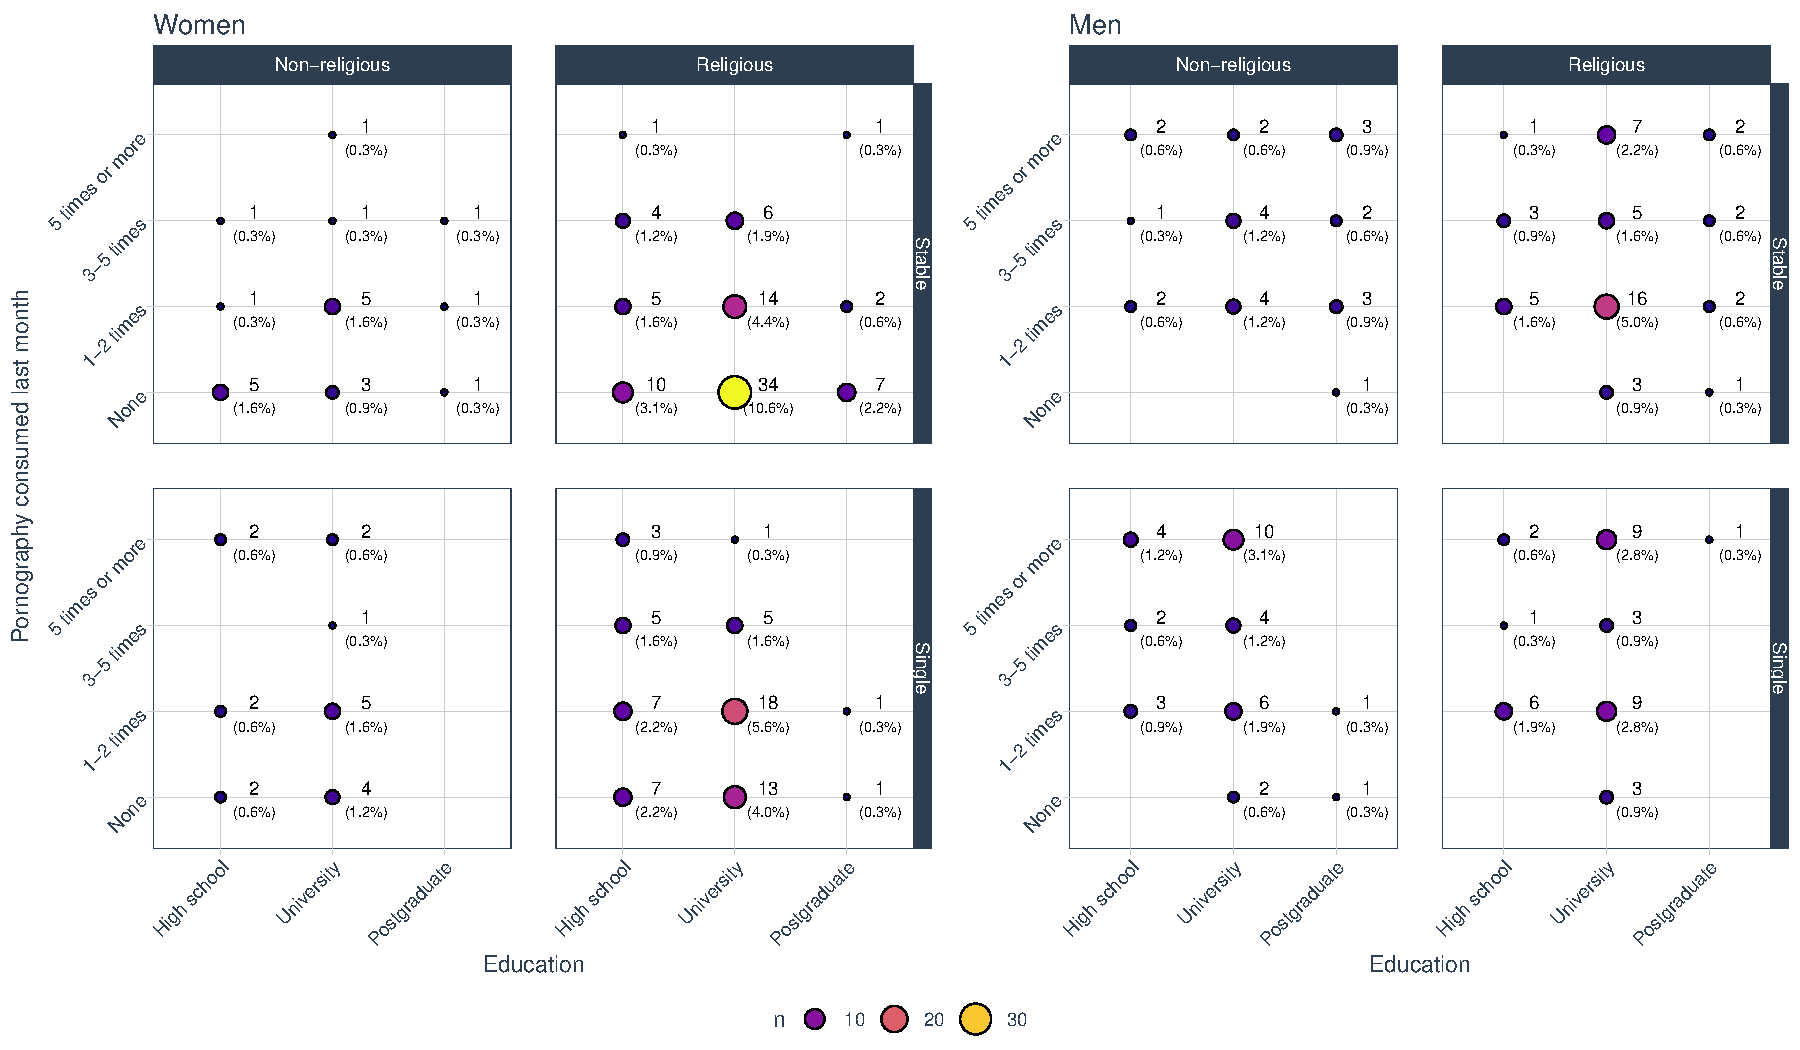
\includegraphics{Sexual_Desire_Arousal_V2_files/figure-latex/sample-plot-1.pdf}
\caption{\label{fig:sample-plot}Number of participants by gender (left = women, rigth = men), Relationship (stable = top panels, single = bottom panels), Religion (non-religious = left panels by gender, religious = right panels by gender), Education (\emph{X} axis), and pornography consumed during the last month (\emph{Y} axis). The number of participants for each combination of these five variables is displayed as numbers (percentage in brackets), as well as by the color and size of the bubbles .}
\end{figure}

\subsection{Descriptive statistics of the participants by gender}\label{descriptive-statistics-of-the-participants-by-gender}

Calculate mean values per participant for relevant, numeric variables.

\begin{Shaded}
\begin{Highlighting}[]
\CommentTok{\# Summarize relevant variables by participant}
\NormalTok{dat.desc }\OtherTok{\textless{}{-}}\NormalTok{ dat }\SpecialCharTok{|\textgreater{}}
  \FunctionTok{select}\NormalTok{(Participant, Gender, Age, Relationship, }\StringTok{\textasciigrave{}}\AttributeTok{Number of sexual partners}\StringTok{\textasciigrave{}}\NormalTok{, }
         \StringTok{\textasciigrave{}}\AttributeTok{MGH{-}SFQ (total)}\StringTok{\textasciigrave{}}\NormalTok{, }
         \StringTok{\textasciigrave{}}\AttributeTok{MGSS sexual satisfaction (General)}\StringTok{\textasciigrave{}}\NormalTok{, }\StringTok{\textasciigrave{}}\AttributeTok{MGSS sexual satisfaction (Partner)}\StringTok{\textasciigrave{}}\NormalTok{, }
         \StringTok{\textasciigrave{}}\AttributeTok{Subjective sexual attractiveness}\StringTok{\textasciigrave{}}\NormalTok{, }\StringTok{\textasciigrave{}}\AttributeTok{Subjective sexual arousal}\StringTok{\textasciigrave{}}\NormalTok{, }
         \StringTok{\textasciigrave{}}\AttributeTok{Solitary sexual desire}\StringTok{\textasciigrave{}}\NormalTok{, }
         \StringTok{\textasciigrave{}}\AttributeTok{Dyadic sexual desire (Attractive person)}\StringTok{\textasciigrave{}}\NormalTok{, }\StringTok{\textasciigrave{}}\AttributeTok{Dyadic sexual desire (Partner)}\StringTok{\textasciigrave{}}\NormalTok{) }\SpecialCharTok{|\textgreater{}}
  \FunctionTok{group\_by}\NormalTok{(Participant, Gender, Relationship) }\SpecialCharTok{|\textgreater{}}
  \FunctionTok{summarize\_if}\NormalTok{(is.numeric, mean, }\AttributeTok{na.rm =} \ConstantTok{TRUE}\NormalTok{)}
\end{Highlighting}
\end{Shaded}

\subsubsection{Table \ref{tab:desciptive-tab}. Descriptive statistics of the participants by gender}\label{table-reftabdesciptive-tab.-descriptive-statistics-of-the-participants-by-gender}

Table of descriptives by gender.

\begin{Shaded}
\begin{Highlighting}[]
\CommentTok{\# Table of descriptives by gender and relationship status}
\FunctionTok{describeBy}\NormalTok{(dat.desc }\SpecialCharTok{\textasciitilde{}}\NormalTok{ Relationship }\SpecialCharTok{+}\NormalTok{ Gender,}
           \AttributeTok{mat=}\ConstantTok{TRUE}\NormalTok{,}
           \AttributeTok{digits=}\DecValTok{2}\NormalTok{)  }\SpecialCharTok{|\textgreater{}} 
  \FunctionTok{rownames\_to\_column}\NormalTok{(}\StringTok{"Measured characteristic"}\NormalTok{) }\SpecialCharTok{|\textgreater{}}
  \FunctionTok{select}\NormalTok{(}\DecValTok{1}\NormalTok{,}\DecValTok{3}\SpecialCharTok{:}\DecValTok{4}\NormalTok{,}\DecValTok{6}\SpecialCharTok{:}\DecValTok{9}\NormalTok{,}\DecValTok{12}\SpecialCharTok{:}\DecValTok{13}\NormalTok{) }\SpecialCharTok{|\textgreater{}} 
  \FunctionTok{slice}\NormalTok{(}\SpecialCharTok{{-}}\NormalTok{(}\DecValTok{1}\SpecialCharTok{:}\DecValTok{12}\NormalTok{)) }\SpecialCharTok{|\textgreater{}} 
  \FunctionTok{select}\NormalTok{(}\DecValTok{1}\NormalTok{,}\DecValTok{3}\NormalTok{,}\DecValTok{2}\NormalTok{,}\DecValTok{4}\SpecialCharTok{:}\DecValTok{9}\NormalTok{) }\SpecialCharTok{|\textgreater{}} 
  \CommentTok{\# Remove numbers included to differentiate repeated row names (now on column 1)}
  \FunctionTok{mutate}\NormalTok{(}\StringTok{"Measured characteristic"} \OtherTok{=} \FunctionTok{str\_replace\_all}\NormalTok{(}\StringTok{\textasciigrave{}}\AttributeTok{Measured characteristic}\StringTok{\textasciigrave{}}\NormalTok{,}
                                                     \FunctionTok{c}\NormalTok{(}\StringTok{"1"} \OtherTok{=} \StringTok{""}\NormalTok{, }\StringTok{"2"} \OtherTok{=} \StringTok{""}\NormalTok{, }\StringTok{"3"} \OtherTok{=} \StringTok{""}\NormalTok{, }\StringTok{"4"} \OtherTok{=} \StringTok{""}\NormalTok{))) }\SpecialCharTok{|\textgreater{}} 
  \CommentTok{\# Create table}
  \FunctionTok{kable}\NormalTok{(}\AttributeTok{digits =} \DecValTok{2}\NormalTok{,}
        \AttributeTok{booktabs =} \ConstantTok{TRUE}\NormalTok{,}
        \AttributeTok{align =} \FunctionTok{c}\NormalTok{(}\StringTok{"l"}\NormalTok{, }\StringTok{"l"}\NormalTok{, }\FunctionTok{rep}\NormalTok{(}\StringTok{"c"}\NormalTok{, }\DecValTok{7}\NormalTok{)),}
        \AttributeTok{linesep =} \StringTok{""}\NormalTok{,}
        \AttributeTok{caption =} \StringTok{"Descriptive statistics the participants by gender}
\StringTok{        and relationship status"}\NormalTok{,}
        \AttributeTok{col.names =} \FunctionTok{c}\NormalTok{(}\StringTok{"Measured characteristic"}\NormalTok{, }\StringTok{"Gender"}\NormalTok{, }\StringTok{"Relationship status"}\NormalTok{,}
                      \StringTok{"$n$"}\NormalTok{, }\StringTok{"Mean"}\NormalTok{, }\StringTok{"$SD$"}\NormalTok{, }\StringTok{"Median"}\NormalTok{, }\StringTok{"Min"}\NormalTok{, }\StringTok{"Max"}\NormalTok{),}
        \AttributeTok{longtable =} \ConstantTok{TRUE}\NormalTok{,}
        \AttributeTok{escape =} \ConstantTok{FALSE}\NormalTok{) }\SpecialCharTok{|\textgreater{}}
  \FunctionTok{kable\_styling}\NormalTok{(}\AttributeTok{latex\_options =} \FunctionTok{c}\NormalTok{(}\StringTok{"HOLD\_position"}\NormalTok{),}
                \AttributeTok{font\_size =} \FloatTok{8.2}\NormalTok{) }\SpecialCharTok{|\textgreater{}}
  \FunctionTok{collapse\_rows}\NormalTok{(}\AttributeTok{columns =} \DecValTok{1}\SpecialCharTok{:}\DecValTok{3}\NormalTok{, }\AttributeTok{valign =} \StringTok{"middle"}\NormalTok{) }\SpecialCharTok{|\textgreater{}} 
  \FunctionTok{footnote}\NormalTok{(}\AttributeTok{general =} \StringTok{"Because for }\SpecialCharTok{\textbackslash{}\textbackslash{}\textbackslash{}\textbackslash{}}\StringTok{textit\{Subjective sexual attractiveness\} and }
\StringTok{           }\SpecialCharTok{\textbackslash{}\textbackslash{}\textbackslash{}\textbackslash{}}\StringTok{textit\{Subjective sexual arousal\} there are are multiple within{-}subject }
\StringTok{           observations, descriptives are calculated from mean values per participant."}\NormalTok{,}
           \AttributeTok{threeparttable =} \ConstantTok{TRUE}\NormalTok{,}
           \AttributeTok{footnote\_as\_chunk =} \ConstantTok{TRUE}\NormalTok{,}
           \AttributeTok{escape =} \ConstantTok{FALSE}\NormalTok{)}
\end{Highlighting}
\end{Shaded}

\begingroup\fontsize{8.2}{10.2}\selectfont

\begin{ThreePartTable}
\begin{TableNotes}[para]
\item \textit{Note: } 
\item Because for \textit{Subjective sexual attractiveness} and 
           \textit{Subjective sexual arousal} there are are multiple within-subject 
           observations, descriptives are calculated from mean values per participant.
\end{TableNotes}
\begin{longtable}[t]{llccccccc}
\caption{\label{tab:desciptive-tab}Descriptive statistics the participants by gender
        and relationship status}\\
\toprule
Measured characteristic & Gender & Relationship status & $n$ & Mean & $SD$ & Median & Min & Max\\
\midrule
 &  & Stable & 105 & 24.51 & 5.58 & 23.00 & 18.00 & 40.00\\
\cmidrule{3-9}\nopagebreak
 & \multirow{-2}{*}[0.5\dimexpr\aboverulesep+\belowrulesep+\cmidrulewidth]{\raggedright\arraybackslash Women} & Single & 79 & 22.27 & 3.84 & 21.00 & 18.00 & 36.00\\
\cmidrule{2-9}\nopagebreak
 &  & Stable & 72 & 26.72 & 5.64 & 25.00 & 19.00 & 40.00\\
\cmidrule{3-9}\nopagebreak
\multirow{-4}{*}[1.5\dimexpr\aboverulesep+\belowrulesep+\cmidrulewidth]{\raggedright\arraybackslash Age} & \multirow{-2}{*}[0.5\dimexpr\aboverulesep+\belowrulesep+\cmidrulewidth]{\raggedright\arraybackslash Men} & Single & 67 & 24.24 & 4.58 & 23.00 & 18.00 & 39.00\\
\cmidrule{1-9}\pagebreak[0]
 &  & Stable & 103 & 4.41 & 3.77 & 3.00 & 1.00 & 22.00\\
\cmidrule{3-9}\nopagebreak
 & \multirow{-2}{*}[0.5\dimexpr\aboverulesep+\belowrulesep+\cmidrulewidth]{\raggedright\arraybackslash Women} & Single & 76 & 5.74 & 8.85 & 3.00 & 0.00 & 63.00\\
\cmidrule{2-9}\nopagebreak
 &  & Stable & 72 & 8.72 & 11.36 & 5.00 & 1.00 & 70.00\\
\cmidrule{3-9}\nopagebreak
\multirow{-4}{*}[1.5\dimexpr\aboverulesep+\belowrulesep+\cmidrulewidth]{\raggedright\arraybackslash Number of sexual partners} & \multirow{-2}{*}[0.5\dimexpr\aboverulesep+\belowrulesep+\cmidrulewidth]{\raggedright\arraybackslash Men} & Single & 66 & 7.30 & 8.06 & 4.00 & 0.00 & 40.00\\
\cmidrule{1-9}\pagebreak[0]
 &  & Stable & 104 & 3.31 & 0.96 & 3.75 & 0.00 & 4.00\\
\cmidrule{3-9}\nopagebreak
 & \multirow{-2}{*}[0.5\dimexpr\aboverulesep+\belowrulesep+\cmidrulewidth]{\raggedright\arraybackslash Women} & Single & 79 & 2.80 & 1.23 & 3.50 & 0.00 & 4.00\\
\cmidrule{2-9}\nopagebreak
 &  & Stable & 72 & 3.59 & 0.62 & 3.90 & 0.60 & 4.00\\
\cmidrule{3-9}\nopagebreak
\multirow{-4}{*}[1.5\dimexpr\aboverulesep+\belowrulesep+\cmidrulewidth]{\raggedright\arraybackslash MGH-SFQ (total)} & \multirow{-2}{*}[0.5\dimexpr\aboverulesep+\belowrulesep+\cmidrulewidth]{\raggedright\arraybackslash Men} & Single & 67 & 3.38 & 0.83 & 3.80 & 0.60 & 4.00\\
\cmidrule{1-9}\pagebreak[0]
 &  & Stable & 100 & 25.88 & 5.67 & 28.00 & 6.00 & 30.00\\
\cmidrule{3-9}\nopagebreak
 & \multirow{-2}{*}[0.5\dimexpr\aboverulesep+\belowrulesep+\cmidrulewidth]{\raggedright\arraybackslash Women} & Single & 10 & 26.90 & 3.11 & 27.00 & 22.00 & 30.00\\
\cmidrule{2-9}\nopagebreak
 &  & Stable & 70 & 26.43 & 4.54 & 29.00 & 12.00 & 30.00\\
\cmidrule{3-9}\nopagebreak
\multirow{-4}{*}[1.5\dimexpr\aboverulesep+\belowrulesep+\cmidrulewidth]{\raggedright\arraybackslash MGSS sexual satisfaction (General)} & \multirow{-2}{*}[0.5\dimexpr\aboverulesep+\belowrulesep+\cmidrulewidth]{\raggedright\arraybackslash Men} & Single & 12 & 23.58 & 5.14 & 24.50 & 14.00 & 29.00\\
\cmidrule{1-9}\pagebreak[0]
 &  & Stable & 100 & 28.13 & 4.20 & 30.00 & 8.00 & 30.00\\
\cmidrule{3-9}\nopagebreak
 & \multirow{-2}{*}[0.5\dimexpr\aboverulesep+\belowrulesep+\cmidrulewidth]{\raggedright\arraybackslash Women} & Single & 10 & 28.10 & 2.13 & 29.00 & 25.00 & 30.00\\
\cmidrule{2-9}\nopagebreak
 &  & Stable & 70 & 28.49 & 3.48 & 30.00 & 6.00 & 30.00\\
\cmidrule{3-9}\nopagebreak
\multirow{-4}{*}[1.5\dimexpr\aboverulesep+\belowrulesep+\cmidrulewidth]{\raggedright\arraybackslash MGSS sexual satisfaction (Partner)} & \multirow{-2}{*}[0.5\dimexpr\aboverulesep+\belowrulesep+\cmidrulewidth]{\raggedright\arraybackslash Men} & Single & 12 & 26.08 & 4.85 & 27.50 & 15.00 & 30.00\\
\cmidrule{1-9}\pagebreak[0]
 &  & Stable & 105 & 2.94 & 1.11 & 2.78 & 1.00 & 5.49\\
\cmidrule{3-9}\nopagebreak
 & \multirow{-2}{*}[0.5\dimexpr\aboverulesep+\belowrulesep+\cmidrulewidth]{\raggedright\arraybackslash Women} & Single & 79 & 3.19 & 1.06 & 3.11 & 1.44 & 6.77\\
\cmidrule{2-9}\nopagebreak
 &  & Stable & 72 & 3.27 & 0.94 & 3.24 & 1.11 & 6.20\\
\cmidrule{3-9}\nopagebreak
\multirow{-4}{*}[1.5\dimexpr\aboverulesep+\belowrulesep+\cmidrulewidth]{\raggedright\arraybackslash Subjective sexual attractiveness} & \multirow{-2}{*}[0.5\dimexpr\aboverulesep+\belowrulesep+\cmidrulewidth]{\raggedright\arraybackslash Men} & Single & 67 & 3.20 & 0.90 & 3.18 & 1.09 & 5.72\\
\cmidrule{1-9}\pagebreak[0]
 &  & Stable & 105 & 1.59 & 0.68 & 1.39 & 1.00 & 4.21\\
\cmidrule{3-9}\nopagebreak
 & \multirow{-2}{*}[0.5\dimexpr\aboverulesep+\belowrulesep+\cmidrulewidth]{\raggedright\arraybackslash Women} & Single & 79 & 1.75 & 0.71 & 1.52 & 1.00 & 4.39\\
\cmidrule{2-9}\nopagebreak
 &  & Stable & 72 & 2.24 & 0.83 & 2.07 & 1.00 & 4.57\\
\cmidrule{3-9}\nopagebreak
\multirow{-4}{*}[1.5\dimexpr\aboverulesep+\belowrulesep+\cmidrulewidth]{\raggedright\arraybackslash Subjective sexual arousal} & \multirow{-2}{*}[0.5\dimexpr\aboverulesep+\belowrulesep+\cmidrulewidth]{\raggedright\arraybackslash Men} & Single & 67 & 2.16 & 0.78 & 2.05 & 1.00 & 4.09\\
\cmidrule{1-9}\pagebreak[0]
 &  & Stable & 105 & 11.53 & 8.59 & 12.00 & 0.00 & 29.00\\
\cmidrule{3-9}\nopagebreak
 & \multirow{-2}{*}[0.5\dimexpr\aboverulesep+\belowrulesep+\cmidrulewidth]{\raggedright\arraybackslash Women} & Single & 79 & 16.03 & 8.35 & 17.00 & 0.00 & 31.00\\
\cmidrule{2-9}\nopagebreak
 &  & Stable & 72 & 17.47 & 7.51 & 17.50 & 0.00 & 31.00\\
\cmidrule{3-9}\nopagebreak
\multirow{-4}{*}[1.5\dimexpr\aboverulesep+\belowrulesep+\cmidrulewidth]{\raggedright\arraybackslash Solitary sexual desire} & \multirow{-2}{*}[0.5\dimexpr\aboverulesep+\belowrulesep+\cmidrulewidth]{\raggedright\arraybackslash Men} & Single & 67 & 18.25 & 7.10 & 19.00 & 1.00 & 31.00\\
\cmidrule{1-9}\pagebreak[0]
 &  & Stable & 105 & 10.55 & 7.64 & 10.00 & 0.00 & 30.00\\
\cmidrule{3-9}\nopagebreak
 & \multirow{-2}{*}[0.5\dimexpr\aboverulesep+\belowrulesep+\cmidrulewidth]{\raggedright\arraybackslash Women} & Single & 79 & 14.06 & 7.39 & 15.00 & 0.00 & 32.00\\
\cmidrule{2-9}\nopagebreak
 &  & Stable & 72 & 16.21 & 7.44 & 15.50 & 0.00 & 32.00\\
\cmidrule{3-9}\nopagebreak
\multirow{-4}{*}[1.5\dimexpr\aboverulesep+\belowrulesep+\cmidrulewidth]{\raggedright\arraybackslash Dyadic sexual desire (Attractive person)} & \multirow{-2}{*}[0.5\dimexpr\aboverulesep+\belowrulesep+\cmidrulewidth]{\raggedright\arraybackslash Men} & Single & 67 & 17.57 & 6.66 & 17.00 & 2.00 & 30.00\\
\cmidrule{1-9}\pagebreak[0]
 &  & Stable & 105 & 27.53 & 8.50 & 30.00 & 0.00 & 38.00\\
\cmidrule{3-9}\nopagebreak
 & \multirow{-2}{*}[0.5\dimexpr\aboverulesep+\belowrulesep+\cmidrulewidth]{\raggedright\arraybackslash Women} & Single & 76 & 21.33 & 10.91 & 23.00 & 0.00 & 38.00\\
\cmidrule{2-9}\nopagebreak
 &  & Stable & 72 & 31.35 & 5.33 & 32.00 & 15.00 & 38.00\\
\cmidrule{3-9}\nopagebreak
\multirow{-4}{*}[1.5\dimexpr\aboverulesep+\belowrulesep+\cmidrulewidth]{\raggedright\arraybackslash Dyadic sexual desire (Partner)} & \multirow{-2}{*}[0.5\dimexpr\aboverulesep+\belowrulesep+\cmidrulewidth]{\raggedright\arraybackslash Men} & Single & 67 & 25.81 & 9.40 & 28.00 & 0.00 & 38.00\\
\bottomrule
\insertTableNotes
\end{longtable}
\end{ThreePartTable}
\endgroup{}

\subsubsection{Figure \ref{fig:density-plot}. Distribution of participants' measured variables by gender}\label{figure-reffigdensity-plot.-distribution-of-participants-measured-variables-by-gender}

Kernel density distributions by gender.

\begin{Shaded}
\begin{Highlighting}[]
\CommentTok{\# Convert dat.desc to long format}
\NormalTok{datp }\OtherTok{\textless{}{-}}\NormalTok{ dat.desc }\SpecialCharTok{|\textgreater{}} 
  \FunctionTok{pivot\_longer}\NormalTok{(}\AttributeTok{cols =}\NormalTok{ Age}\SpecialCharTok{:}\StringTok{\textasciigrave{}}\AttributeTok{Dyadic sexual desire (Partner)}\StringTok{\textasciigrave{}}\NormalTok{,}
               \AttributeTok{names\_to =} \StringTok{"Variable"}\NormalTok{, }
               \AttributeTok{values\_to =} \StringTok{"Value"}\NormalTok{) }\SpecialCharTok{|\textgreater{}}
  \FunctionTok{mutate}\NormalTok{(}\AttributeTok{Variable =} \FunctionTok{str\_wrap}\NormalTok{(Variable, }\AttributeTok{width =} \DecValTok{30}\NormalTok{))}

\CommentTok{\# Figure created as 3 separate panels (to use a different number of panels per row)}
\NormalTok{fs2a }\OtherTok{\textless{}{-}} \FunctionTok{ggplot}\NormalTok{(datp }\SpecialCharTok{|\textgreater{}}
                 \FunctionTok{filter}\NormalTok{(Variable }\SpecialCharTok{\%in\%} \FunctionTok{c}\NormalTok{(}\StringTok{"Age"}\NormalTok{,}
                                      \StringTok{"Number of sexual partners"}\NormalTok{,}
                                      \StringTok{"Subjective sexual}\SpecialCharTok{\textbackslash{}n}\StringTok{attractiveness"}\NormalTok{,}
                                      \StringTok{"Subjective sexual arousal"}\NormalTok{)),}
             \FunctionTok{aes}\NormalTok{(Value,}
                 \AttributeTok{fill =}\NormalTok{ Gender,}
                 \AttributeTok{colour =}\NormalTok{ Gender)) }\SpecialCharTok{+}
        \FunctionTok{geom\_density}\NormalTok{(}\AttributeTok{alpha =} \FloatTok{0.3}\NormalTok{) }\SpecialCharTok{+}
        \FunctionTok{geom\_vline}\NormalTok{(}\AttributeTok{data =}\NormalTok{ datp }\SpecialCharTok{|\textgreater{}}
                     \FunctionTok{filter}\NormalTok{(Variable }\SpecialCharTok{\%in\%} \FunctionTok{c}\NormalTok{(}\StringTok{"Age"}\NormalTok{,}
                                            \StringTok{"Number of sexual partners"}\NormalTok{,}
                                            \StringTok{"Subjective sexual}\SpecialCharTok{\textbackslash{}n}\StringTok{attractiveness"}\NormalTok{,}
                                            \StringTok{"Subjective sexual arousal"}\NormalTok{)) }\SpecialCharTok{|\textgreater{}} 
                     \FunctionTok{group\_by}\NormalTok{(Variable, Gender) }\SpecialCharTok{|\textgreater{}}
                     \FunctionTok{summarise}\NormalTok{(}\AttributeTok{mean =} \FunctionTok{mean}\NormalTok{(Value, }\AttributeTok{na.rm =}\ConstantTok{TRUE}\NormalTok{)),}
                   \AttributeTok{size =} \DecValTok{1}\NormalTok{,}
                   \FunctionTok{aes}\NormalTok{(}\AttributeTok{xintercept =}\NormalTok{ mean, }\AttributeTok{color =}\NormalTok{ Gender, }\AttributeTok{linetype =}\NormalTok{ Gender)) }\SpecialCharTok{+}
        \FunctionTok{scale\_color\_manual}\NormalTok{(}\AttributeTok{values =}\NormalTok{ color.Gender) }\SpecialCharTok{+}
        \FunctionTok{scale\_fill\_manual}\NormalTok{(}\AttributeTok{values =}\NormalTok{ color.Gender) }\SpecialCharTok{+}
        \FunctionTok{facet\_wrap}\NormalTok{(}\SpecialCharTok{\textasciitilde{}}\NormalTok{ Variable,}
                   \AttributeTok{scales =} \StringTok{"free"}\NormalTok{,}
                   \AttributeTok{ncol =} \DecValTok{4}\NormalTok{) }\SpecialCharTok{+}
        \FunctionTok{labs}\NormalTok{(}\AttributeTok{y =} \StringTok{"Density"}\NormalTok{,}
             \AttributeTok{x =} \ConstantTok{NULL}\NormalTok{) }\SpecialCharTok{+}
        \FunctionTok{theme\_tq}\NormalTok{()}

\NormalTok{fs2b }\OtherTok{\textless{}{-}} \FunctionTok{ggplot}\NormalTok{(datp }\SpecialCharTok{|\textgreater{}}
                 \FunctionTok{filter}\NormalTok{(Variable }\SpecialCharTok{\%in\%} \FunctionTok{c}\NormalTok{(}\StringTok{"MGH{-}SFQ (total)"}\NormalTok{,}
                                        \StringTok{"MGSS sexual satisfaction}\SpecialCharTok{\textbackslash{}n}\StringTok{(General)"}\NormalTok{,}
                                        \StringTok{"MGSS sexual satisfaction}\SpecialCharTok{\textbackslash{}n}\StringTok{(Partner)"}\NormalTok{)),}
             \FunctionTok{aes}\NormalTok{(Value,}
                 \AttributeTok{fill =}\NormalTok{ Gender,}
                 \AttributeTok{colour =}\NormalTok{ Gender)) }\SpecialCharTok{+}
        \FunctionTok{geom\_density}\NormalTok{(}\AttributeTok{alpha =} \FloatTok{0.3}\NormalTok{) }\SpecialCharTok{+}
        \FunctionTok{geom\_vline}\NormalTok{(}\AttributeTok{data =}\NormalTok{ datp }\SpecialCharTok{|\textgreater{}}
                     \FunctionTok{filter}\NormalTok{(Variable }\SpecialCharTok{\%in\%} \FunctionTok{c}\NormalTok{(}\StringTok{"MGH{-}SFQ (total)"}\NormalTok{,}
                                            \StringTok{"MGSS sexual satisfaction}\SpecialCharTok{\textbackslash{}n}\StringTok{(General)"}\NormalTok{,}
                                            \StringTok{"MGSS sexual satisfaction}\SpecialCharTok{\textbackslash{}n}\StringTok{(Partner)"}\NormalTok{)) }\SpecialCharTok{|\textgreater{}} 
                     \FunctionTok{group\_by}\NormalTok{(Variable, Gender) }\SpecialCharTok{|\textgreater{}}
                     \FunctionTok{summarise}\NormalTok{(}\AttributeTok{mean =} \FunctionTok{mean}\NormalTok{(Value, }\AttributeTok{na.rm =}\ConstantTok{TRUE}\NormalTok{)),}
                   \AttributeTok{size =} \DecValTok{1}\NormalTok{,}
                   \FunctionTok{aes}\NormalTok{(}\AttributeTok{xintercept =}\NormalTok{ mean, }\AttributeTok{color =}\NormalTok{ Gender, }\AttributeTok{linetype =}\NormalTok{ Gender)) }\SpecialCharTok{+}
        \FunctionTok{scale\_color\_manual}\NormalTok{(}\AttributeTok{values =}\NormalTok{ color.Gender) }\SpecialCharTok{+}
        \FunctionTok{scale\_fill\_manual}\NormalTok{(}\AttributeTok{values =}\NormalTok{ color.Gender) }\SpecialCharTok{+}
        \FunctionTok{facet\_wrap}\NormalTok{(}\SpecialCharTok{\textasciitilde{}}\NormalTok{ Variable,}
                   \AttributeTok{scales =} \StringTok{"free"}\NormalTok{,}
                   \AttributeTok{ncol =} \DecValTok{3}\NormalTok{) }\SpecialCharTok{+}
        \FunctionTok{labs}\NormalTok{(}\AttributeTok{y =} \StringTok{"Density"}\NormalTok{,}
             \AttributeTok{x =} \ConstantTok{NULL}\NormalTok{) }\SpecialCharTok{+}
        \FunctionTok{theme\_tq}\NormalTok{()}

\NormalTok{fs2c }\OtherTok{\textless{}{-}} \FunctionTok{ggplot}\NormalTok{(datp }\SpecialCharTok{|\textgreater{}}
                 \FunctionTok{filter}\NormalTok{(Variable }\SpecialCharTok{\%in\%} \FunctionTok{c}\NormalTok{(}\StringTok{"Solitary sexual desire"}\NormalTok{,}
                                        \StringTok{"Dyadic sexual desire}\SpecialCharTok{\textbackslash{}n}\StringTok{(Attractive person)"}\NormalTok{,}
                                        \StringTok{"Dyadic sexual desire (Partner)"}\NormalTok{)),}
             \FunctionTok{aes}\NormalTok{(Value,}
                 \AttributeTok{fill =}\NormalTok{ Gender,}
                 \AttributeTok{colour =}\NormalTok{ Gender)) }\SpecialCharTok{+}
        \FunctionTok{geom\_density}\NormalTok{(}\AttributeTok{alpha =} \FloatTok{0.3}\NormalTok{) }\SpecialCharTok{+}
        \FunctionTok{geom\_vline}\NormalTok{(}\AttributeTok{data =}\NormalTok{ datp }\SpecialCharTok{|\textgreater{}}
                     \FunctionTok{filter}\NormalTok{(Variable }\SpecialCharTok{\%in\%} \FunctionTok{c}\NormalTok{(}\StringTok{"Solitary sexual desire"}\NormalTok{,}
                                            \StringTok{"Dyadic sexual desire}\SpecialCharTok{\textbackslash{}n}\StringTok{(Attractive person)"}\NormalTok{,}
                                            \StringTok{"Dyadic sexual desire (Partner)"}\NormalTok{)) }\SpecialCharTok{|\textgreater{}} 
                     \FunctionTok{group\_by}\NormalTok{(Variable, Gender) }\SpecialCharTok{|\textgreater{}}
                     \FunctionTok{summarise}\NormalTok{(}\AttributeTok{mean =} \FunctionTok{mean}\NormalTok{(Value, }\AttributeTok{na.rm =}\ConstantTok{TRUE}\NormalTok{)),}
                   \AttributeTok{size =} \DecValTok{1}\NormalTok{,}
                   \FunctionTok{aes}\NormalTok{(}\AttributeTok{xintercept =}\NormalTok{ mean, }\AttributeTok{color =}\NormalTok{ Gender, }\AttributeTok{linetype =}\NormalTok{ Gender)) }\SpecialCharTok{+}
        \FunctionTok{scale\_color\_manual}\NormalTok{(}\AttributeTok{values =}\NormalTok{ color.Gender) }\SpecialCharTok{+}
        \FunctionTok{scale\_fill\_manual}\NormalTok{(}\AttributeTok{values =}\NormalTok{ color.Gender) }\SpecialCharTok{+}
        \FunctionTok{facet\_wrap}\NormalTok{(}\SpecialCharTok{\textasciitilde{}}\NormalTok{ Variable,}
                   \AttributeTok{scales =} \StringTok{"free"}\NormalTok{,}
                   \AttributeTok{ncol =} \DecValTok{3}\NormalTok{) }\SpecialCharTok{+}
        \FunctionTok{labs}\NormalTok{(}\AttributeTok{y =} \StringTok{"Density"}\NormalTok{,}
             \AttributeTok{x =} \ConstantTok{NULL}\NormalTok{) }\SpecialCharTok{+}
        \FunctionTok{theme\_tq}\NormalTok{()}

\CommentTok{\# Full plot}
\FunctionTok{ggarrange}\NormalTok{(fs2a, fs2b, fs2c,}
          \AttributeTok{common.legend =} \ConstantTok{TRUE}\NormalTok{,}
          \AttributeTok{legend =} \StringTok{"bottom"}\NormalTok{,}
          \AttributeTok{nrow =} \DecValTok{3}\NormalTok{)}
\end{Highlighting}
\end{Shaded}

\begin{figure}
\centering
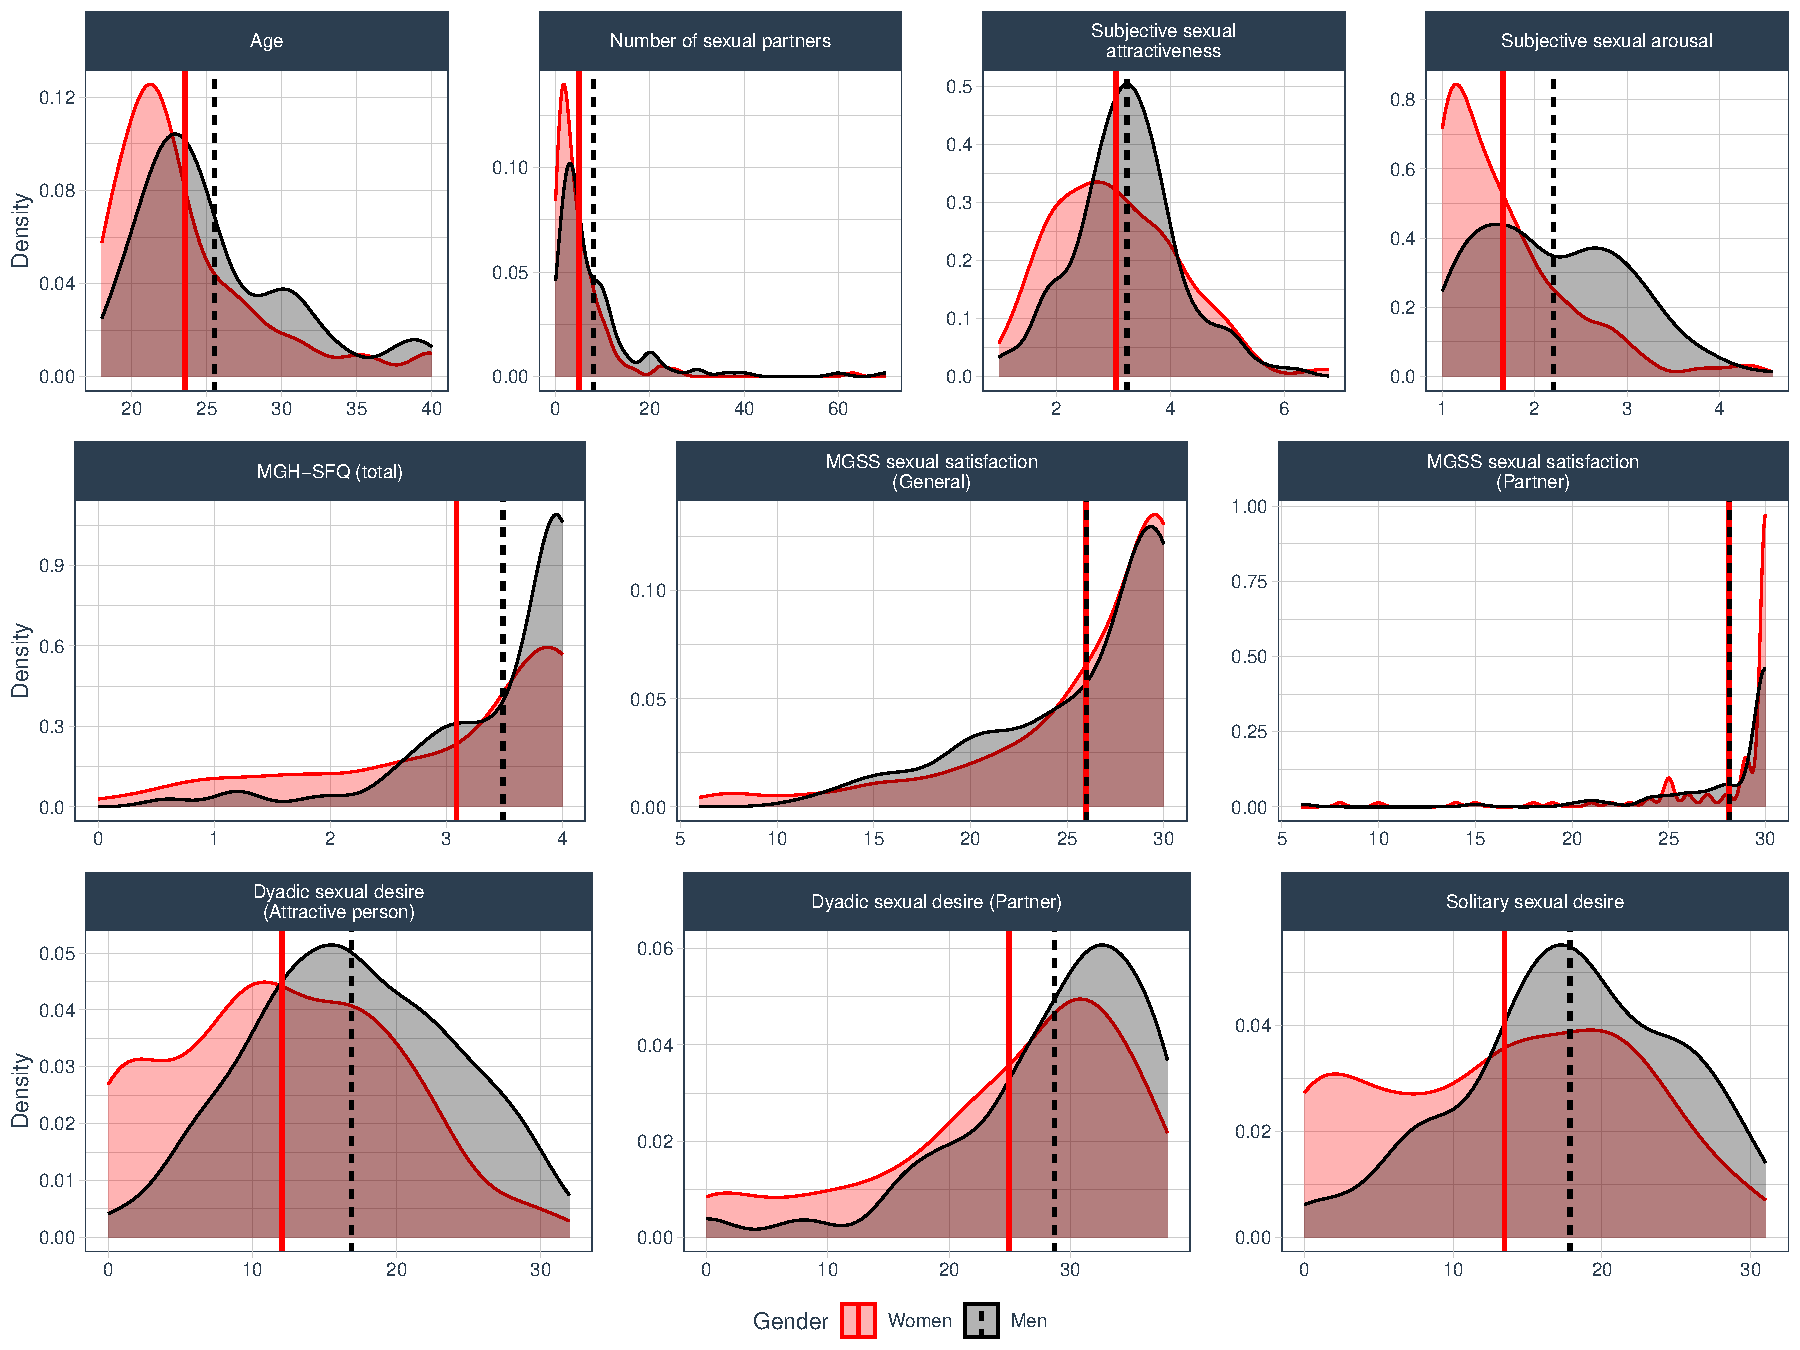
\includegraphics{Sexual_Desire_Arousal_V2_files/figure-latex/density-plot-1.pdf}
\caption{\label{fig:density-plot}Distribution of measured variables by gender. Coloured vertical lines represent mean values by gender. Detailed descriptives are found in Table S1. Because for \emph{Subjective sexual attractiveness} and \emph{Subjective sexual arousal} there are are multiple within-subject observations, densities calculated from mean values per participant.}
\end{figure}

\subsection{Correlations between measured variables}\label{correlations-between-measured-variables}

Correlation between numeric variables for women, men, and all participants combined, are reported in Table \ref{tab:corr-tab}.

\subsubsection{Table \ref{tab:corr-tab}. Correlations between measured variables}\label{table-reftabcorr-tab.-correlations-between-measured-variables}

Correlation matrix table.

\begin{Shaded}
\begin{Highlighting}[]
\CommentTok{\# Correlations for women}
\NormalTok{dat.corr.W }\OtherTok{\textless{}{-}}\NormalTok{ dat.desc }\SpecialCharTok{|\textgreater{}}
  \FunctionTok{ungroup}\NormalTok{() }\SpecialCharTok{|\textgreater{}}
  \FunctionTok{filter}\NormalTok{(Gender }\SpecialCharTok{==} \StringTok{"Women"}\NormalTok{) }\SpecialCharTok{|\textgreater{}}
  \FunctionTok{select}\NormalTok{(Age}\SpecialCharTok{:}\StringTok{\textasciigrave{}}\AttributeTok{Dyadic sexual desire (Partner)}\StringTok{\textasciigrave{}}\NormalTok{) }\SpecialCharTok{|\textgreater{}}
  \FunctionTok{corr.stars}\NormalTok{() }\SpecialCharTok{|\textgreater{}}
  \FunctionTok{rownames\_to\_column}\NormalTok{(}\AttributeTok{var =} \StringTok{" "}\NormalTok{)}

\CommentTok{\# Correlations for men}
\NormalTok{dat.corr.M }\OtherTok{\textless{}{-}}\NormalTok{ dat.desc }\SpecialCharTok{|\textgreater{}}
  \FunctionTok{ungroup}\NormalTok{() }\SpecialCharTok{|\textgreater{}}
  \FunctionTok{filter}\NormalTok{(Gender }\SpecialCharTok{==} \StringTok{"Men"}\NormalTok{) }\SpecialCharTok{|\textgreater{}}
  \FunctionTok{select}\NormalTok{(Age}\SpecialCharTok{:}\StringTok{\textasciigrave{}}\AttributeTok{Dyadic sexual desire (Partner)}\StringTok{\textasciigrave{}}\NormalTok{) }\SpecialCharTok{|\textgreater{}}
  \FunctionTok{corr.stars}\NormalTok{() }\SpecialCharTok{|\textgreater{}}
  \FunctionTok{rownames\_to\_column}\NormalTok{(}\AttributeTok{var =} \StringTok{" "}\NormalTok{)}

\CommentTok{\# Correlations for all participants combined}
\NormalTok{dat.corr.All }\OtherTok{\textless{}{-}}\NormalTok{ dat.desc }\SpecialCharTok{|\textgreater{}}
  \FunctionTok{ungroup}\NormalTok{() }\SpecialCharTok{|\textgreater{}}
  \FunctionTok{select}\NormalTok{(Age}\SpecialCharTok{:}\StringTok{\textasciigrave{}}\AttributeTok{Dyadic sexual desire (Partner)}\StringTok{\textasciigrave{}}\NormalTok{) }\SpecialCharTok{|\textgreater{}}
  \FunctionTok{corr.stars}\NormalTok{() }\SpecialCharTok{|\textgreater{}}
  \FunctionTok{rownames\_to\_column}\NormalTok{(}\AttributeTok{var =} \StringTok{" "}\NormalTok{)}

\CommentTok{\# Full formated table}
\FunctionTok{bind\_rows}\NormalTok{(dat.corr.W, dat.corr.M, dat.corr.All) }\SpecialCharTok{|\textgreater{}}
  \FunctionTok{kable}\NormalTok{(}\AttributeTok{digits =} \DecValTok{2}\NormalTok{,}
        \AttributeTok{booktabs =} \ConstantTok{TRUE}\NormalTok{,}
        \AttributeTok{align =} \FunctionTok{c}\NormalTok{(}\StringTok{"l"}\NormalTok{, }\FunctionTok{rep}\NormalTok{(}\StringTok{"c"}\NormalTok{, }\DecValTok{9}\NormalTok{)),}
        \AttributeTok{linesep =} \StringTok{""}\NormalTok{,}
        \AttributeTok{caption =} \StringTok{"Correlations between measured variables"}\NormalTok{,}
        \AttributeTok{escape =} \ConstantTok{FALSE}\NormalTok{) }\SpecialCharTok{|\textgreater{}}
  \FunctionTok{pack\_rows}\NormalTok{(}\AttributeTok{group\_label =} \StringTok{"Women"}\NormalTok{,}
            \AttributeTok{start\_row =} \DecValTok{1}\NormalTok{, }\AttributeTok{end\_row =} \DecValTok{10}\NormalTok{,}
            \AttributeTok{bold =} \ConstantTok{TRUE}\NormalTok{) }\SpecialCharTok{|\textgreater{}}
  \FunctionTok{pack\_rows}\NormalTok{(}\AttributeTok{group\_label =} \StringTok{"Men"}\NormalTok{,}
            \AttributeTok{start\_row =} \DecValTok{11}\NormalTok{, }\AttributeTok{end\_row =} \DecValTok{20}\NormalTok{,}
            \AttributeTok{hline\_before =} \ConstantTok{TRUE}\NormalTok{,}
            \AttributeTok{bold =} \ConstantTok{TRUE}\NormalTok{) }\SpecialCharTok{|\textgreater{}}
  \FunctionTok{pack\_rows}\NormalTok{(}\AttributeTok{group\_label =} \StringTok{"All participants"}\NormalTok{,}
            \AttributeTok{start\_row =} \DecValTok{21}\NormalTok{, }\AttributeTok{end\_row =} \DecValTok{30}\NormalTok{,}
            \AttributeTok{hline\_before =} \ConstantTok{TRUE}\NormalTok{,}
            \AttributeTok{bold =} \ConstantTok{TRUE}\NormalTok{) }\SpecialCharTok{|\textgreater{}}
  \FunctionTok{kable\_styling}\NormalTok{(}\AttributeTok{latex\_options =} \FunctionTok{c}\NormalTok{(}\StringTok{"HOLD\_position"}\NormalTok{, }\StringTok{"scale\_down"}\NormalTok{)) }\SpecialCharTok{|\textgreater{}}
  \FunctionTok{column\_spec}\NormalTok{(}\DecValTok{2}\SpecialCharTok{:}\DecValTok{10}\NormalTok{, }\AttributeTok{width =} \StringTok{"2.2cm"}\NormalTok{) }\SpecialCharTok{|\textgreater{}}
  \FunctionTok{footnote}\NormalTok{(}\AttributeTok{general =} \FunctionTok{paste0}\NormalTok{(}\StringTok{"Values represent Pearson correlation coefficients ($r$). "}\NormalTok{,}
                            \StringTok{"For significance, $\^{}\{}\SpecialCharTok{\textbackslash{}\textbackslash{}\textbackslash{}\textbackslash{}}\StringTok{dagger\}p$ \textless{} 0.1, *$p$ \textless{} 0.05, "}\NormalTok{,}
                            \StringTok{"**$p$ \textless{} 0.01, ***$p$ \textless{} 0.001. "}\NormalTok{,}
                            \StringTok{"Significant correlations are in bold."}\NormalTok{),}
           \AttributeTok{threeparttable =} \ConstantTok{TRUE}\NormalTok{,}
           \AttributeTok{footnote\_as\_chunk =} \ConstantTok{TRUE}\NormalTok{,}
           \AttributeTok{escape =} \ConstantTok{FALSE}\NormalTok{) }\SpecialCharTok{|\textgreater{}}
  \FunctionTok{landscape}\NormalTok{()}
\end{Highlighting}
\end{Shaded}

\begin{landscape}\begin{table}[H]
\centering
\caption{\label{tab:corr-tab}Correlations between measured variables}
\centering
\resizebox{\ifdim\width>\linewidth\linewidth\else\width\fi}{!}{
\begin{threeparttable}
\begin{tabular}[t]{l>{\centering\arraybackslash}p{2.2cm}>{\centering\arraybackslash}p{2.2cm}>{\centering\arraybackslash}p{2.2cm}>{\centering\arraybackslash}p{2.2cm}>{\centering\arraybackslash}p{2.2cm}>{\centering\arraybackslash}p{2.2cm}>{\centering\arraybackslash}p{2.2cm}>{\centering\arraybackslash}p{2.2cm}>{\centering\arraybackslash}p{2.2cm}}
\toprule
  & Age & Number of sexual partners & MGH-SFQ (total) & MGSS sexual satisfaction (General) & MGSS sexual satisfaction (Partner) & Subjective sexual attractiveness & Subjective sexual arousal & Solitary sexual desire & Dyadic sexual desire (Attractive person)\\
\midrule
\addlinespace[0.3em]
\multicolumn{10}{l}{\textbf{Women}}\\
\hspace{1em}Age &  &  &  &  &  &  &  &  \vphantom{2} & \\
\hspace{1em}Number of sexual partners & \textbf{0.24**} &  &  &  &  &  &  &  & \\
\hspace{1em}MGH-SFQ (total) & -0.05 & -0.07 &  &  &  &  &  &  & \\
\hspace{1em}MGSS sexual satisfaction (General) & \textbf{-0.21*} & 0.02 & \textbf{0.46***} &  &  &  &  &  & \\
\hspace{1em}MGSS sexual satisfaction (Partner) & -0.16$^{\dagger}$ & -0.14 & \textbf{0.32***} & \textbf{0.73***} &  &  &  &  & \\
\hspace{1em}Subjective sexual attractiveness & 0.11 & \textbf{0.18*} & -0.04 & \textbf{-0.22*} & -0.18$^{\dagger}$ &  &  &  & \\
\hspace{1em}Subjective sexual arousal & 0.00 & \textbf{0.17*} & -0.13$^{\dagger}$ & -0.18$^{\dagger}$ & -0.16$^{\dagger}$ & \textbf{0.54***} &  &  & \\
\hspace{1em}Solitary sexual desire & -0.14$^{\dagger}$ & \textbf{0.28***} & 0.05 & -0.06 & -0.18$^{\dagger}$ & \textbf{0.31***} & \textbf{0.33***} &  & \\
\hspace{1em}Dyadic sexual desire (Attractive person) & 0.06 & \textbf{0.32***} & \textbf{-0.17*} & -0.04 & -0.17$^{\dagger}$ & \textbf{0.34***} & \textbf{0.36***} & \textbf{0.44***} & \\
\hspace{1em}Dyadic sexual desire (Partner) & 0.00 & \textbf{0.21**} & \textbf{0.43***} & \textbf{0.44***} & \textbf{0.27**} & 0.13$^{\dagger}$ & 0.04 & \textbf{0.31***} & 0.13$^{\dagger}$\\
\addlinespace[0.3em]
\hline
\multicolumn{10}{l}{\textbf{Men}}\\
\hspace{1em}Age &  &  &  &  &  &  &  &  \vphantom{1} & \\
\hspace{1em}Number of sexual partners & \textbf{0.23**} &  &  &  &  &  &  &  & \\
\hspace{1em}MGH-SFQ (total) & 0.04 & 0.02 &  &  &  &  &  &  & \\
\hspace{1em}MGSS sexual satisfaction (General) & \textbf{-0.24*} & -0.08 & \textbf{0.36***} &  &  &  &  &  & \\
\hspace{1em}MGSS sexual satisfaction (Partner) & -0.13 & -0.01 & 0.10 & \textbf{0.63***} &  &  &  &  & \\
\hspace{1em}Subjective sexual attractiveness & 0.10 & -0.05 & -0.08 & -0.10 & -0.02 &  &  &  & \\
\hspace{1em}Subjective sexual arousal & \textbf{0.2*} & 0.07 & 0.05 & -0.14 & -0.09 & \textbf{0.46***} &  &  & \\
\hspace{1em}Solitary sexual desire & -0.16$^{\dagger}$ & 0.00 & 0.09 & 0.10 & 0.17 & \textbf{0.26**} & 0.11 &  & \\
\hspace{1em}Dyadic sexual desire (Attractive person) & 0.12 & \textbf{0.29***} & 0.03 & -0.13 & -0.08 & \textbf{0.25**} & \textbf{0.43***} & \textbf{0.25**} & \\
\hspace{1em}Dyadic sexual desire (Partner) & 0.11 & 0.07 & \textbf{0.36***} & \textbf{0.55***} & \textbf{0.22*} & 0.14 & \textbf{0.24**} & \textbf{0.17*} & \textbf{0.2*}\\
\addlinespace[0.3em]
\hline
\multicolumn{10}{l}{\textbf{All participants}}\\
\hspace{1em}Age &  &  &  &  &  &  &  &  & \\
\hspace{1em}Number of sexual partners & \textbf{0.26***} &  &  &  &  &  &  &  & \\
\hspace{1em}MGH-SFQ (total) & 0.02 & 0.01 &  &  &  &  &  &  & \\
\hspace{1em}MGSS sexual satisfaction (General) & \textbf{-0.22**} & -0.03 & \textbf{0.42***} &  &  &  &  &  & \\
\hspace{1em}MGSS sexual satisfaction (Partner) & \textbf{-0.14*} & -0.07 & \textbf{0.24***} & \textbf{0.69***} &  &  &  &  & \\
\hspace{1em}Subjective sexual attractiveness & \textbf{0.12*} & 0.08 & -0.03 & \textbf{-0.18*} & -0.12 &  &  &  & \\
\hspace{1em}Subjective sexual arousal & \textbf{0.15**} & \textbf{0.17**} & 0.01 & \textbf{-0.15*} & -0.12$^{\dagger}$ & \textbf{0.5***} &  &  & \\
\hspace{1em}Solitary sexual desire & -0.09 & \textbf{0.17**} & 0.11$^{\dagger}$ & 0.00 & -0.05 & \textbf{0.31***} & \textbf{0.3***} &  & \\
\hspace{1em}Dyadic sexual desire (Attractive person) & \textbf{0.14*} & \textbf{0.33***} & -0.04 & -0.07 & -0.12$^{\dagger}$ & \textbf{0.32***} & \textbf{0.45***} & \textbf{0.42***} & \\
\hspace{1em}Dyadic sexual desire (Partner) & 0.08 & \textbf{0.16**} & \textbf{0.43***} & \textbf{0.46***} & \textbf{0.25***} & \textbf{0.15**} & \textbf{0.18**} & \textbf{0.3***} & \textbf{0.21***}\\
\bottomrule
\end{tabular}
\begin{tablenotes}[para]
\item \textit{Note: } 
\item Values represent Pearson correlation coefficients ($r$). For significance, $^{\dagger}p$ < 0.1, *$p$ < 0.05, **$p$ < 0.01, ***$p$ < 0.001. Significant correlations are in bold.
\end{tablenotes}
\end{threeparttable}}
\end{table}
\end{landscape}

\subsection{Internal consistency}\label{internal-consistency}

Six variables were calculated from multiple items (1. MGH-SFQ, 2. Dyadic sexual desire (Partner), 3. Solitary sexual desire, 4. Dyadic sexual desire (Attractive person), 5. MGSS sexual satisfaction (General) and 6. MGSS sexual satisfaction (Partner)).

Data by item, for each participant, is included in the following data base, loaded as \texttt{dat.reli}:

\begin{Shaded}
\begin{Highlighting}[]
\NormalTok{dat.reli }\OtherTok{\textless{}{-}} \FunctionTok{read\_excel}\NormalTok{(}\StringTok{"Data/BD\_ConsistenciaInterna.xlsx"}\NormalTok{)  }\SpecialCharTok{|\textgreater{}}  
  \FunctionTok{mutate}\NormalTok{(}\AttributeTok{Sex =} \FunctionTok{recode\_factor}\NormalTok{(Sex,}
                             \StringTok{"2"} \OtherTok{=} \StringTok{"Women"}\NormalTok{,}
                             \StringTok{"1"} \OtherTok{=} \StringTok{"Men"}\NormalTok{)) }\SpecialCharTok{|\textgreater{}} 
  \FunctionTok{rename}\NormalTok{(}\AttributeTok{Gender =}\NormalTok{ Sex) }\SpecialCharTok{|\textgreater{}} 
  \FunctionTok{filter}\NormalTok{(Participante }\SpecialCharTok{!=} \DecValTok{122}\NormalTok{)}
\end{Highlighting}
\end{Shaded}

Participant 122 was excluded because they did not respond the psychological scales.

To measure the internal consistency of these tests, we used standardized Cronbach's alpha (\(\alpha\) or Tau-equivalent reliability: \(\rho_{T}\)) coefficients, using the function \texttt{cronbach.alpha} from the package \texttt{ltm} \autocite{LtmPackageLatent2006}.

Importantly, given that for MGH-SFQ one item was answered only by men, the internal consistency of this variable was measured independently for each gender.

\begin{Shaded}
\begin{Highlighting}[]
\CommentTok{\# MGH{-}SFQ for men}
\NormalTok{MGH.m }\OtherTok{\textless{}{-}}\NormalTok{ dat.reli }\SpecialCharTok{|\textgreater{}}
  \FunctionTok{filter}\NormalTok{(Gender }\SpecialCharTok{==} \StringTok{"Men"}\NormalTok{ ) }\SpecialCharTok{|\textgreater{}} 
  \FunctionTok{select}\NormalTok{(}\DecValTok{3}\SpecialCharTok{:}\DecValTok{7}\NormalTok{) }\SpecialCharTok{|\textgreater{}} 
  \FunctionTok{drop\_na}\NormalTok{() }\SpecialCharTok{|\textgreater{}}  
  \FunctionTok{cronbach.alpha}\NormalTok{(}\AttributeTok{CI =} \ConstantTok{TRUE}\NormalTok{, }\AttributeTok{standardized =} \ConstantTok{TRUE}\NormalTok{)}

\CommentTok{\# MGH{-}SFQ for women}
\NormalTok{MGH.w }\OtherTok{\textless{}{-}}\NormalTok{ dat.reli }\SpecialCharTok{|\textgreater{}}
  \FunctionTok{filter}\NormalTok{(Gender }\SpecialCharTok{==} \StringTok{"Women"}\NormalTok{ ) }\SpecialCharTok{|\textgreater{}} 
  \FunctionTok{select}\NormalTok{(}\DecValTok{3}\SpecialCharTok{:}\DecValTok{5}\NormalTok{,}\DecValTok{7}\NormalTok{) }\SpecialCharTok{|\textgreater{}} 
  \FunctionTok{drop\_na}\NormalTok{() }\SpecialCharTok{|\textgreater{}} 
  \FunctionTok{cronbach.alpha}\NormalTok{(}\AttributeTok{CI =} \ConstantTok{TRUE}\NormalTok{, }\AttributeTok{standardized =} \ConstantTok{TRUE}\NormalTok{)}

\CommentTok{\# Dyadic sexual desire (Partner)}
\NormalTok{DSD.p }\OtherTok{\textless{}{-}}\NormalTok{ dat.reli }\SpecialCharTok{|\textgreater{}}
  \FunctionTok{select}\NormalTok{(}\DecValTok{9}\SpecialCharTok{:}\DecValTok{13}\NormalTok{) }\SpecialCharTok{|\textgreater{}} 
  \FunctionTok{drop\_na}\NormalTok{() }\SpecialCharTok{|\textgreater{}} 
  \FunctionTok{cronbach.alpha}\NormalTok{(}\AttributeTok{CI =} \ConstantTok{TRUE}\NormalTok{, }\AttributeTok{standardized =} \ConstantTok{TRUE}\NormalTok{)}

\CommentTok{\# Solitary sexual desire}
\NormalTok{SSD.p }\OtherTok{\textless{}{-}}\NormalTok{ dat.reli }\SpecialCharTok{|\textgreater{}}
  \FunctionTok{select}\NormalTok{(}\DecValTok{15}\SpecialCharTok{:}\DecValTok{18}\NormalTok{) }\SpecialCharTok{|\textgreater{}} 
  \FunctionTok{drop\_na}\NormalTok{() }\SpecialCharTok{|\textgreater{}} 
  \FunctionTok{cronbach.alpha}\NormalTok{(}\AttributeTok{CI =} \ConstantTok{TRUE}\NormalTok{, }\AttributeTok{standardized =} \ConstantTok{TRUE}\NormalTok{)}

\CommentTok{\# Dyadic sexual desire (Attractive person)}
\NormalTok{DSD.a }\OtherTok{\textless{}{-}}\NormalTok{ dat.reli }\SpecialCharTok{|\textgreater{}}
  \FunctionTok{select}\NormalTok{(}\DecValTok{20}\SpecialCharTok{:}\DecValTok{23}\NormalTok{) }\SpecialCharTok{|\textgreater{}} 
  \FunctionTok{drop\_na}\NormalTok{()}\SpecialCharTok{|\textgreater{}} 
  \FunctionTok{cronbach.alpha}\NormalTok{(}\AttributeTok{CI =} \ConstantTok{TRUE}\NormalTok{, }\AttributeTok{standardized =} \ConstantTok{TRUE}\NormalTok{)}

\CommentTok{\# MGSS sexual satisfaction (General)}
\NormalTok{MGSS.g }\OtherTok{\textless{}{-}}\NormalTok{ dat.reli }\SpecialCharTok{|\textgreater{}}
  \FunctionTok{select}\NormalTok{(}\DecValTok{26}\SpecialCharTok{:}\DecValTok{30}\NormalTok{) }\SpecialCharTok{|\textgreater{}} 
  \FunctionTok{drop\_na}\NormalTok{()}\SpecialCharTok{|\textgreater{}} 
  \FunctionTok{cronbach.alpha}\NormalTok{(}\AttributeTok{CI =} \ConstantTok{TRUE}\NormalTok{, }\AttributeTok{standardized =} \ConstantTok{TRUE}\NormalTok{)}

\CommentTok{\# MGSS sexual satisfaction (Partner)}
\NormalTok{MGSS.p }\OtherTok{\textless{}{-}}\NormalTok{ dat.reli }\SpecialCharTok{|\textgreater{}}
  \FunctionTok{select}\NormalTok{(}\DecValTok{32}\SpecialCharTok{:}\DecValTok{36}\NormalTok{) }\SpecialCharTok{|\textgreater{}} 
  \FunctionTok{drop\_na}\NormalTok{()}\SpecialCharTok{|\textgreater{}} 
  \FunctionTok{cronbach.alpha}\NormalTok{(}\AttributeTok{CI =} \ConstantTok{TRUE}\NormalTok{, }\AttributeTok{standardized =} \ConstantTok{TRUE}\NormalTok{)}
\end{Highlighting}
\end{Shaded}

\subsubsection{Table \ref{tab:Cronbach-tab}. Internal consistency of construct variables}\label{table-reftabcronbach-tab.-internal-consistency-of-construct-variables}

Table of Cronbach's \(\alpha\) for construct variables.

\begin{Shaded}
\begin{Highlighting}[]
\CommentTok{\# Create table}
\FunctionTok{tibble}\NormalTok{(}\AttributeTok{Variable =} \FunctionTok{c}\NormalTok{(}\StringTok{"MGH{-}SFQ"}\NormalTok{, }\StringTok{"MGH{-}SFQ"}\NormalTok{,}
                    \StringTok{"MGSS sexual satisfaction (General)"}\NormalTok{,}
                    \StringTok{"MGSS sexual satisfaction (Partner)"}\NormalTok{,}
                    \StringTok{"Dyadic sexual desire (Partner)"}\NormalTok{, }
                    \StringTok{"Solitary sexual desire"}\NormalTok{, }
                    \StringTok{"Dyadic sexual desire (Attractive person)"}\NormalTok{),}
       \AttributeTok{Gender =} \FunctionTok{c}\NormalTok{(}\StringTok{"Men"}\NormalTok{, }\StringTok{"Women"}\NormalTok{, }\FunctionTok{rep}\NormalTok{(}\StringTok{" "}\NormalTok{, }\DecValTok{5}\NormalTok{)),}
       \AttributeTok{p =} \FunctionTok{c}\NormalTok{(MGH.m}\SpecialCharTok{$}\NormalTok{p,}
\NormalTok{             MGH.w}\SpecialCharTok{$}\NormalTok{p,}
\NormalTok{             MGSS.g}\SpecialCharTok{$}\NormalTok{p,}
\NormalTok{             MGSS.p}\SpecialCharTok{$}\NormalTok{p,}
\NormalTok{             DSD.p}\SpecialCharTok{$}\NormalTok{p,}
\NormalTok{             SSD.p}\SpecialCharTok{$}\NormalTok{p,}
\NormalTok{             DSD.a}\SpecialCharTok{$}\NormalTok{p),}
       \AttributeTok{n =} \FunctionTok{c}\NormalTok{(MGH.m}\SpecialCharTok{$}\NormalTok{n, }
\NormalTok{             MGH.w}\SpecialCharTok{$}\NormalTok{n,}
\NormalTok{             MGSS.g}\SpecialCharTok{$}\NormalTok{n,}
\NormalTok{             MGSS.p}\SpecialCharTok{$}\NormalTok{n,}
\NormalTok{             DSD.p}\SpecialCharTok{$}\NormalTok{n,}
\NormalTok{             SSD.p}\SpecialCharTok{$}\NormalTok{n,}
\NormalTok{             DSD.a}\SpecialCharTok{$}\NormalTok{n),}
       \AttributeTok{alpha =} \FunctionTok{c}\NormalTok{(MGH.m}\SpecialCharTok{$}\NormalTok{alpha,}
\NormalTok{                 MGH.w}\SpecialCharTok{$}\NormalTok{alpha,}
\NormalTok{                 MGSS.g}\SpecialCharTok{$}\NormalTok{alpha,}
\NormalTok{                 MGSS.p}\SpecialCharTok{$}\NormalTok{alpha,}
\NormalTok{                 DSD.p}\SpecialCharTok{$}\NormalTok{alpha,}
\NormalTok{                 SSD.p}\SpecialCharTok{$}\NormalTok{alpha,}
\NormalTok{                 DSD.a}\SpecialCharTok{$}\NormalTok{alpha), }
       \AttributeTok{ci2.5 =} \FunctionTok{c}\NormalTok{(MGH.m}\SpecialCharTok{$}\NormalTok{ci[}\DecValTok{1}\NormalTok{], }
\NormalTok{                 MGH.w}\SpecialCharTok{$}\NormalTok{ci[}\DecValTok{1}\NormalTok{],}
\NormalTok{                 MGSS.g}\SpecialCharTok{$}\NormalTok{ci[}\DecValTok{1}\NormalTok{],}
\NormalTok{                 MGSS.p}\SpecialCharTok{$}\NormalTok{ci[}\DecValTok{1}\NormalTok{],}
\NormalTok{                 DSD.p}\SpecialCharTok{$}\NormalTok{ci[}\DecValTok{1}\NormalTok{],}
\NormalTok{                 SSD.p}\SpecialCharTok{$}\NormalTok{ci[}\DecValTok{1}\NormalTok{],}
\NormalTok{                 DSD.a}\SpecialCharTok{$}\NormalTok{ci[}\DecValTok{1}\NormalTok{]),}
       \AttributeTok{ci97.5 =} \FunctionTok{c}\NormalTok{(MGH.m}\SpecialCharTok{$}\NormalTok{ci[}\DecValTok{2}\NormalTok{], }
\NormalTok{                  MGH.w}\SpecialCharTok{$}\NormalTok{ci[}\DecValTok{2}\NormalTok{],}
\NormalTok{                  MGSS.g}\SpecialCharTok{$}\NormalTok{ci[}\DecValTok{2}\NormalTok{],}
\NormalTok{                  MGSS.p}\SpecialCharTok{$}\NormalTok{ci[}\DecValTok{2}\NormalTok{],}
\NormalTok{                  DSD.p}\SpecialCharTok{$}\NormalTok{ci[}\DecValTok{2}\NormalTok{],}
\NormalTok{                  SSD.p}\SpecialCharTok{$}\NormalTok{ci[}\DecValTok{2}\NormalTok{],}
\NormalTok{                  DSD.a}\SpecialCharTok{$}\NormalTok{ci[}\DecValTok{2}\NormalTok{])) }\SpecialCharTok{|\textgreater{}} 
  \FunctionTok{kable}\NormalTok{(}\AttributeTok{digits =} \DecValTok{2}\NormalTok{,}
        \AttributeTok{booktabs =} \ConstantTok{TRUE}\NormalTok{,}
        \AttributeTok{align =} \FunctionTok{c}\NormalTok{(}\StringTok{"l"}\NormalTok{, }\StringTok{"l"}\NormalTok{, }\FunctionTok{rep}\NormalTok{(}\StringTok{"c"}\NormalTok{, }\DecValTok{5}\NormalTok{)),}
        \AttributeTok{linesep =} \StringTok{""}\NormalTok{,}
        \AttributeTok{caption =} \StringTok{"Internal consistency of measured variables"}\NormalTok{,}
        \AttributeTok{escape =} \ConstantTok{FALSE}\NormalTok{,}
        \AttributeTok{col.names =} \FunctionTok{c}\NormalTok{(}\StringTok{"Variable"}\NormalTok{, }\StringTok{"Gender"}\NormalTok{,}
                      \StringTok{"Items"}\NormalTok{,}
                      \StringTok{"$n$"}\NormalTok{,}
                      \StringTok{"$}\SpecialCharTok{\textbackslash{}\textbackslash{}}\StringTok{alpha$"}\NormalTok{,}
                      \StringTok{"$2.5}\SpecialCharTok{\textbackslash{}\textbackslash{}}\StringTok{\% CI$"}\NormalTok{,}
                      \StringTok{"$97.5}\SpecialCharTok{\textbackslash{}\textbackslash{}}\StringTok{\% CI$"}\NormalTok{)) }\SpecialCharTok{|\textgreater{}}
  \FunctionTok{collapse\_rows}\NormalTok{(}\AttributeTok{columns =} \DecValTok{1}\NormalTok{, }\AttributeTok{valign =} \StringTok{"middle"}\NormalTok{) }\SpecialCharTok{|\textgreater{}}
  \FunctionTok{kable\_styling}\NormalTok{(}\AttributeTok{latex\_options =} \StringTok{"HOLD\_position"}\NormalTok{) }\SpecialCharTok{|\textgreater{}}
  \FunctionTok{footnote}\NormalTok{(}\AttributeTok{general =} \StringTok{"95}\SpecialCharTok{\textbackslash{}\textbackslash{}\textbackslash{}\textbackslash{}}\StringTok{\% confidence intervals were calculated with 1,000 bootstrap samples.}
\StringTok{           Standardized Cronbach\textquotesingle{}s alpha ($}\SpecialCharTok{\textbackslash{}\textbackslash{}\textbackslash{}\textbackslash{}}\StringTok{alpha$) coefficients were computed. }
\StringTok{           MGH{-}SFQ is reported by gender, because one item was answered only by men."}\NormalTok{,}
           \AttributeTok{threeparttable =} \ConstantTok{TRUE}\NormalTok{,}
           \AttributeTok{footnote\_as\_chunk =} \ConstantTok{TRUE}\NormalTok{,}
           \AttributeTok{escape =} \ConstantTok{FALSE}\NormalTok{)}
\end{Highlighting}
\end{Shaded}

\begin{table}[H]
\centering
\caption{\label{tab:Cronbach-tab}Internal consistency of measured variables}
\centering
\begin{threeparttable}
\begin{tabular}[t]{llccccc}
\toprule
Variable & Gender & Items & $n$ & $\alpha$ & $2.5\% CI$ & $97.5\% CI$\\
\midrule
 & Men & 5 & 139 & 0.82 & 0.72 & 0.89\\
\cmidrule{2-7}
\multirow{-2}{*}{\raggedright\arraybackslash MGH-SFQ} & Women & 4 & 181 & 0.86 & 0.82 & 0.90\\
\cmidrule{1-7}
MGSS sexual satisfaction (General) &  & 5 & 188 & 0.92 & 0.88 & 0.94\\
\cmidrule{1-7}
MGSS sexual satisfaction (Partner) &  & 5 & 187 & 0.91 & 0.85 & 0.95\\
\cmidrule{1-7}
Dyadic sexual desire (Partner) &  & 5 & 309 & 0.90 & 0.87 & 0.92\\
\cmidrule{1-7}
Solitary sexual desire &  & 4 & 314 & 0.91 & 0.89 & 0.93\\
\cmidrule{1-7}
Dyadic sexual desire (Attractive person) &  & 4 & 320 & 0.89 & 0.87 & 0.91\\
\bottomrule
\end{tabular}
\begin{tablenotes}[para]
\item \textit{Note: } 
\item 95\% confidence intervals were calculated with 1,000 bootstrap samples.
           Standardized Cronbach's alpha ($\alpha$) coefficients were computed. 
           MGH-SFQ is reported by gender, because one item was answered only by men.
\end{tablenotes}
\end{threeparttable}
\end{table}

\begin{center}\rule{0.5\linewidth}{0.5pt}\end{center}

\subsection{Controlling for Relationship Duration and MGSS Sexual Satisfaction (Partner) in Sexual Desire Dimensions}\label{controlling-for-relationship-duration-and-mgss-sexual-satisfaction-partner-in-sexual-desire-dimensions}

To \textbf{ensure that the three sexual desire dimensions were not influenced by Relationship Duration or MGSS sexual satisfaction (Partner)}, we applied a three-step adjustment process:

\begin{enumerate}
\def\labelenumi{\arabic{enumi}.}
\tightlist
\item
  \textbf{Estimating the effects:}

  \begin{itemize}
  \tightlist
  \item
    We performed separate \textbf{linear regressions} where each sexual desire dimension was predicted by \textbf{Relationship Duration} and \textbf{MGSS sexual satisfaction (Partner)}.
  \item
    This allowed us to quantify how much these external factors influence each dimension.
  \end{itemize}
\item
  \textbf{Evaluating statistical significance:}

  \begin{itemize}
  \tightlist
  \item
    We conducted \textbf{Type III ANOVA} to determine which predictors had a significant effect on each sexual desire dimension.
  \item
    Only \textbf{MGSS sexual satisfaction (Partner) significantly predicted Dyadic Sexual Desire (Partner)}.
  \end{itemize}
\item
  \textbf{Removing the effects:}

  \begin{itemize}
  \tightlist
  \item
    We adjusted \textbf{only Dyadic Sexual Desire (Partner)} by extracting the \textbf{residuals} from the regression model.
  \item
    These residuals represent the \textbf{variation independent of MGSS sexual satisfaction (Partner)} and were then standardized for comparability.
  \end{itemize}
\end{enumerate}

Additionally, \textbf{MGSS sexual satisfaction (Partner) was mean-centered} before analysis.

\textbf{Step 1}: Estimating the Effects of Relationship Duration \& Partner Satisfaction

\begin{Shaded}
\begin{Highlighting}[]
\CommentTok{\# Select only participants in stable relationships and ensure required variables are available}
\NormalTok{dat\_ctl }\OtherTok{\textless{}{-}}\NormalTok{ dat }\SpecialCharTok{|\textgreater{}}
  \FunctionTok{group\_by}\NormalTok{(Participant) }\SpecialCharTok{|\textgreater{}}  
  \FunctionTok{slice\_head}\NormalTok{() }\SpecialCharTok{|\textgreater{}}  
  \FunctionTok{filter}\NormalTok{(Relationship }\SpecialCharTok{==} \StringTok{"Stable"}\NormalTok{) }\SpecialCharTok{|\textgreater{}}  
  \FunctionTok{ungroup}\NormalTok{()}

\CommentTok{\# Fit linear models predicting each dimension of sexual desire}
\NormalTok{ctl\_SSD }\OtherTok{\textless{}{-}} \FunctionTok{lm}\NormalTok{(}\StringTok{\textasciigrave{}}\AttributeTok{Solitary sexual desire}\StringTok{\textasciigrave{}} \SpecialCharTok{\textasciitilde{}} 
                \StringTok{\textasciigrave{}}\AttributeTok{Relationship duration}\StringTok{\textasciigrave{}} \SpecialCharTok{+} \StringTok{\textasciigrave{}}\AttributeTok{MGSS sexual satisfaction (Partner)}\StringTok{\textasciigrave{}}\NormalTok{, }
              \AttributeTok{data =}\NormalTok{ dat\_ctl)}
\NormalTok{ctl\_PD }\OtherTok{\textless{}{-}} \FunctionTok{lm}\NormalTok{(}\StringTok{\textasciigrave{}}\AttributeTok{Dyadic sexual desire (Partner)}\StringTok{\textasciigrave{}} \SpecialCharTok{\textasciitilde{}} 
               \StringTok{\textasciigrave{}}\AttributeTok{Relationship duration}\StringTok{\textasciigrave{}} \SpecialCharTok{+} \StringTok{\textasciigrave{}}\AttributeTok{MGSS sexual satisfaction (Partner)}\StringTok{\textasciigrave{}}\NormalTok{, }
             \AttributeTok{data =}\NormalTok{ dat\_ctl)}
\NormalTok{ctl\_APD }\OtherTok{\textless{}{-}} \FunctionTok{lm}\NormalTok{(}\StringTok{\textasciigrave{}}\AttributeTok{Dyadic sexual desire (Attractive person)}\StringTok{\textasciigrave{}} \SpecialCharTok{\textasciitilde{}} 
                \StringTok{\textasciigrave{}}\AttributeTok{Relationship duration}\StringTok{\textasciigrave{}} \SpecialCharTok{+} \StringTok{\textasciigrave{}}\AttributeTok{MGSS sexual satisfaction (Partner)}\StringTok{\textasciigrave{}}\NormalTok{, }
              \AttributeTok{data =}\NormalTok{ dat\_ctl)}
\end{Highlighting}
\end{Shaded}

\textbf{Step 2}: Displaying ANOVA Results for Each Model

The table below presents Type III ANOVA results for each model. Significant effects indicate that Relationship Duration or Partner Satisfaction meaningfully predict the corresponding sexual desire dimension.

\begin{Shaded}
\begin{Highlighting}[]
\CommentTok{\# Combine ANOVA results for all models}
\NormalTok{anova\_results }\OtherTok{\textless{}{-}} \FunctionTok{bind\_cols}\NormalTok{(}\FunctionTok{anova\_summary}\NormalTok{(}\FunctionTok{Anova}\NormalTok{(ctl\_SSD, }\AttributeTok{type =} \DecValTok{3}\NormalTok{)) }\SpecialCharTok{|\textgreater{}}
                             \FunctionTok{unite}\NormalTok{(}\AttributeTok{col =} \StringTok{"df"}\NormalTok{, DFn}\SpecialCharTok{:}\NormalTok{DFd, }\AttributeTok{sep =} \StringTok{", "}\NormalTok{),}
                           \FunctionTok{anova\_summary}\NormalTok{(}\FunctionTok{Anova}\NormalTok{(ctl\_PD, }\AttributeTok{type =} \DecValTok{3}\NormalTok{)) }\SpecialCharTok{|\textgreater{}}
                             \FunctionTok{unite}\NormalTok{(}\AttributeTok{col =} \StringTok{"df"}\NormalTok{, DFn}\SpecialCharTok{:}\NormalTok{DFd, }\AttributeTok{sep =} \StringTok{", "}\NormalTok{),}
                           \FunctionTok{anova\_summary}\NormalTok{(}\FunctionTok{Anova}\NormalTok{(ctl\_APD, }\AttributeTok{type =} \DecValTok{3}\NormalTok{)) }\SpecialCharTok{|\textgreater{}}
                             \FunctionTok{unite}\NormalTok{(}\AttributeTok{col =} \StringTok{"df"}\NormalTok{, DFn}\SpecialCharTok{:}\NormalTok{DFd, }\AttributeTok{sep =} \StringTok{", "}\NormalTok{)) }\SpecialCharTok{|\textgreater{}}
  \FunctionTok{select}\NormalTok{(}\SpecialCharTok{{-}}\FunctionTok{starts\_with}\NormalTok{(}\StringTok{"p\textless{}.05"}\NormalTok{)) }\SpecialCharTok{|\textgreater{}}  \CommentTok{\# Remove Sum of Squares columns}
  \FunctionTok{mutate}\NormalTok{(}\FunctionTok{across}\NormalTok{(}\FunctionTok{starts\_with}\NormalTok{(}\StringTok{"p..."}\NormalTok{), pval.lev)) }\SpecialCharTok{|\textgreater{}} \CommentTok{\# Format p{-}values}
  \FunctionTok{rename}\NormalTok{(}\AttributeTok{Effect =}\NormalTok{ Effect...}\DecValTok{1}\NormalTok{) }\SpecialCharTok{|\textgreater{}} 
  \FunctionTok{select}\NormalTok{(}\SpecialCharTok{{-}}\FunctionTok{starts\_with}\NormalTok{(}\StringTok{"Effect..."}\NormalTok{)) }\SpecialCharTok{|\textgreater{}} 
  \FunctionTok{mutate\_at}\NormalTok{(}\StringTok{"Effect"}\NormalTok{, str\_replace\_all, }\StringTok{"\textasciigrave{}"}\NormalTok{, }\StringTok{""}\NormalTok{)}

\CommentTok{\# Create a formatted table}
\NormalTok{anova\_results }\SpecialCharTok{|\textgreater{}} 
  \FunctionTok{kable}\NormalTok{(}\AttributeTok{booktabs =} \ConstantTok{TRUE}\NormalTok{,}
        \AttributeTok{align =} \FunctionTok{c}\NormalTok{(}\StringTok{"l"}\NormalTok{, }\FunctionTok{rep}\NormalTok{(}\StringTok{"c"}\NormalTok{, }\DecValTok{9}\NormalTok{)),  }\CommentTok{\# Align columns (left for first, center for the rest)}
        \AttributeTok{digits =} \DecValTok{3}\NormalTok{,}
        \AttributeTok{caption =} \StringTok{"Effects of relationship duration and MGSS sexual satisfaction (Partner) in }
\StringTok{                   sexual desire dimensions"}\NormalTok{,}
        \AttributeTok{col.names =} \FunctionTok{c}\NormalTok{(}\StringTok{"Effect"}\NormalTok{, }\FunctionTok{rep}\NormalTok{(}\FunctionTok{c}\NormalTok{(}\StringTok{"$df$"}\NormalTok{, }\StringTok{"$F$"}\NormalTok{, }\StringTok{"$p$"}\NormalTok{, }\StringTok{"$}\SpecialCharTok{\textbackslash{}\textbackslash{}}\StringTok{eta\^{}2\_G$"}\NormalTok{), }\AttributeTok{times =} \DecValTok{3}\NormalTok{)),}
        \AttributeTok{escape =} \ConstantTok{FALSE}\NormalTok{) }\SpecialCharTok{|\textgreater{}} 
  \FunctionTok{kable\_styling}\NormalTok{(}\AttributeTok{latex\_options =} \FunctionTok{c}\NormalTok{(}\StringTok{"HOLD\_position"}\NormalTok{, }\StringTok{"scale\_down"}\NormalTok{)) }\SpecialCharTok{|\textgreater{}}
  \FunctionTok{add\_header\_above}\NormalTok{(}\FunctionTok{c}\NormalTok{(}\StringTok{" "} \OtherTok{=} \DecValTok{1}\NormalTok{, }
                     \StringTok{"Solitary sexual desire"} \OtherTok{=} \DecValTok{4}\NormalTok{,}
                     \StringTok{"Dyadic sexual desire}\SpecialCharTok{\textbackslash{}n}\StringTok{(Partner)"} \OtherTok{=} \DecValTok{4}\NormalTok{,}
                     \StringTok{"Dyadic sexual desire}\SpecialCharTok{\textbackslash{}n}\StringTok{(Attractive person)"} \OtherTok{=} \DecValTok{4}\NormalTok{)) }\SpecialCharTok{|\textgreater{}}
  \FunctionTok{footnote}\NormalTok{(}\AttributeTok{general =} \StringTok{"As effect size, we used the generalized eta squared }
\StringTok{                     ($}\SpecialCharTok{\textbackslash{}\textbackslash{}\textbackslash{}\textbackslash{}}\StringTok{eta\^{}2\_G$; see}
\StringTok{                     }\SpecialCharTok{\textbackslash{}\textbackslash{}\textbackslash{}\textbackslash{}}\StringTok{cite\{bakemanRecommendedEffectSize2005\}).}
\StringTok{                     Significant effects are in bold."}\NormalTok{,}
           \AttributeTok{threeparttable =} \ConstantTok{TRUE}\NormalTok{,}
           \AttributeTok{footnote\_as\_chunk =} \ConstantTok{TRUE}\NormalTok{,}
           \AttributeTok{escape =} \ConstantTok{FALSE}\NormalTok{)}
\end{Highlighting}
\end{Shaded}

\begin{table}[H]
\centering
\caption{\label{tab:unnamed-chunk-15}Effects of relationship duration and MGSS sexual satisfaction (Partner) in 
                   sexual desire dimensions}
\centering
\resizebox{\ifdim\width>\linewidth\linewidth\else\width\fi}{!}{
\begin{threeparttable}
\begin{tabular}[t]{lccccccccclcc}
\toprule
\multicolumn{1}{c}{ } & \multicolumn{4}{c}{Solitary sexual desire} & \multicolumn{4}{c}{\makecell[c]{Dyadic sexual desire\\(Partner)}} & \multicolumn{4}{c}{\makecell[c]{Dyadic sexual desire\\(Attractive person)}} \\
\cmidrule(l{3pt}r{3pt}){2-5} \cmidrule(l{3pt}r{3pt}){6-9} \cmidrule(l{3pt}r{3pt}){10-13}
Effect & $df$ & $F$ & $p$ & $\eta^2_G$ & $df$ & $F$ & $p$ & $\eta^2_G$ & $df$ & $F$ & $p$ & $\eta^2_G$\\
\midrule
Relationship duration & 3, 165 & 0.482 & 0.70 & 0.009 & 3, 165 & 2.081 & 0.1 & 0.036 & 3, 165 & 0.095 & 0.96 & 0.002\\
MGSS sexual satisfaction (Partner) & 1, 165 & 0.029 & 0.86 & 0.000 & 1, 165 & 8.875 & \textbf{0.003} & 0.051 & 1, 165 & 0.884 & 0.35 & 0.005\\
\bottomrule
\end{tabular}
\begin{tablenotes}[para]
\item \textit{Note: } 
\item As effect size, we used the generalized eta squared 
                     ($\eta^2_G$; see
                     \cite{bakemanRecommendedEffectSize2005}).
                     Significant effects are in bold.
\end{tablenotes}
\end{threeparttable}}
\end{table}

\textbf{Step 3}: Controlling Scores Based on ANOVA Results

From the ANOVA results, only the effect of MGSS sexual satisfaction (Partner) on Dyadic sexual desire (Partner) was significant. Thus, only Dyadic Sexual Desire (Partner) scores were adjusted, while the other dimensions remained unchanged.

\begin{Shaded}
\begin{Highlighting}[]
\CommentTok{\# Prepare dataset with necessary variables, removing missing values}
\NormalTok{dat\_tl\_PD\_fin }\OtherTok{\textless{}{-}}\NormalTok{ dat\_ctl }\SpecialCharTok{|\textgreater{}}
  \FunctionTok{select}\NormalTok{(Participant, }\StringTok{\textasciigrave{}}\AttributeTok{Dyadic sexual desire (Partner)}\StringTok{\textasciigrave{}}\NormalTok{, }
         \StringTok{\textasciigrave{}}\AttributeTok{MGSS sexual satisfaction (Partner)}\StringTok{\textasciigrave{}}\NormalTok{) }\SpecialCharTok{|\textgreater{}}
  \FunctionTok{drop\_na}\NormalTok{()}

\CommentTok{\# Fit a model to predict Dyadic Sexual Desire (Partner) using partner satisfaction only}
\NormalTok{ctl\_PD\_fin }\OtherTok{\textless{}{-}} \FunctionTok{lm}\NormalTok{(}\StringTok{\textasciigrave{}}\AttributeTok{Dyadic sexual desire (Partner)}\StringTok{\textasciigrave{}} \SpecialCharTok{\textasciitilde{}} \StringTok{\textasciigrave{}}\AttributeTok{MGSS sexual satisfaction (Partner)}\StringTok{\textasciigrave{}}\NormalTok{, }
                 \AttributeTok{data =}\NormalTok{ dat\_tl\_PD\_fin)}

\CommentTok{\# Adjust the Dyadic Sexual Desire (Partner) scores by replacing them with their residuals}
\NormalTok{dat\_ctl }\OtherTok{\textless{}{-}}\NormalTok{ dat\_tl\_PD\_fin }\SpecialCharTok{|\textgreater{}}
  \FunctionTok{mutate}\NormalTok{(}\StringTok{\textasciigrave{}}\AttributeTok{Dyadic sexual desire (Partner)}\StringTok{\textasciigrave{}} \OtherTok{=} 
           \FunctionTok{mean}\NormalTok{(}\StringTok{\textasciigrave{}}\AttributeTok{Dyadic sexual desire (Partner)}\StringTok{\textasciigrave{}}\NormalTok{) }\SpecialCharTok{+} \FunctionTok{resid}\NormalTok{(ctl\_PD\_fin))}

\CommentTok{\# Update the original dataset with the adjusted scores}
\NormalTok{dat }\OtherTok{\textless{}{-}}\NormalTok{ dat }\SpecialCharTok{|\textgreater{}}
  \FunctionTok{mutate}\NormalTok{(}\StringTok{\textasciigrave{}}\AttributeTok{Dyadic sexual desire (Partner)}\StringTok{\textasciigrave{}} \OtherTok{=} \FunctionTok{as.numeric}\NormalTok{(}\StringTok{\textasciigrave{}}\AttributeTok{Dyadic sexual desire (Partner)}\StringTok{\textasciigrave{}}\NormalTok{)) }\SpecialCharTok{|\textgreater{}}
  \FunctionTok{rows\_update}\NormalTok{(dat\_ctl }\SpecialCharTok{|\textgreater{}} \FunctionTok{select}\NormalTok{(}\SpecialCharTok{{-}}\StringTok{\textasciigrave{}}\AttributeTok{MGSS sexual satisfaction (Partner)}\StringTok{\textasciigrave{}}\NormalTok{), }
              \AttributeTok{by =} \StringTok{"Participant"}\NormalTok{, }\AttributeTok{unmatched =} \StringTok{"ignore"}\NormalTok{)}
\end{Highlighting}
\end{Shaded}

\begin{center}\rule{0.5\linewidth}{0.5pt}\end{center}

\section{Hypothesis tests}\label{hypothesis-tests}

\subsection{Hypothesis 1: All dimensions of trait sexual desire (TSD) will be higher in men than in women, and the differences will be stronger or weaker according to relationship status}\label{hyp1}

We tested whether relationship type and gender interact as predictors of sexual desire (H1a: Solitary TSD; H1b: Dyadic TSD toward an attractive person; H1c: Dyadic TSD toward a partner). To examine this hypothesis, we modeled the effects of relationship type and gender on each of the three TSD scores.

However, models using the original TSD scores did not meet the assumption of normally distributed residuals. To address this, we applied an ordered normalization transformation to each TSD variable. We then fitted and compared models predicting both the original (as a proportion, to make scores comparable) and transformed (normalized) TSD dimensions. In all three cases, models using the normalized variables provided a better fit, so all inferences are based on these models.

\subsubsection{Data}\label{data}

A data frame was created with one row per participant, where sexual desire variables were normalized as proportions. An ordered quantile normalization transformation \autocite{petersonOrderedQuantileNormalization2020a} was then applied using the \texttt{orderNorm} function from the \texttt{bestNormalize} package \autocite{bestNormalizecit}, and the transformed values were added as new variables.

\begin{Shaded}
\begin{Highlighting}[]
\CommentTok{\# Process the dataset and create transformed variables  }
\NormalTok{dat\_m1 }\OtherTok{\textless{}{-}}\NormalTok{ dat }\SpecialCharTok{|\textgreater{}}  
  \CommentTok{\# Group the data by participant  }
  \FunctionTok{group\_by}\NormalTok{(Participant) }\SpecialCharTok{|\textgreater{}}  
  \CommentTok{\# Select only the first (top) observation for each participant  }
  \FunctionTok{slice\_head}\NormalTok{() }\SpecialCharTok{|\textgreater{}}  
  \CommentTok{\# Remove the grouping structure to avoid unintended behavior in later operations  }
  \FunctionTok{ungroup}\NormalTok{() }\SpecialCharTok{|\textgreater{}}  
  \CommentTok{\# Create new proportion variables by normalizing each sexual desire measure  }
  \FunctionTok{mutate}\NormalTok{(}\StringTok{"Solitary sexual desire (proportion)"} \OtherTok{=} 
           \StringTok{\textasciigrave{}}\AttributeTok{Solitary sexual desire}\StringTok{\textasciigrave{}} \SpecialCharTok{/} \DecValTok{31}\NormalTok{,  }
         \StringTok{"Dyadic sexual desire: Attractive person (proportion)"} \OtherTok{=} 
           \StringTok{\textasciigrave{}}\AttributeTok{Dyadic sexual desire (Attractive person)}\StringTok{\textasciigrave{}} \SpecialCharTok{/} \DecValTok{32}\NormalTok{,  }
         \StringTok{"Dyadic sexual desire: Partner (proportion)"} \OtherTok{=} 
           \StringTok{\textasciigrave{}}\AttributeTok{Dyadic sexual desire (Partner)}\StringTok{\textasciigrave{}} \SpecialCharTok{/} \DecValTok{38}\NormalTok{)  }

\CommentTok{\# Apply ordered normalization transformations to the proportion variables  }
\NormalTok{trs\_SSD }\OtherTok{\textless{}{-}} \FunctionTok{orderNorm}\NormalTok{(dat\_m1}\SpecialCharTok{$}\StringTok{\textasciigrave{}}\AttributeTok{Solitary sexual desire (proportion)}\StringTok{\textasciigrave{}}\NormalTok{)  }
\NormalTok{trs\_DSDat }\OtherTok{\textless{}{-}} \FunctionTok{orderNorm}\NormalTok{(dat\_m1}\SpecialCharTok{$}\StringTok{\textasciigrave{}}\AttributeTok{Dyadic sexual desire: Attractive person (proportion)}\StringTok{\textasciigrave{}}\NormalTok{)  }
\NormalTok{trs\_DSDpt }\OtherTok{\textless{}{-}} \FunctionTok{orderNorm}\NormalTok{(dat\_m1}\SpecialCharTok{$}\StringTok{\textasciigrave{}}\AttributeTok{Dyadic sexual desire: Partner (proportion)}\StringTok{\textasciigrave{}}\NormalTok{)  }

\CommentTok{\# Add the transformed variables back into the dataset  }
\NormalTok{dat\_m1 }\OtherTok{\textless{}{-}}\NormalTok{ dat\_m1 }\SpecialCharTok{|\textgreater{}}  
  \FunctionTok{mutate}\NormalTok{(}\StringTok{"Solitary sexual desire (normalized)"} \OtherTok{=} 
           \FunctionTok{predict}\NormalTok{(trs\_SSD),  }\CommentTok{\# Transformed solitary sexual desire  }
         \StringTok{"Dyadic sexual desire: Attractive person (normalized)"} \OtherTok{=} 
           \FunctionTok{predict}\NormalTok{(trs\_DSDat),  }\CommentTok{\# Transformed dyadic sexual desire (attractive person)  }
         \StringTok{"Dyadic sexual desire: Partner (normalized)"} \OtherTok{=} 
           \FunctionTok{predict}\NormalTok{(trs\_DSDpt))  }\CommentTok{\# Transformed dyadic sexual desire (partner)  }
\end{Highlighting}
\end{Shaded}

\subsubsection{Hypothesis 1a: Solitary TSD}\label{hypothesis1a}

\paragraph{Model the effects of relationship type and gender on Solitary TSD}\label{model-the-effects-of-relationship-type-and-gender-on-solitary-tsd}

We fitted models with both the original (proportion; \texttt{m1a\_prop}) and transformed (normalized; \texttt{m1a\_norm}) TSD scores, and performed posterior predictive checks (PPCs). As shown elsewhere \autocite[e.g.,][]{gabryVisualizationBayesianWorkflow2019}, if simulated data from one model are more similar to the observed outcome, that model is likely to be preferred.

\begin{Shaded}
\begin{Highlighting}[]
\FunctionTok{options}\NormalTok{(}\AttributeTok{contrasts =} \FunctionTok{c}\NormalTok{(}\StringTok{"contr.sum"}\NormalTok{,}\StringTok{"contr.poly"}\NormalTok{))}
\NormalTok{m1a\_prop }\OtherTok{\textless{}{-}} \FunctionTok{lm}\NormalTok{(}\StringTok{\textasciigrave{}}\AttributeTok{Solitary sexual desire (proportion)}\StringTok{\textasciigrave{}} \SpecialCharTok{\textasciitilde{}}\NormalTok{ Gender }\SpecialCharTok{*}\NormalTok{ Relationship,}
            \AttributeTok{data =}\NormalTok{ dat\_m1)}

\NormalTok{m1a\_norm }\OtherTok{\textless{}{-}} \FunctionTok{lm}\NormalTok{(}\StringTok{\textasciigrave{}}\AttributeTok{Solitary sexual desire (normalized)}\StringTok{\textasciigrave{}} \SpecialCharTok{\textasciitilde{}}\NormalTok{ Gender }\SpecialCharTok{*}\NormalTok{ Relationship,}
           \AttributeTok{data =}\NormalTok{ dat\_m1)}
\end{Highlighting}
\end{Shaded}

\subparagraph{Figure \ref{fig:ppc-m1a}: Posterior predictive checks (PPCs) for Hypothesis 1a.}\label{figure-reffigppc-m1a-posterior-predictive-checks-ppcs-for-hypothesis-1a.}

PPCs were performed using the \texttt{check\_model} function from the \texttt{performance} package \autocite{ludecke2021}, and reported in Fig. \ref{fig:ppc-m1a}. Simulated data from the normalized Solitary TSD model (Fig. \ref{fig:ppc-m1a}b) are more similar to the observed outcome, so this model is preferred.

\begin{Shaded}
\begin{Highlighting}[]
\NormalTok{ppc\_m1a }\OtherTok{\textless{}{-}} \FunctionTok{ggarrange}\NormalTok{(}\FunctionTok{plot}\NormalTok{(}\FunctionTok{check\_model}\NormalTok{(m1a\_prop, }
                                      \AttributeTok{panel =} \ConstantTok{FALSE}\NormalTok{,}
                                      \AttributeTok{check =} \StringTok{"pp\_check"}\NormalTok{)}\SpecialCharTok{$}\NormalTok{PP\_CHECK,}
                          \AttributeTok{colors =} \FunctionTok{c}\NormalTok{(}\StringTok{"red"}\NormalTok{, }\StringTok{"grey30"}\NormalTok{)) }\SpecialCharTok{+}
                       \FunctionTok{labs}\NormalTok{(}\AttributeTok{title =} \ConstantTok{NULL}\NormalTok{, }\AttributeTok{subtitle =} \ConstantTok{NULL}\NormalTok{) }\SpecialCharTok{+}
                       \FunctionTok{theme\_tq}\NormalTok{() }\SpecialCharTok{+}
                       \FunctionTok{facet\_wrap}\NormalTok{(}\SpecialCharTok{\textasciitilde{}} \DecValTok{1}\NormalTok{, }\AttributeTok{labeller =} \FunctionTok{as\_labeller}\NormalTok{(}\FunctionTok{c}\NormalTok{(}
                         \StringTok{"1"} \OtherTok{=} \StringTok{"Original (proportion) Solitary TSD"}\NormalTok{))),}
                     \FunctionTok{plot}\NormalTok{(}\FunctionTok{check\_model}\NormalTok{(m1a\_norm, }
                                      \AttributeTok{panel =} \ConstantTok{FALSE}\NormalTok{,}
                                      \AttributeTok{check =} \StringTok{"pp\_check"}\NormalTok{)}\SpecialCharTok{$}\NormalTok{PP\_CHECK,}
                          \AttributeTok{colors =} \FunctionTok{c}\NormalTok{(}\StringTok{"red"}\NormalTok{, }\StringTok{"grey30"}\NormalTok{)) }\SpecialCharTok{+}
                       \FunctionTok{labs}\NormalTok{(}\AttributeTok{title =} \ConstantTok{NULL}\NormalTok{, }\AttributeTok{subtitle =} \ConstantTok{NULL}\NormalTok{) }\SpecialCharTok{+}
                       \FunctionTok{theme\_tq}\NormalTok{() }\SpecialCharTok{+}
                       \FunctionTok{facet\_wrap}\NormalTok{(}\SpecialCharTok{\textasciitilde{}} \DecValTok{1}\NormalTok{, }\AttributeTok{labeller =} \FunctionTok{as\_labeller}\NormalTok{(}\FunctionTok{c}\NormalTok{(}
                         \StringTok{"1"} \OtherTok{=} \StringTok{"Transformed (normalized) Solitary TSD"}\NormalTok{))),}
                     \AttributeTok{labels =} \StringTok{"auto"}\NormalTok{,}
                     \AttributeTok{common.legend =} \ConstantTok{TRUE}\NormalTok{,}
                     \AttributeTok{legend =} \StringTok{"bottom"}\NormalTok{)}
\NormalTok{ppc\_m1a}
\end{Highlighting}
\end{Shaded}

\begin{figure}
\centering
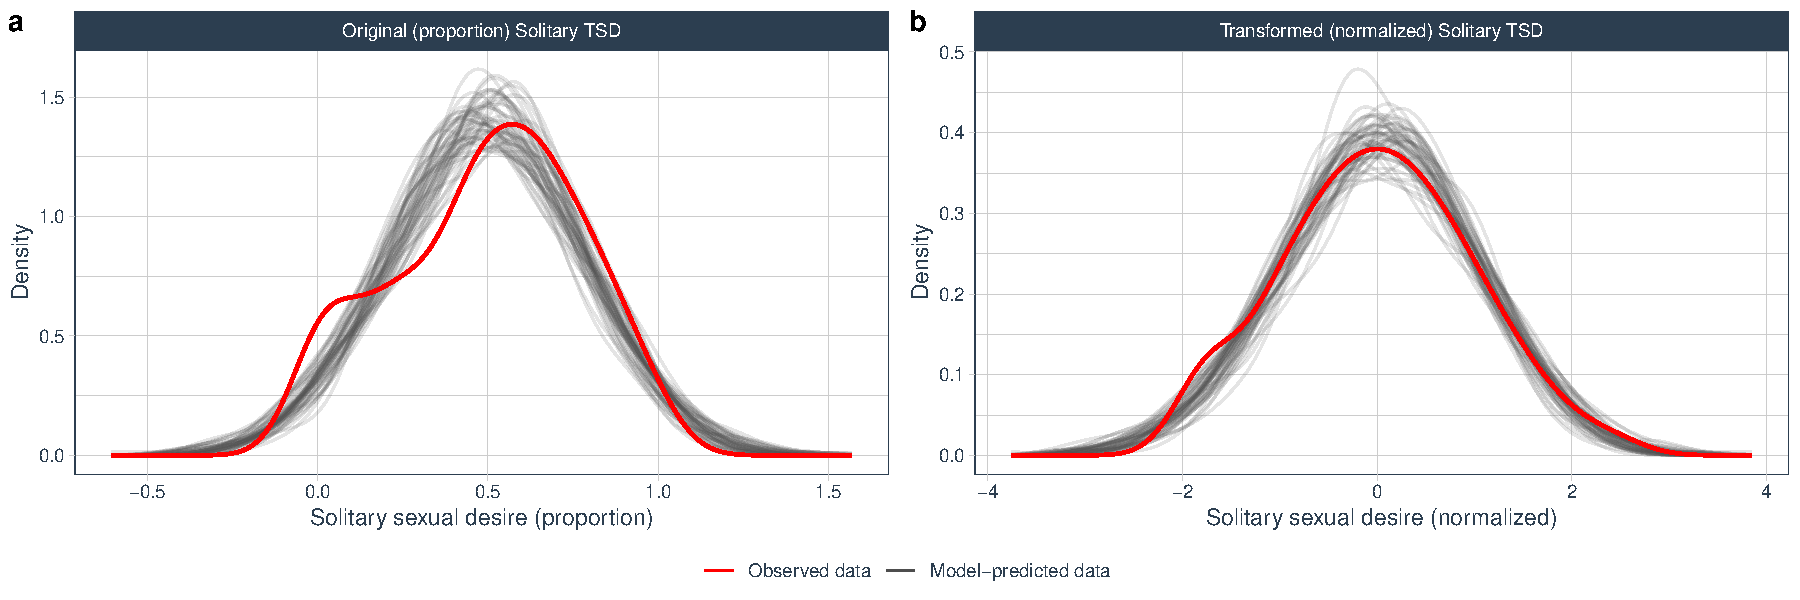
\includegraphics{Sexual_Desire_Arousal_V2_files/figure-latex/ppc-m1a-1.pdf}
\caption{\label{fig:ppc-m1a}Posterior predictive check. \textbf{(a)} Original (proportion) Solitary TSD; \textbf{(b)} Transformed (normalized) Solitary TSD. In both panels, red lines represent the observed data, and thin black lines represent 50 iterations of simulated data from each model.}
\end{figure}

\paragraph{\texorpdfstring{Table \ref{tab:tab-m1a}. Regression-type table for the interaction between \texttt{Relationship\ type}, and \texttt{Gender}}{Table \ref{tab:tab-m1a}. Regression-type table for the interaction between Relationship type, and Gender}}\label{table-reftabtab-m1a.-regression-type-table-for-the-interaction-between-relationship-type-and-gender}

This tables summarizes the results of the model.

\begin{Shaded}
\begin{Highlighting}[]
\FunctionTok{anova.sig}\NormalTok{(}\AttributeTok{model =}\NormalTok{ m1a\_norm, }\AttributeTok{custom\_caption =} \StringTok{"Effects of relationship type and gender on }
\StringTok{          solitary sexual desire"}\NormalTok{)}
\end{Highlighting}
\end{Shaded}

\begin{table}[H]
\centering
\caption{\label{tab:tab-m1a}Effects of relationship type and gender on 
          solitary sexual desire}
\centering
\resizebox{\ifdim\width>\linewidth\linewidth\else\width\fi}{!}{
\begin{threeparttable}
\begin{tabular}[t]{lcccl}
\toprule
Effect & $df$ & $F$ & $p$ & $\eta^2_G$\\
\midrule
Gender & 1, 319 & 19.01 & \textbf{< 0.0001} & 0.06\\
Relationship & 1, 319 & 8.36 & \textbf{0.004} & 0.03\\
Gender × Relationship & 1, 319 & 4.23 & \textbf{0.04} & 0.01\\
\bottomrule
\end{tabular}
\begin{tablenotes}[para]
\item \textit{Note: } 
\item Sexual desire was transformed using an ordered quantile 
                              normalization 
                              (\cite{petersonOrderedQuantileNormalization2020a}).
                              Results are type III ANOVA.
                              Gender = participants gender (women, men); 
                              Relationship = relationship type (stable, single).
                              As effect size, we used the generalized eta squared 
                              ($\eta^2_G$; see
                              \cite{bakemanRecommendedEffectSize2005}).
                              Significant effects are in bold.
\end{tablenotes}
\end{threeparttable}}
\end{table}

\paragraph{\texorpdfstring{\emph{Post-hoc} comparisons}{Post-hoc comparisons}}\label{post-hoc-comparisons}

Because the main effects of gender, relationship type, and their interaction are significant, we explored these effects using estimated marginal means.

\subparagraph{Table \ref{tab:tab-m1a-emm1}. Estimated marginal means and contrasts between participants' gender.}\label{table-reftabtab-m1a-emm1.-estimated-marginal-means-and-contrasts-between-participants-gender.}

Table of estimated marginal means and contrasts between genders. All estimated marginal means and contrasts were calculated using the \texttt{emmeans} function from the \texttt{emmeans} package \autocite{emmeanscit}.

\begin{Shaded}
\begin{Highlighting}[]
\NormalTok{emms.m1a1 }\OtherTok{\textless{}{-}} \FunctionTok{emmeans}\NormalTok{(m1a\_norm, }\SpecialCharTok{\textasciitilde{}}\NormalTok{ Gender)}

\NormalTok{emms.m1a1.tab }\OtherTok{\textless{}{-}} \FunctionTok{tibble}\NormalTok{(}\FunctionTok{data.frame}\NormalTok{(emms.m1a1))}

\NormalTok{t.m1a1 }\OtherTok{\textless{}{-}} \FunctionTok{contr.stars}\NormalTok{(emms.m1a1) }\SpecialCharTok{|\textgreater{}} 
  \FunctionTok{mutate}\NormalTok{(}\AttributeTok{p.value =} \FunctionTok{pval.lev}\NormalTok{(p.value))}

\FunctionTok{merge}\NormalTok{(emms.m1a1.tab, t.m1a1, }\AttributeTok{by =} \DecValTok{0}\NormalTok{, }\AttributeTok{all =} \ConstantTok{TRUE}\NormalTok{) }\SpecialCharTok{|\textgreater{}}
  \FunctionTok{select}\NormalTok{(}\SpecialCharTok{{-}}\FunctionTok{c}\NormalTok{(}\DecValTok{1}\NormalTok{,}\DecValTok{15}\NormalTok{)) }\SpecialCharTok{|\textgreater{}} 
  \FunctionTok{unite}\NormalTok{(Contrast, group1, group2, }\AttributeTok{sep =} \StringTok{" {-} "}\NormalTok{) }\SpecialCharTok{|\textgreater{}}
  \FunctionTok{mutate\_at}\NormalTok{(}\StringTok{"Contrast"}\NormalTok{, str\_replace\_all, }\StringTok{"NA {-} NA"}\NormalTok{, }\StringTok{" "}\NormalTok{) }\SpecialCharTok{|\textgreater{}} 
  \FunctionTok{kable}\NormalTok{(}\AttributeTok{digits =} \DecValTok{2}\NormalTok{,}
          \AttributeTok{booktabs =} \ConstantTok{TRUE}\NormalTok{,}
          \AttributeTok{align =} \FunctionTok{c}\NormalTok{(}\StringTok{"l"}\NormalTok{, }\FunctionTok{rep}\NormalTok{(}\StringTok{"c"}\NormalTok{, }\DecValTok{5}\NormalTok{), }\StringTok{"l"}\NormalTok{, }\FunctionTok{rep}\NormalTok{(}\StringTok{"c"}\NormalTok{, }\DecValTok{5}\NormalTok{)),}
          \AttributeTok{linesep =} \StringTok{""}\NormalTok{,}
          \AttributeTok{caption =} \StringTok{"Estimated marginal means and contrasts between participants\textquotesingle{} gender"}\NormalTok{,}
          \AttributeTok{col.names =} \FunctionTok{c}\NormalTok{(}\StringTok{"Gender"}\NormalTok{,}
                        \StringTok{"EMM"}\NormalTok{,}
                        \StringTok{"$SE$"}\NormalTok{,}
                        \StringTok{"$df$"}\NormalTok{,}
                        \StringTok{"$2.5}\SpecialCharTok{\textbackslash{}\textbackslash{}}\StringTok{\% CI$"}\NormalTok{,}
                        \StringTok{"$97.5}\SpecialCharTok{\textbackslash{}\textbackslash{}}\StringTok{\% CI$"}\NormalTok{,}
                        \StringTok{"Contrast"}\NormalTok{,}
                        \StringTok{"Difference"}\NormalTok{,}
                        \StringTok{"$SE$"}\NormalTok{,}
                        \StringTok{"$df$"}\NormalTok{,}
                        \StringTok{"$t$"}\NormalTok{,}
                        \StringTok{"$p$"}\NormalTok{),}
          \AttributeTok{escape =} \ConstantTok{FALSE}\NormalTok{) }\SpecialCharTok{|\textgreater{}}
  \FunctionTok{add\_header\_above}\NormalTok{(}\FunctionTok{c}\NormalTok{(}\StringTok{" "} \OtherTok{=} \DecValTok{6}\NormalTok{, }\StringTok{"Contrasts"} \OtherTok{=} \DecValTok{6}\NormalTok{)) }\SpecialCharTok{|\textgreater{}} 
  \FunctionTok{kable\_styling}\NormalTok{(}\AttributeTok{latex\_options =} \FunctionTok{c}\NormalTok{(}\StringTok{"HOLD\_position"}\NormalTok{, }\StringTok{"scale\_down"}\NormalTok{)) }\SpecialCharTok{|\textgreater{}}
  \FunctionTok{footnote}\NormalTok{(}\AttributeTok{general =} \StringTok{"Significant effects are in bold."}\NormalTok{,}
           \AttributeTok{threeparttable =} \ConstantTok{TRUE}\NormalTok{,}
           \AttributeTok{footnote\_as\_chunk =} \ConstantTok{TRUE}\NormalTok{,}
           \AttributeTok{escape =} \ConstantTok{FALSE}\NormalTok{)}
\end{Highlighting}
\end{Shaded}

\begin{table}[H]
\centering
\caption{\label{tab:tab-m1a-emm1}Estimated marginal means and contrasts between participants' gender}
\centering
\resizebox{\ifdim\width>\linewidth\linewidth\else\width\fi}{!}{
\begin{threeparttable}
\begin{tabular}[t]{lccccclccccc}
\toprule
\multicolumn{6}{c}{ } & \multicolumn{6}{c}{Contrasts} \\
\cmidrule(l{3pt}r{3pt}){7-12}
Gender & EMM & $SE$ & $df$ & $2.5\% CI$ & $97.5\% CI$ & Contrast & Difference & $SE$ & $df$ & $t$ & $p$\\
\midrule
Women & -0.17 & 0.07 & 319 & -0.30 & -0.03 & Women - Men & -0.46 & 0.1 & 319 & -4.36 & \textbf{< 0.0001}\\
Men & 0.29 & 0.08 & 319 & 0.13 & 0.44 &  &  &  &  &  & \\
\bottomrule
\end{tabular}
\begin{tablenotes}[para]
\item \textit{Note: } 
\item Significant effects are in bold.
\end{tablenotes}
\end{threeparttable}}
\end{table}

\subparagraph{Table \ref{tab:tab-m1a-emm2}. Estimated marginal means and contrasts between relationship status.}\label{table-reftabtab-m1a-emm2.-estimated-marginal-means-and-contrasts-between-relationship-status.}

Table of estimated marginal means and contrasts between relationship status. All estimated marginal means and contrasts were calculated using the \texttt{emmeans} function from the \texttt{emmeans} package \autocite{emmeanscit}.

\begin{Shaded}
\begin{Highlighting}[]
\NormalTok{emms.m1a2 }\OtherTok{\textless{}{-}} \FunctionTok{emmeans}\NormalTok{(m1a\_norm, }\SpecialCharTok{\textasciitilde{}}\NormalTok{ Relationship)}

\NormalTok{emms.m1a2.tab }\OtherTok{\textless{}{-}} \FunctionTok{tibble}\NormalTok{(}\FunctionTok{data.frame}\NormalTok{(emms.m1a2))}

\NormalTok{t.m1a2 }\OtherTok{\textless{}{-}} \FunctionTok{contr.stars}\NormalTok{(emms.m1a2) }\SpecialCharTok{|\textgreater{}} 
  \FunctionTok{mutate}\NormalTok{(}\AttributeTok{p.value =} \FunctionTok{pval.lev}\NormalTok{(p.value))}

\FunctionTok{merge}\NormalTok{(emms.m1a2.tab, t.m1a2, }\AttributeTok{by =} \DecValTok{0}\NormalTok{, }\AttributeTok{all =} \ConstantTok{TRUE}\NormalTok{) }\SpecialCharTok{|\textgreater{}}
  \FunctionTok{select}\NormalTok{(}\SpecialCharTok{{-}}\FunctionTok{c}\NormalTok{(}\DecValTok{1}\NormalTok{,}\DecValTok{15}\NormalTok{)) }\SpecialCharTok{|\textgreater{}} 
  \FunctionTok{unite}\NormalTok{(Contrast, group1, group2, }\AttributeTok{sep =} \StringTok{" {-} "}\NormalTok{) }\SpecialCharTok{|\textgreater{}}
  \FunctionTok{mutate\_at}\NormalTok{(}\StringTok{"Contrast"}\NormalTok{, str\_replace\_all, }\StringTok{"NA {-} NA"}\NormalTok{, }\StringTok{" "}\NormalTok{) }\SpecialCharTok{|\textgreater{}} 
  \FunctionTok{kable}\NormalTok{(}\AttributeTok{digits =} \DecValTok{2}\NormalTok{,}
          \AttributeTok{booktabs =} \ConstantTok{TRUE}\NormalTok{,}
          \AttributeTok{align =} \FunctionTok{c}\NormalTok{(}\StringTok{"l"}\NormalTok{, }\FunctionTok{rep}\NormalTok{(}\StringTok{"c"}\NormalTok{, }\DecValTok{5}\NormalTok{), }\StringTok{"l"}\NormalTok{, }\FunctionTok{rep}\NormalTok{(}\StringTok{"c"}\NormalTok{, }\DecValTok{5}\NormalTok{)),}
          \AttributeTok{linesep =} \StringTok{""}\NormalTok{,}
          \AttributeTok{caption =} \StringTok{"Estimated marginal means and contrasts between relationship status"}\NormalTok{,}
          \AttributeTok{col.names =} \FunctionTok{c}\NormalTok{(}\StringTok{"Relationship type"}\NormalTok{,}
                        \StringTok{"EMM"}\NormalTok{,}
                        \StringTok{"$SE$"}\NormalTok{,}
                        \StringTok{"$df$"}\NormalTok{,}
                        \StringTok{"$2.5}\SpecialCharTok{\textbackslash{}\textbackslash{}}\StringTok{\% CI$"}\NormalTok{,}
                        \StringTok{"$97.5}\SpecialCharTok{\textbackslash{}\textbackslash{}}\StringTok{\% CI$"}\NormalTok{,}
                        \StringTok{"Contrast"}\NormalTok{,}
                        \StringTok{"Difference"}\NormalTok{,}
                        \StringTok{"$SE$"}\NormalTok{,}
                        \StringTok{"$df$"}\NormalTok{,}
                        \StringTok{"$t$"}\NormalTok{,}
                        \StringTok{"$p$"}\NormalTok{),}
          \AttributeTok{escape =} \ConstantTok{FALSE}\NormalTok{) }\SpecialCharTok{|\textgreater{}}
  \FunctionTok{add\_header\_above}\NormalTok{(}\FunctionTok{c}\NormalTok{(}\StringTok{" "} \OtherTok{=} \DecValTok{6}\NormalTok{, }\StringTok{"Contrasts"} \OtherTok{=} \DecValTok{6}\NormalTok{)) }\SpecialCharTok{|\textgreater{}} 
  \FunctionTok{kable\_styling}\NormalTok{(}\AttributeTok{latex\_options =} \FunctionTok{c}\NormalTok{(}\StringTok{"HOLD\_position"}\NormalTok{, }\StringTok{"scale\_down"}\NormalTok{)) }\SpecialCharTok{|\textgreater{}}
  \FunctionTok{footnote}\NormalTok{(}\AttributeTok{general =} \StringTok{"Significant effects are in bold."}\NormalTok{,}
           \AttributeTok{threeparttable =} \ConstantTok{TRUE}\NormalTok{,}
           \AttributeTok{footnote\_as\_chunk =} \ConstantTok{TRUE}\NormalTok{,}
           \AttributeTok{escape =} \ConstantTok{FALSE}\NormalTok{)}
\end{Highlighting}
\end{Shaded}

\begin{table}[H]
\centering
\caption{\label{tab:tab-m1a-emm2}Estimated marginal means and contrasts between relationship status}
\centering
\resizebox{\ifdim\width>\linewidth\linewidth\else\width\fi}{!}{
\begin{threeparttable}
\begin{tabular}[t]{lccccclccccc}
\toprule
\multicolumn{6}{c}{ } & \multicolumn{6}{c}{Contrasts} \\
\cmidrule(l{3pt}r{3pt}){7-12}
Relationship type & EMM & $SE$ & $df$ & $2.5\% CI$ & $97.5\% CI$ & Contrast & Difference & $SE$ & $df$ & $t$ & $p$\\
\midrule
Stable & -0.09 & 0.07 & 319 & -0.23 & 0.05 & Stable - Single & -0.3 & 0.1 & 319 & -2.89 & \textbf{0.0041}\\
Single & 0.21 & 0.08 & 319 & 0.06 & 0.36 &  &  &  &  &  & \\
\bottomrule
\end{tabular}
\begin{tablenotes}[para]
\item \textit{Note: } 
\item Significant effects are in bold.
\end{tablenotes}
\end{threeparttable}}
\end{table}

\subparagraph{Table \ref{tab:tab-m1a-emm3}. Estimated marginal means and contrasts between gender by relationship status.}\label{table-reftabtab-m1a-emm3.-estimated-marginal-means-and-contrasts-between-gender-by-relationship-status.}

Table of estimated marginal means and contrasts between gender by relationship status. All estimated marginal means and contrasts were calculated using the \texttt{emmeans} function from the \texttt{emmeans} package \autocite{emmeanscit}.

\begin{Shaded}
\begin{Highlighting}[]
\NormalTok{emms.m1a3 }\OtherTok{\textless{}{-}} \FunctionTok{emmeans}\NormalTok{(m1a\_norm, }\SpecialCharTok{\textasciitilde{}}\NormalTok{ Gender }\SpecialCharTok{|}\NormalTok{ Relationship)}

\NormalTok{emms.m1a3.tab }\OtherTok{\textless{}{-}} \FunctionTok{tibble}\NormalTok{(}\FunctionTok{data.frame}\NormalTok{(emms.m1a3))}

\NormalTok{t.m1a3 }\OtherTok{\textless{}{-}} \FunctionTok{contr.stars}\NormalTok{(emms.m1a3) }\SpecialCharTok{|\textgreater{}} 
  \FunctionTok{mutate}\NormalTok{(}\AttributeTok{p.value =} \FunctionTok{pval.lev}\NormalTok{(p.value))}

\NormalTok{t.m1a3.f }\OtherTok{\textless{}{-}}\NormalTok{ t.m1a3 }\SpecialCharTok{|\textgreater{}} 
  \FunctionTok{insertRows}\NormalTok{(}\DecValTok{2}\NormalTok{, }\AttributeTok{new =} \ConstantTok{NA}\NormalTok{) }\SpecialCharTok{|\textgreater{}}
\FunctionTok{insertRows}\NormalTok{(}\DecValTok{4}\NormalTok{, }\AttributeTok{new =} \ConstantTok{NA}\NormalTok{)}

\FunctionTok{merge}\NormalTok{(emms.m1a3.tab, t.m1a3.f, }\AttributeTok{by =} \DecValTok{0}\NormalTok{, }\AttributeTok{all =} \ConstantTok{TRUE}\NormalTok{) }\SpecialCharTok{|\textgreater{}}
  \FunctionTok{select}\NormalTok{(}\SpecialCharTok{{-}}\FunctionTok{c}\NormalTok{(}\DecValTok{1}\NormalTok{,}\DecValTok{3}\NormalTok{,}\DecValTok{11}\NormalTok{,}\DecValTok{17}\NormalTok{)) }\SpecialCharTok{|\textgreater{}} 
  \FunctionTok{drop\_na}\NormalTok{(Gender) }\SpecialCharTok{|\textgreater{}} 
  \FunctionTok{unite}\NormalTok{(Contrast, group1, group2, }\AttributeTok{sep =} \StringTok{" {-} "}\NormalTok{) }\SpecialCharTok{|\textgreater{}}
  \FunctionTok{mutate\_at}\NormalTok{(}\StringTok{"Contrast"}\NormalTok{, str\_replace\_all, }\StringTok{"NA {-} NA"}\NormalTok{, }\StringTok{""}\NormalTok{) }\SpecialCharTok{|\textgreater{}} 
  \FunctionTok{kable}\NormalTok{(}\AttributeTok{digits =} \DecValTok{2}\NormalTok{,}
          \AttributeTok{booktabs =} \ConstantTok{TRUE}\NormalTok{,}
          \AttributeTok{align =} \FunctionTok{c}\NormalTok{(}\StringTok{"l"}\NormalTok{, }\StringTok{"l"}\NormalTok{, }\FunctionTok{rep}\NormalTok{(}\StringTok{"c"}\NormalTok{, }\DecValTok{5}\NormalTok{), }\StringTok{"l"}\NormalTok{, }\FunctionTok{rep}\NormalTok{(}\StringTok{"c"}\NormalTok{, }\DecValTok{5}\NormalTok{)),}
          \AttributeTok{linesep =} \StringTok{""}\NormalTok{,}
          \AttributeTok{caption =} \StringTok{"Estimated marginal means and contrasts between gender by }
\StringTok{                    relationship status"}\NormalTok{,}
          \AttributeTok{col.names =} \FunctionTok{c}\NormalTok{(}\StringTok{"Gender"}\NormalTok{,}
                        \CommentTok{\#"Relationship",}
                        \StringTok{"EMM"}\NormalTok{,}
                        \StringTok{"$SE$"}\NormalTok{,}
                        \StringTok{"$df$"}\NormalTok{,}
                        \StringTok{"$2.5}\SpecialCharTok{\textbackslash{}\textbackslash{}}\StringTok{\% CI$"}\NormalTok{,}
                        \StringTok{"$97.5}\SpecialCharTok{\textbackslash{}\textbackslash{}}\StringTok{\% CI$"}\NormalTok{,}
                        \StringTok{"Contrast"}\NormalTok{,}
                        \StringTok{"Difference"}\NormalTok{,}
                        \StringTok{"$SE$"}\NormalTok{,}
                        \StringTok{"$df$"}\NormalTok{,}
                        \StringTok{"$t$"}\NormalTok{,}
                        \StringTok{"$p$"}\NormalTok{),}
          \AttributeTok{escape =} \ConstantTok{FALSE}\NormalTok{) }\SpecialCharTok{|\textgreater{}}
  \FunctionTok{pack\_rows}\NormalTok{(}\AttributeTok{group\_label =} \StringTok{"Relationship status: Stable"}\NormalTok{,}
            \AttributeTok{start\_row =} \DecValTok{1}\NormalTok{,}
            \AttributeTok{end\_row =} \DecValTok{2}\NormalTok{,}
            \AttributeTok{hline\_before =} \ConstantTok{FALSE}\NormalTok{,}
            \AttributeTok{bold =} \ConstantTok{TRUE}\NormalTok{) }\SpecialCharTok{|\textgreater{}}
  \FunctionTok{pack\_rows}\NormalTok{(}\AttributeTok{group\_label =} \StringTok{"Relationship status: Single"}\NormalTok{,}
            \AttributeTok{start\_row =} \DecValTok{3}\NormalTok{,}
            \AttributeTok{end\_row =} \DecValTok{4}\NormalTok{,}
            \AttributeTok{hline\_before =} \ConstantTok{TRUE}\NormalTok{,}
            \AttributeTok{bold =} \ConstantTok{TRUE}\NormalTok{) }\SpecialCharTok{|\textgreater{}}
  \FunctionTok{add\_header\_above}\NormalTok{(}\FunctionTok{c}\NormalTok{(}\StringTok{" "} \OtherTok{=} \DecValTok{6}\NormalTok{, }\StringTok{"Contrasts"} \OtherTok{=} \DecValTok{6}\NormalTok{)) }\SpecialCharTok{|\textgreater{}} 
  \FunctionTok{kable\_styling}\NormalTok{(}\AttributeTok{latex\_options =} \FunctionTok{c}\NormalTok{(}\StringTok{"HOLD\_position"}\NormalTok{, }\StringTok{"scale\_down"}\NormalTok{)) }\SpecialCharTok{|\textgreater{}}
  \FunctionTok{footnote}\NormalTok{(}\AttributeTok{general =} \StringTok{"Significant effects are in bold."}\NormalTok{,}
           \AttributeTok{threeparttable =} \ConstantTok{TRUE}\NormalTok{,}
           \AttributeTok{footnote\_as\_chunk =} \ConstantTok{TRUE}\NormalTok{,}
           \AttributeTok{escape =} \ConstantTok{FALSE}\NormalTok{)}
\end{Highlighting}
\end{Shaded}

\begin{table}[H]
\centering
\caption{\label{tab:tab-m1a-emm3}Estimated marginal means and contrasts between gender by 
                    relationship status}
\centering
\resizebox{\ifdim\width>\linewidth\linewidth\else\width\fi}{!}{
\begin{threeparttable}
\begin{tabular}[t]{llccccclcccc}
\toprule
\multicolumn{6}{c}{ } & \multicolumn{6}{c}{Contrasts} \\
\cmidrule(l{3pt}r{3pt}){7-12}
Gender & EMM & $SE$ & $df$ & $2.5\% CI$ & $97.5\% CI$ & Contrast & Difference & $SE$ & $df$ & $t$ & $p$\\
\midrule
\addlinespace[0.3em]
\multicolumn{12}{l}{\textbf{Relationship status: Stable}}\\
\hspace{1em}Women & -0.43 & 0.09 & 319 & -0.61 & -0.25 & Women - Men & -0.67 & 0.14 & 319 & -4.74 & \textbf{< 0.0001}\\
\hspace{1em}Men & 0.24 & 0.11 & 319 & 0.03 & 0.46 &  &  &  &  &  & \\
\addlinespace[0.3em]
\hline
\multicolumn{12}{l}{\textbf{Relationship status: Single}}\\
\hspace{1em}Women & 0.09 & 0.10 & 319 & -0.11 & 0.30 & Women - Men & -0.24 & 0.15 & 319 & -1.57 & 0.12\\
\hspace{1em}Men & 0.33 & 0.11 & 319 & 0.11 & 0.55 &  &  &  &  &  & \\
\bottomrule
\end{tabular}
\begin{tablenotes}[para]
\item \textit{Note: } 
\item Significant effects are in bold.
\end{tablenotes}
\end{threeparttable}}
\end{table}

\paragraph{Figure \ref{fig:fig-h1a}. Differences among the three dimensions of sexual desire}\label{figure-reffigfig-h1a.-differences-among-the-three-dimensions-of-sexual-desire}

This figure summarizes the results of hypothesis 1a.

\begin{Shaded}
\begin{Highlighting}[]
\CommentTok{\# Gender main effect}
\NormalTok{h1a1 }\OtherTok{\textless{}{-}} \FunctionTok{ggplot}\NormalTok{(dat\_m1, }\FunctionTok{aes}\NormalTok{(}\AttributeTok{x =}\NormalTok{ Gender, }\AttributeTok{y =} \StringTok{\textasciigrave{}}\AttributeTok{Solitary sexual desire (normalized)}\StringTok{\textasciigrave{}}\NormalTok{, }
                          \AttributeTok{color =}\NormalTok{ Gender)) }\SpecialCharTok{+}
  \FunctionTok{geom\_violin}\NormalTok{(}\AttributeTok{trim =} \ConstantTok{FALSE}\NormalTok{) }\SpecialCharTok{+}
  \FunctionTok{geom\_jitter}\NormalTok{(}\AttributeTok{alpha =} \FloatTok{0.3}\NormalTok{, }\AttributeTok{width =} \FloatTok{0.1}\NormalTok{) }\SpecialCharTok{+}
  \FunctionTok{scale\_color\_manual}\NormalTok{(}\AttributeTok{values =}\NormalTok{ color.Gender) }\SpecialCharTok{+}
  \FunctionTok{scale\_fill\_manual}\NormalTok{(}\AttributeTok{values =}\NormalTok{ color.Gender) }\SpecialCharTok{+}
  \FunctionTok{geom\_errorbar}\NormalTok{(}\AttributeTok{data =}\NormalTok{ emms.m1a1.tab }\SpecialCharTok{|\textgreater{}} 
                  \FunctionTok{rename}\NormalTok{(}\StringTok{\textquotesingle{}Solitary sexual desire (normalized)\textquotesingle{}} \OtherTok{=}\NormalTok{ emmean),}
                \AttributeTok{mapping =} \FunctionTok{aes}\NormalTok{(}\AttributeTok{ymin =}\NormalTok{ lower.CL, }\AttributeTok{ymax =}\NormalTok{ upper.CL), }
                \AttributeTok{colour =} \StringTok{"black"}\NormalTok{, }\AttributeTok{width =} \FloatTok{0.1}\NormalTok{) }\SpecialCharTok{+}
  \FunctionTok{geom\_point}\NormalTok{(}\AttributeTok{data =}\NormalTok{ emms.m1a1.tab }\SpecialCharTok{|\textgreater{}} 
                  \FunctionTok{rename}\NormalTok{(}\StringTok{\textquotesingle{}Solitary sexual desire (normalized)\textquotesingle{}} \OtherTok{=}\NormalTok{ emmean), }
             \AttributeTok{position =} \FunctionTok{position\_dodge}\NormalTok{(}\FloatTok{0.1}\NormalTok{), }
             \AttributeTok{shape =} \DecValTok{21}\NormalTok{, }\AttributeTok{size =} \DecValTok{3}\NormalTok{,}
             \AttributeTok{color =} \StringTok{"black"}\NormalTok{, }\AttributeTok{fill =} \StringTok{"white"}\NormalTok{) }\SpecialCharTok{+}
  \FunctionTok{stat\_pvalue\_manual}\NormalTok{(t.m1a1, }
                     \AttributeTok{label =} \StringTok{"p.signif"}\NormalTok{, }
                     \AttributeTok{y.position =} \FloatTok{3.5}\NormalTok{, }
                     \AttributeTok{tip.length =} \DecValTok{0}\NormalTok{) }\SpecialCharTok{+}
  \FunctionTok{guides}\NormalTok{(}\AttributeTok{color =} \StringTok{"none"}\NormalTok{) }\SpecialCharTok{+}
  \FunctionTok{theme\_tq}\NormalTok{()}

\CommentTok{\# Relationship main effect}
\NormalTok{h1a2 }\OtherTok{\textless{}{-}} \FunctionTok{ggplot}\NormalTok{(dat\_m1, }\FunctionTok{aes}\NormalTok{(}\AttributeTok{x =}\NormalTok{ Relationship, }\AttributeTok{y =} \StringTok{\textasciigrave{}}\AttributeTok{Solitary sexual desire (normalized)}\StringTok{\textasciigrave{}}\NormalTok{, }
                          \AttributeTok{color =}\NormalTok{ Relationship)) }\SpecialCharTok{+}
  \FunctionTok{geom\_violin}\NormalTok{(}\AttributeTok{trim =} \ConstantTok{FALSE}\NormalTok{) }\SpecialCharTok{+}
  \FunctionTok{geom\_jitter}\NormalTok{(}\AttributeTok{alpha =} \FloatTok{0.3}\NormalTok{, }\AttributeTok{width =} \FloatTok{0.1}\NormalTok{) }\SpecialCharTok{+}
  \FunctionTok{scale\_color\_manual}\NormalTok{(}\AttributeTok{values =}\NormalTok{ color.Relationship) }\SpecialCharTok{+}
  \FunctionTok{scale\_fill\_manual}\NormalTok{(}\AttributeTok{values =}\NormalTok{ color.Relationship) }\SpecialCharTok{+}
  \FunctionTok{geom\_errorbar}\NormalTok{(}\AttributeTok{data =}\NormalTok{ emms.m1a2.tab }\SpecialCharTok{|\textgreater{}} 
                  \FunctionTok{rename}\NormalTok{(}\StringTok{\textquotesingle{}Solitary sexual desire (normalized)\textquotesingle{}} \OtherTok{=}\NormalTok{ emmean),}
                \AttributeTok{mapping =} \FunctionTok{aes}\NormalTok{(}\AttributeTok{ymin =}\NormalTok{ lower.CL, }\AttributeTok{ymax =}\NormalTok{ upper.CL), }
                \AttributeTok{colour =} \StringTok{"black"}\NormalTok{, }\AttributeTok{width =} \FloatTok{0.1}\NormalTok{) }\SpecialCharTok{+}
  \FunctionTok{geom\_point}\NormalTok{(}\AttributeTok{data =}\NormalTok{ emms.m1a2.tab }\SpecialCharTok{|\textgreater{}} 
                  \FunctionTok{rename}\NormalTok{(}\StringTok{\textquotesingle{}Solitary sexual desire (normalized)\textquotesingle{}} \OtherTok{=}\NormalTok{ emmean), }
             \AttributeTok{position =} \FunctionTok{position\_dodge}\NormalTok{(}\FloatTok{0.1}\NormalTok{), }
             \AttributeTok{shape =} \DecValTok{21}\NormalTok{, }\AttributeTok{size =} \DecValTok{3}\NormalTok{,}
             \AttributeTok{color =} \StringTok{"black"}\NormalTok{, }\AttributeTok{fill =} \StringTok{"white"}\NormalTok{) }\SpecialCharTok{+}
  \FunctionTok{stat\_pvalue\_manual}\NormalTok{(t.m1a2, }
                     \AttributeTok{label =} \StringTok{"p.signif"}\NormalTok{, }
                     \AttributeTok{y.position =} \FloatTok{3.5}\NormalTok{, }
                     \AttributeTok{tip.length =} \DecValTok{0}\NormalTok{) }\SpecialCharTok{+}
  \FunctionTok{guides}\NormalTok{(}\AttributeTok{color =} \StringTok{"none"}\NormalTok{) }\SpecialCharTok{+}
  \FunctionTok{theme\_tq}\NormalTok{()}

\CommentTok{\# Relationship × Gender interaction}
\NormalTok{h1a3 }\OtherTok{\textless{}{-}} \FunctionTok{ggplot}\NormalTok{(dat\_m1, }\FunctionTok{aes}\NormalTok{(}\AttributeTok{x =}\NormalTok{ Gender, }\AttributeTok{y =} \StringTok{\textasciigrave{}}\AttributeTok{Solitary sexual desire (normalized)}\StringTok{\textasciigrave{}}\NormalTok{, }
                           \AttributeTok{color =}\NormalTok{ Gender)) }\SpecialCharTok{+}
  \FunctionTok{geom\_violin}\NormalTok{(}\AttributeTok{trim =} \ConstantTok{FALSE}\NormalTok{) }\SpecialCharTok{+}
  \FunctionTok{geom\_jitter}\NormalTok{(}\AttributeTok{alpha =} \FloatTok{0.3}\NormalTok{, }\AttributeTok{width =} \FloatTok{0.1}\NormalTok{) }\SpecialCharTok{+}
  \FunctionTok{scale\_color\_manual}\NormalTok{(}\AttributeTok{values =}\NormalTok{ color.Gender) }\SpecialCharTok{+}
  \FunctionTok{scale\_fill\_manual}\NormalTok{(}\AttributeTok{values =}\NormalTok{ color.Gender) }\SpecialCharTok{+}
  \FunctionTok{facet\_wrap}\NormalTok{(}\SpecialCharTok{\textasciitilde{}}\NormalTok{Relationship) }\SpecialCharTok{+}
  \FunctionTok{geom\_errorbar}\NormalTok{(}\AttributeTok{data =}\NormalTok{ emms.m1a3.tab }\SpecialCharTok{|\textgreater{}} 
                  \FunctionTok{rename}\NormalTok{(}\StringTok{\textquotesingle{}Solitary sexual desire (normalized)\textquotesingle{}} \OtherTok{=}\NormalTok{ emmean), }
                \AttributeTok{mapping =} \FunctionTok{aes}\NormalTok{(}\AttributeTok{ymin =}\NormalTok{ lower.CL, }\AttributeTok{ymax =}\NormalTok{ upper.CL), }
                \AttributeTok{colour =} \StringTok{"black"}\NormalTok{, }\AttributeTok{width =} \FloatTok{0.1}\NormalTok{) }\SpecialCharTok{+}
  \FunctionTok{geom\_point}\NormalTok{(}\AttributeTok{data =}\NormalTok{ emms.m1a3.tab}\SpecialCharTok{|\textgreater{}} 
                  \FunctionTok{rename}\NormalTok{(}\StringTok{\textquotesingle{}Solitary sexual desire (normalized)\textquotesingle{}} \OtherTok{=}\NormalTok{ emmean), }
             \AttributeTok{position =} \FunctionTok{position\_dodge}\NormalTok{(}\FloatTok{0.1}\NormalTok{), }
             \AttributeTok{shape =} \DecValTok{21}\NormalTok{, }\AttributeTok{size =} \DecValTok{3}\NormalTok{,}
             \AttributeTok{color =} \StringTok{"black"}\NormalTok{, }\AttributeTok{fill =} \StringTok{"white"}\NormalTok{) }\SpecialCharTok{+}
  \FunctionTok{stat\_pvalue\_manual}\NormalTok{(t.m1a3, }
                     \AttributeTok{label =} \StringTok{"p.signif"}\NormalTok{, }
                     \AttributeTok{y.position =} \FloatTok{3.5}\NormalTok{, }
                     \AttributeTok{tip.length =} \DecValTok{0}\NormalTok{) }\SpecialCharTok{+}
  \FunctionTok{guides}\NormalTok{(}\AttributeTok{color =} \StringTok{"none"}\NormalTok{) }\SpecialCharTok{+}
  \FunctionTok{theme\_tq}\NormalTok{()}

\CommentTok{\# Full figure for hypothesis 1 (a, b and c)}
\NormalTok{p1a }\OtherTok{\textless{}{-}} \FunctionTok{ggarrange}\NormalTok{(h1a1, h1a2, h1a3,}
                 \AttributeTok{ncol =} \DecValTok{3}\NormalTok{,}
                 \AttributeTok{labels =} \StringTok{"auto"}\NormalTok{,}
                 \AttributeTok{widths =} \FunctionTok{c}\NormalTok{(}\DecValTok{1}\NormalTok{,}\DecValTok{1}\NormalTok{,}\FloatTok{1.5}\NormalTok{))}
\NormalTok{p1a}
\end{Highlighting}
\end{Shaded}

\begin{figure}
\centering
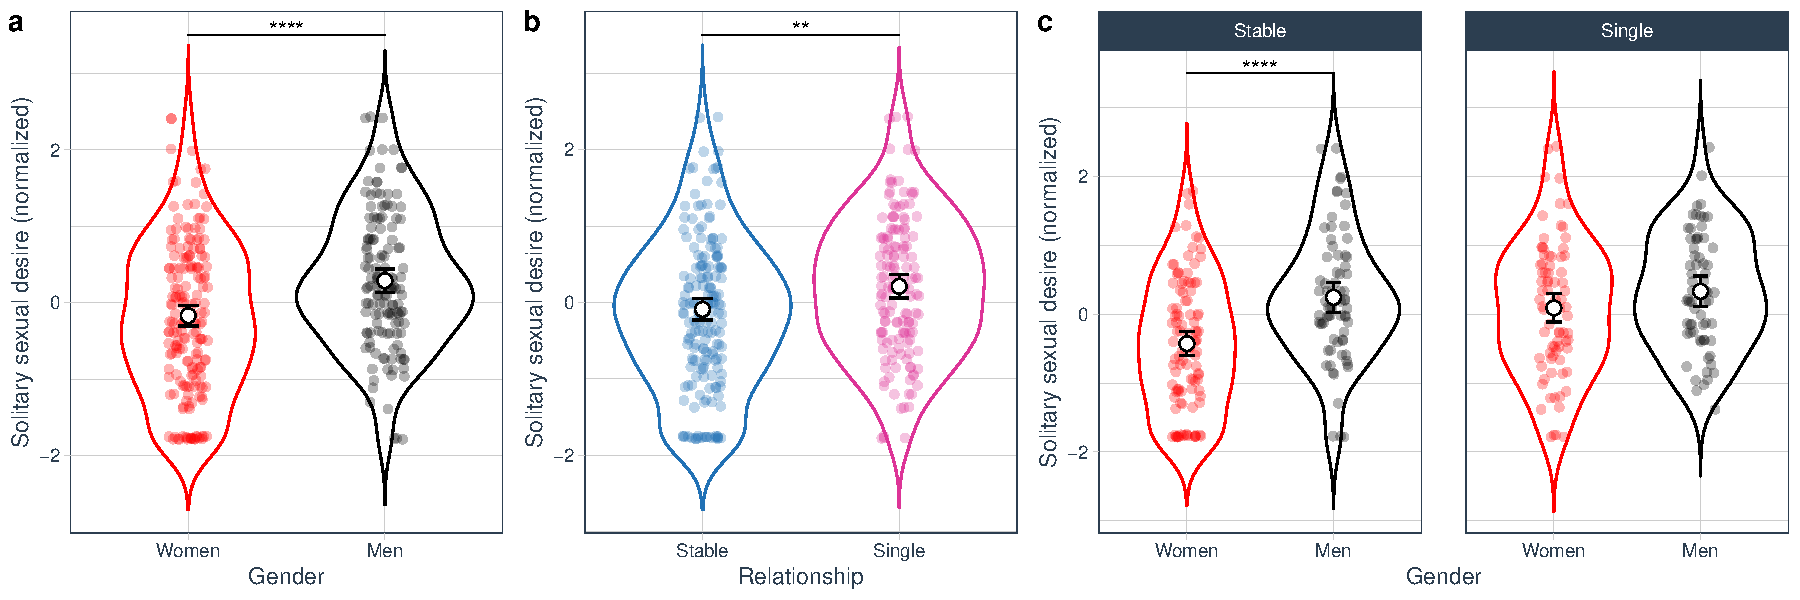
\includegraphics{Sexual_Desire_Arousal_V2_files/figure-latex/fig-h1a-1.pdf}
\caption{\label{fig:fig-h1a}Effects of gender and relationship type on solitary sexual desire. Solitary sexual desire was transformed using ordered quantile normalization \autocite{petersonOrderedQuantileNormalization2020a}. \textbf{(a)} Simple comparison between sexual desire by gender (for detailed results, see Table \ref{tab:tab-m1a-emm1}); \textbf{(b)} Simple comparison between relationship status levels (for detailed results, see Table \ref{tab:tab-m1a-emm2}); \textbf{(c)} Interaction between relationship type and relationship status (see Table \ref{tab:tab-m1a}; for detailed results, see Table \ref{tab:tab-m1a-emm3}). White dots and black bars represent estimated marginal means and 95\% CI. In all cases, significant effects are represented with lines and stars: *\emph{p} \textless{} 0.05, **\emph{p} \textless{} 0.01, ***\emph{p} \textless{} 0.001, ****\emph{p} \textless{} 0.0001.}
\end{figure}

\subsubsection{Hypothesis 1b: Solitary TSD}\label{hypothesis1b}

\paragraph{Model the effects of relationship type and gender on Solitary TSD}\label{model-the-effects-of-relationship-type-and-gender-on-solitary-tsd-1}

We fitted models with both the original (proportion; \texttt{m1b\_prop}) and transformed (normalized; \texttt{m1b\_norm}) TSD scores, and performed posterior predictive checks (PPCs). As shown elsewhere \autocite[e.g.,][]{gabryVisualizationBayesianWorkflow2019}, if simulated data from one model are more similar to the observed outcome, that model is likely to be preferred.

\begin{Shaded}
\begin{Highlighting}[]
\FunctionTok{options}\NormalTok{(}\AttributeTok{contrasts =} \FunctionTok{c}\NormalTok{(}\StringTok{"contr.sum"}\NormalTok{,}\StringTok{"contr.poly"}\NormalTok{))}
\NormalTok{m1b\_prop }\OtherTok{\textless{}{-}} \FunctionTok{lm}\NormalTok{(}\StringTok{\textasciigrave{}}\AttributeTok{Dyadic sexual desire: Attractive person (proportion)}\StringTok{\textasciigrave{}} \SpecialCharTok{\textasciitilde{}}\NormalTok{ Gender }\SpecialCharTok{*}\NormalTok{ Relationship,}
            \AttributeTok{data =}\NormalTok{ dat\_m1)}

\NormalTok{m1b\_norm }\OtherTok{\textless{}{-}} \FunctionTok{lm}\NormalTok{(}\StringTok{\textasciigrave{}}\AttributeTok{Dyadic sexual desire: Attractive person (normalized)}\StringTok{\textasciigrave{}} \SpecialCharTok{\textasciitilde{}}\NormalTok{ Gender }\SpecialCharTok{*}\NormalTok{ Relationship,}
           \AttributeTok{data =}\NormalTok{ dat\_m1)}
\end{Highlighting}
\end{Shaded}

\subparagraph{Figure \ref{fig:ppc-m1b}: Posterior predictive checks (PPCs) for Hypothesis 1b.}\label{figure-reffigppc-m1b-posterior-predictive-checks-ppcs-for-hypothesis-1b.}

PPCs were performed using the \texttt{check\_model} function from the \texttt{performance} package \autocite{ludecke2021}, and reported in Fig. \ref{fig:ppc-m1b}. Simulated data from the normalized Solitary TSD model (Fig. \ref{fig:ppc-m1b}b) are more similar to the observed outcome, so this model is preferred.

\begin{Shaded}
\begin{Highlighting}[]
\NormalTok{ppc\_m1b }\OtherTok{\textless{}{-}} \FunctionTok{ggarrange}\NormalTok{(}\FunctionTok{plot}\NormalTok{(}\FunctionTok{check\_model}\NormalTok{(m1b\_prop, }
                                      \AttributeTok{panel =} \ConstantTok{FALSE}\NormalTok{,}
                                      \AttributeTok{check =} \StringTok{"pp\_check"}\NormalTok{)}\SpecialCharTok{$}\NormalTok{PP\_CHECK,}
                          \AttributeTok{colors =} \FunctionTok{c}\NormalTok{(}\StringTok{"red"}\NormalTok{, }\StringTok{"grey30"}\NormalTok{)) }\SpecialCharTok{+}
                       \FunctionTok{labs}\NormalTok{(}\AttributeTok{title =} \ConstantTok{NULL}\NormalTok{, }\AttributeTok{subtitle =} \ConstantTok{NULL}\NormalTok{) }\SpecialCharTok{+}
                       \FunctionTok{theme\_tq}\NormalTok{() }\SpecialCharTok{+}
                       \FunctionTok{facet\_wrap}\NormalTok{(}\SpecialCharTok{\textasciitilde{}} \DecValTok{1}\NormalTok{, }\AttributeTok{labeller =} \FunctionTok{as\_labeller}\NormalTok{(}\FunctionTok{c}\NormalTok{(}
                         \StringTok{"1"} \OtherTok{=} \StringTok{"Original (proportion) Dyadic TSD: Attractive person"}\NormalTok{))),}
                     \FunctionTok{plot}\NormalTok{(}\FunctionTok{check\_model}\NormalTok{(m1b\_norm, }
                                      \AttributeTok{panel =} \ConstantTok{FALSE}\NormalTok{,}
                                      \AttributeTok{check =} \StringTok{"pp\_check"}\NormalTok{)}\SpecialCharTok{$}\NormalTok{PP\_CHECK,}
                          \AttributeTok{colors =} \FunctionTok{c}\NormalTok{(}\StringTok{"red"}\NormalTok{, }\StringTok{"grey30"}\NormalTok{)) }\SpecialCharTok{+}
                       \FunctionTok{labs}\NormalTok{(}\AttributeTok{title =} \ConstantTok{NULL}\NormalTok{, }\AttributeTok{subtitle =} \ConstantTok{NULL}\NormalTok{) }\SpecialCharTok{+}
                       \FunctionTok{theme\_tq}\NormalTok{() }\SpecialCharTok{+}
                       \FunctionTok{facet\_wrap}\NormalTok{(}\SpecialCharTok{\textasciitilde{}} \DecValTok{1}\NormalTok{, }\AttributeTok{labeller =} \FunctionTok{as\_labeller}\NormalTok{(}\FunctionTok{c}\NormalTok{(}
                         \StringTok{"1"} \OtherTok{=} \StringTok{"Transformed (normalized) Dyadic TSD: Attractive person"}\NormalTok{))),}
                     \AttributeTok{labels =} \StringTok{"auto"}\NormalTok{,}
                     \AttributeTok{common.legend =} \ConstantTok{TRUE}\NormalTok{,}
                     \AttributeTok{legend =} \StringTok{"bottom"}\NormalTok{)}
\NormalTok{ppc\_m1b}
\end{Highlighting}
\end{Shaded}

\begin{figure}
\centering
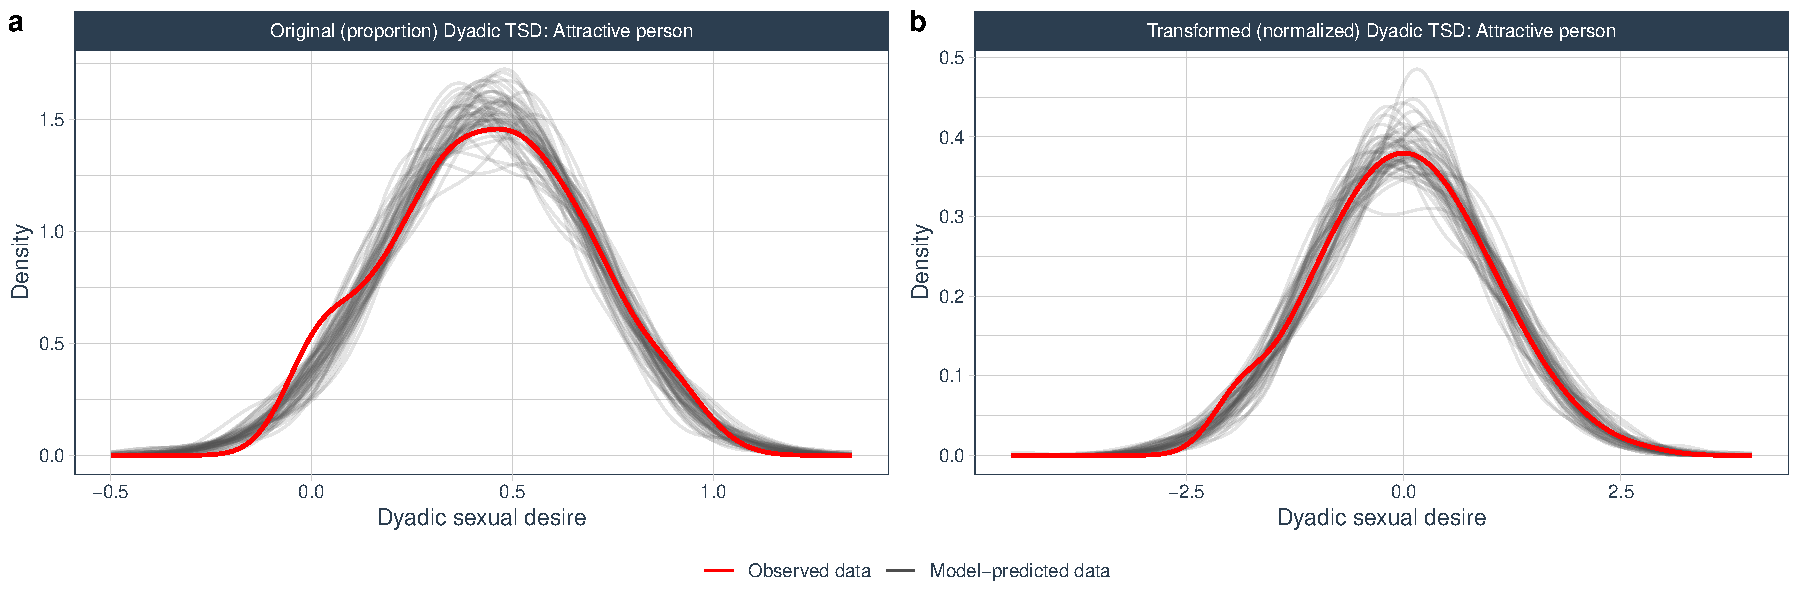
\includegraphics{Sexual_Desire_Arousal_V2_files/figure-latex/ppc-m1b-1.pdf}
\caption{\label{fig:ppc-m1b}Posterior predictive check. \textbf{(a)} Original (proportion) Solitary TSD; \textbf{(b)} Transformed (normalized) Solitary TSD. In both panels, red lines represent the observed data, and thin black lines represent 50 iterations of simulated data from each model.}
\end{figure}

\paragraph{\texorpdfstring{Table \ref{tab:tab-m1b}. Regression-type table for the interaction between \texttt{Relationship\ type}, and \texttt{Gender}}{Table \ref{tab:tab-m1b}. Regression-type table for the interaction between Relationship type, and Gender}}\label{table-reftabtab-m1b.-regression-type-table-for-the-interaction-between-relationship-type-and-gender}

This tables summarizes the results of the model.

\begin{Shaded}
\begin{Highlighting}[]
\FunctionTok{anova.sig}\NormalTok{(}\AttributeTok{model =}\NormalTok{ m1b\_norm, }\AttributeTok{custom\_caption =} \StringTok{"Effects of relationship type and gender on }
\StringTok{          Dyadic sexual desire: Attractive person"}\NormalTok{)}
\end{Highlighting}
\end{Shaded}

\begin{table}[H]
\centering
\caption{\label{tab:tab-m1b}Effects of relationship type and gender on 
          Dyadic sexual desire: Attractive person}
\centering
\resizebox{\ifdim\width>\linewidth\linewidth\else\width\fi}{!}{
\begin{threeparttable}
\begin{tabular}[t]{lcccl}
\toprule
Effect & $df$ & $F$ & $p$ & $\eta^2_G$\\
\midrule
Gender & 1, 319 & 29.85 & \textbf{< 0.0001} & 0.09\\
Relationship & 1, 319 & 8.20 & \textbf{0.004} & 0.03\\
Gender × Relationship & 1, 319 & 1.73 & 0.19 & 0.00\\
\bottomrule
\end{tabular}
\begin{tablenotes}[para]
\item \textit{Note: } 
\item Sexual desire was transformed using an ordered quantile 
                              normalization 
                              (\cite{petersonOrderedQuantileNormalization2020a}).
                              Results are type III ANOVA.
                              Gender = participants gender (women, men); 
                              Relationship = relationship type (stable, single).
                              As effect size, we used the generalized eta squared 
                              ($\eta^2_G$; see
                              \cite{bakemanRecommendedEffectSize2005}).
                              Significant effects are in bold.
\end{tablenotes}
\end{threeparttable}}
\end{table}

\paragraph{\texorpdfstring{\emph{Post-hoc} comparisons}{Post-hoc comparisons}}\label{post-hoc-comparisons-1}

Because the main effects of gender and relationship type, but not their interaction, are significant, we explored these effects using estimated marginal means.

\subparagraph{Table \ref{tab:tab-m1b-emm1}. Estimated marginal means and contrasts between participants' gender.}\label{table-reftabtab-m1b-emm1.-estimated-marginal-means-and-contrasts-between-participants-gender.}

Table of estimated marginal means and contrasts between genders. All estimated marginal means and contrasts were calculated using the \texttt{emmeans} function from the \texttt{emmeans} package \autocite{emmeanscit}.

\begin{Shaded}
\begin{Highlighting}[]
\NormalTok{emms.m1b1 }\OtherTok{\textless{}{-}} \FunctionTok{emmeans}\NormalTok{(m1b\_norm, }\SpecialCharTok{\textasciitilde{}}\NormalTok{ Gender)}

\NormalTok{emms.m1b1.tab }\OtherTok{\textless{}{-}} \FunctionTok{tibble}\NormalTok{(}\FunctionTok{data.frame}\NormalTok{(emms.m1b1))}

\NormalTok{t.m1b1 }\OtherTok{\textless{}{-}} \FunctionTok{contr.stars}\NormalTok{(emms.m1b1) }\SpecialCharTok{|\textgreater{}} 
  \FunctionTok{mutate}\NormalTok{(}\AttributeTok{p.value =} \FunctionTok{pval.lev}\NormalTok{(p.value))}

\FunctionTok{merge}\NormalTok{(emms.m1b1.tab, t.m1b1, }\AttributeTok{by =} \DecValTok{0}\NormalTok{, }\AttributeTok{all =} \ConstantTok{TRUE}\NormalTok{) }\SpecialCharTok{|\textgreater{}}
  \FunctionTok{select}\NormalTok{(}\SpecialCharTok{{-}}\FunctionTok{c}\NormalTok{(}\DecValTok{1}\NormalTok{,}\DecValTok{15}\NormalTok{)) }\SpecialCharTok{|\textgreater{}} 
  \FunctionTok{unite}\NormalTok{(Contrast, group1, group2, }\AttributeTok{sep =} \StringTok{" {-} "}\NormalTok{) }\SpecialCharTok{|\textgreater{}}
  \FunctionTok{mutate\_at}\NormalTok{(}\StringTok{"Contrast"}\NormalTok{, str\_replace\_all, }\StringTok{"NA {-} NA"}\NormalTok{, }\StringTok{" "}\NormalTok{) }\SpecialCharTok{|\textgreater{}} 
  \FunctionTok{kable}\NormalTok{(}\AttributeTok{digits =} \DecValTok{2}\NormalTok{,}
          \AttributeTok{booktabs =} \ConstantTok{TRUE}\NormalTok{,}
          \AttributeTok{align =} \FunctionTok{c}\NormalTok{(}\StringTok{"l"}\NormalTok{, }\FunctionTok{rep}\NormalTok{(}\StringTok{"c"}\NormalTok{, }\DecValTok{5}\NormalTok{), }\StringTok{"l"}\NormalTok{, }\FunctionTok{rep}\NormalTok{(}\StringTok{"c"}\NormalTok{, }\DecValTok{5}\NormalTok{)),}
          \AttributeTok{linesep =} \StringTok{""}\NormalTok{,}
          \AttributeTok{caption =} \StringTok{"Estimated marginal means and contrasts between participants\textquotesingle{} gender"}\NormalTok{,}
          \AttributeTok{col.names =} \FunctionTok{c}\NormalTok{(}\StringTok{"Gender"}\NormalTok{,}
                        \StringTok{"EMM"}\NormalTok{,}
                        \StringTok{"$SE$"}\NormalTok{,}
                        \StringTok{"$df$"}\NormalTok{,}
                        \StringTok{"$2.5}\SpecialCharTok{\textbackslash{}\textbackslash{}}\StringTok{\% CI$"}\NormalTok{,}
                        \StringTok{"$97.5}\SpecialCharTok{\textbackslash{}\textbackslash{}}\StringTok{\% CI$"}\NormalTok{,}
                        \StringTok{"Contrast"}\NormalTok{,}
                        \StringTok{"Difference"}\NormalTok{,}
                        \StringTok{"$SE$"}\NormalTok{,}
                        \StringTok{"$df$"}\NormalTok{,}
                        \StringTok{"$t$"}\NormalTok{,}
                        \StringTok{"$p$"}\NormalTok{),}
          \AttributeTok{escape =} \ConstantTok{FALSE}\NormalTok{) }\SpecialCharTok{|\textgreater{}}
  \FunctionTok{add\_header\_above}\NormalTok{(}\FunctionTok{c}\NormalTok{(}\StringTok{" "} \OtherTok{=} \DecValTok{6}\NormalTok{, }\StringTok{"Contrasts"} \OtherTok{=} \DecValTok{6}\NormalTok{)) }\SpecialCharTok{|\textgreater{}} 
  \FunctionTok{kable\_styling}\NormalTok{(}\AttributeTok{latex\_options =} \FunctionTok{c}\NormalTok{(}\StringTok{"HOLD\_position"}\NormalTok{, }\StringTok{"scale\_down"}\NormalTok{)) }\SpecialCharTok{|\textgreater{}}
  \FunctionTok{footnote}\NormalTok{(}\AttributeTok{general =} \StringTok{"Significant effects are in bold."}\NormalTok{,}
           \AttributeTok{threeparttable =} \ConstantTok{TRUE}\NormalTok{,}
           \AttributeTok{footnote\_as\_chunk =} \ConstantTok{TRUE}\NormalTok{,}
           \AttributeTok{escape =} \ConstantTok{FALSE}\NormalTok{)}
\end{Highlighting}
\end{Shaded}

\begin{table}[H]
\centering
\caption{\label{tab:tab-m1b-emm1}Estimated marginal means and contrasts between participants' gender}
\centering
\resizebox{\ifdim\width>\linewidth\linewidth\else\width\fi}{!}{
\begin{threeparttable}
\begin{tabular}[t]{lccccclccccc}
\toprule
\multicolumn{6}{c}{ } & \multicolumn{6}{c}{Contrasts} \\
\cmidrule(l{3pt}r{3pt}){7-12}
Gender & EMM & $SE$ & $df$ & $2.5\% CI$ & $97.5\% CI$ & Contrast & Difference & $SE$ & $df$ & $t$ & $p$\\
\midrule
Women & -0.22 & 0.07 & 319 & -0.36 & -0.09 & Women - Men & -0.57 & 0.1 & 319 & -5.46 & \textbf{< 0.0001}\\
Men & 0.35 & 0.08 & 319 & 0.19 & 0.50 &  &  &  &  &  & \\
\bottomrule
\end{tabular}
\begin{tablenotes}[para]
\item \textit{Note: } 
\item Significant effects are in bold.
\end{tablenotes}
\end{threeparttable}}
\end{table}

\subparagraph{Table \ref{tab:tab-m1b-emm2}. Estimated marginal means and contrasts between relationship status.}\label{table-reftabtab-m1b-emm2.-estimated-marginal-means-and-contrasts-between-relationship-status.}

Table of estimated marginal means and contrasts between relationship status. All estimated marginal means and contrasts were calculated using the \texttt{emmeans} function from the \texttt{emmeans} package \autocite{emmeanscit}.

\begin{Shaded}
\begin{Highlighting}[]
\NormalTok{emms.m1b2 }\OtherTok{\textless{}{-}} \FunctionTok{emmeans}\NormalTok{(m1b\_norm, }\SpecialCharTok{\textasciitilde{}}\NormalTok{ Relationship)}

\NormalTok{emms.m1b2.tab }\OtherTok{\textless{}{-}} \FunctionTok{tibble}\NormalTok{(}\FunctionTok{data.frame}\NormalTok{(emms.m1b2))}

\NormalTok{t.m1b2 }\OtherTok{\textless{}{-}} \FunctionTok{contr.stars}\NormalTok{(emms.m1b2) }\SpecialCharTok{|\textgreater{}} 
  \FunctionTok{mutate}\NormalTok{(}\AttributeTok{p.value =} \FunctionTok{pval.lev}\NormalTok{(p.value))}

\FunctionTok{merge}\NormalTok{(emms.m1b2.tab, t.m1b2, }\AttributeTok{by =} \DecValTok{0}\NormalTok{, }\AttributeTok{all =} \ConstantTok{TRUE}\NormalTok{) }\SpecialCharTok{|\textgreater{}}
  \FunctionTok{select}\NormalTok{(}\SpecialCharTok{{-}}\FunctionTok{c}\NormalTok{(}\DecValTok{1}\NormalTok{,}\DecValTok{15}\NormalTok{)) }\SpecialCharTok{|\textgreater{}} 
  \FunctionTok{unite}\NormalTok{(Contrast, group1, group2, }\AttributeTok{sep =} \StringTok{" {-} "}\NormalTok{) }\SpecialCharTok{|\textgreater{}}
  \FunctionTok{mutate\_at}\NormalTok{(}\StringTok{"Contrast"}\NormalTok{, str\_replace\_all, }\StringTok{"NA {-} NA"}\NormalTok{, }\StringTok{" "}\NormalTok{) }\SpecialCharTok{|\textgreater{}} 
  \FunctionTok{kable}\NormalTok{(}\AttributeTok{digits =} \DecValTok{2}\NormalTok{,}
          \AttributeTok{booktabs =} \ConstantTok{TRUE}\NormalTok{,}
          \AttributeTok{align =} \FunctionTok{c}\NormalTok{(}\StringTok{"l"}\NormalTok{, }\FunctionTok{rep}\NormalTok{(}\StringTok{"c"}\NormalTok{, }\DecValTok{5}\NormalTok{), }\StringTok{"l"}\NormalTok{, }\FunctionTok{rep}\NormalTok{(}\StringTok{"c"}\NormalTok{, }\DecValTok{5}\NormalTok{)),}
          \AttributeTok{linesep =} \StringTok{""}\NormalTok{,}
          \AttributeTok{caption =} \StringTok{"Estimated marginal means and contrasts between relationship status"}\NormalTok{,}
          \AttributeTok{col.names =} \FunctionTok{c}\NormalTok{(}\StringTok{"Relationship type"}\NormalTok{,}
                        \StringTok{"EMM"}\NormalTok{,}
                        \StringTok{"$SE$"}\NormalTok{,}
                        \StringTok{"$df$"}\NormalTok{,}
                        \StringTok{"$2.5}\SpecialCharTok{\textbackslash{}\textbackslash{}}\StringTok{\% CI$"}\NormalTok{,}
                        \StringTok{"$97.5}\SpecialCharTok{\textbackslash{}\textbackslash{}}\StringTok{\% CI$"}\NormalTok{,}
                        \StringTok{"Contrast"}\NormalTok{,}
                        \StringTok{"Difference"}\NormalTok{,}
                        \StringTok{"$SE$"}\NormalTok{,}
                        \StringTok{"$df$"}\NormalTok{,}
                        \StringTok{"$t$"}\NormalTok{,}
                        \StringTok{"$p$"}\NormalTok{),}
          \AttributeTok{escape =} \ConstantTok{FALSE}\NormalTok{) }\SpecialCharTok{|\textgreater{}}
  \FunctionTok{add\_header\_above}\NormalTok{(}\FunctionTok{c}\NormalTok{(}\StringTok{" "} \OtherTok{=} \DecValTok{6}\NormalTok{, }\StringTok{"Contrasts"} \OtherTok{=} \DecValTok{6}\NormalTok{)) }\SpecialCharTok{|\textgreater{}} 
  \FunctionTok{kable\_styling}\NormalTok{(}\AttributeTok{latex\_options =} \FunctionTok{c}\NormalTok{(}\StringTok{"HOLD\_position"}\NormalTok{, }\StringTok{"scale\_down"}\NormalTok{)) }\SpecialCharTok{|\textgreater{}}
  \FunctionTok{footnote}\NormalTok{(}\AttributeTok{general =} \StringTok{"Significant effects are in bold."}\NormalTok{,}
           \AttributeTok{threeparttable =} \ConstantTok{TRUE}\NormalTok{,}
           \AttributeTok{footnote\_as\_chunk =} \ConstantTok{TRUE}\NormalTok{,}
           \AttributeTok{escape =} \ConstantTok{FALSE}\NormalTok{)}
\end{Highlighting}
\end{Shaded}

\begin{table}[H]
\centering
\caption{\label{tab:tab-m1b-emm2}Estimated marginal means and contrasts between relationship status}
\centering
\resizebox{\ifdim\width>\linewidth\linewidth\else\width\fi}{!}{
\begin{threeparttable}
\begin{tabular}[t]{lccccclccccc}
\toprule
\multicolumn{6}{c}{ } & \multicolumn{6}{c}{Contrasts} \\
\cmidrule(l{3pt}r{3pt}){7-12}
Relationship type & EMM & $SE$ & $df$ & $2.5\% CI$ & $97.5\% CI$ & Contrast & Difference & $SE$ & $df$ & $t$ & $p$\\
\midrule
Stable & -0.09 & 0.07 & 319 & -0.22 & 0.05 & Stable - Single & -0.3 & 0.1 & 319 & -2.86 & \textbf{0.0045}\\
Single & 0.21 & 0.08 & 319 & 0.06 & 0.36 &  &  &  &  &  & \\
\bottomrule
\end{tabular}
\begin{tablenotes}[para]
\item \textit{Note: } 
\item Significant effects are in bold.
\end{tablenotes}
\end{threeparttable}}
\end{table}

\subparagraph{Table \ref{tab:tab-m1b-emm3}. Estimated marginal means and contrasts between gender by relationship status.}\label{table-reftabtab-m1b-emm3.-estimated-marginal-means-and-contrasts-between-gender-by-relationship-status.}

Table of estimated marginal means and contrasts between gender by relationship status. All estimated marginal means and contrasts were calculated using the \texttt{emmeans} function from the \texttt{emmeans} package \autocite{emmeanscit}.

\begin{Shaded}
\begin{Highlighting}[]
\NormalTok{emms.m1b3 }\OtherTok{\textless{}{-}} \FunctionTok{emmeans}\NormalTok{(m1b\_norm, }\SpecialCharTok{\textasciitilde{}}\NormalTok{ Gender }\SpecialCharTok{|}\NormalTok{ Relationship)}

\NormalTok{emms.m1b3.tab }\OtherTok{\textless{}{-}} \FunctionTok{tibble}\NormalTok{(}\FunctionTok{data.frame}\NormalTok{(emms.m1b3))}

\NormalTok{t.m1b3 }\OtherTok{\textless{}{-}} \FunctionTok{contr.stars}\NormalTok{(emms.m1b3) }\SpecialCharTok{|\textgreater{}} 
  \FunctionTok{mutate}\NormalTok{(}\AttributeTok{p.value =} \FunctionTok{pval.lev}\NormalTok{(p.value))}

\NormalTok{t.m1b3.f }\OtherTok{\textless{}{-}}\NormalTok{ t.m1b3 }\SpecialCharTok{|\textgreater{}} 
  \FunctionTok{insertRows}\NormalTok{(}\DecValTok{2}\NormalTok{, }\AttributeTok{new =} \ConstantTok{NA}\NormalTok{) }\SpecialCharTok{|\textgreater{}}
\FunctionTok{insertRows}\NormalTok{(}\DecValTok{4}\NormalTok{, }\AttributeTok{new =} \ConstantTok{NA}\NormalTok{)}

\FunctionTok{merge}\NormalTok{(emms.m1b3.tab, t.m1b3.f, }\AttributeTok{by =} \DecValTok{0}\NormalTok{, }\AttributeTok{all =} \ConstantTok{TRUE}\NormalTok{) }\SpecialCharTok{|\textgreater{}}
  \FunctionTok{select}\NormalTok{(}\SpecialCharTok{{-}}\FunctionTok{c}\NormalTok{(}\DecValTok{1}\NormalTok{,}\DecValTok{3}\NormalTok{,}\DecValTok{11}\NormalTok{,}\DecValTok{17}\NormalTok{)) }\SpecialCharTok{|\textgreater{}} 
  \FunctionTok{drop\_na}\NormalTok{(Gender) }\SpecialCharTok{|\textgreater{}} 
  \FunctionTok{unite}\NormalTok{(Contrast, group1, group2, }\AttributeTok{sep =} \StringTok{" {-} "}\NormalTok{) }\SpecialCharTok{|\textgreater{}}
  \FunctionTok{mutate\_at}\NormalTok{(}\StringTok{"Contrast"}\NormalTok{, str\_replace\_all, }\StringTok{"NA {-} NA"}\NormalTok{, }\StringTok{""}\NormalTok{) }\SpecialCharTok{|\textgreater{}} 
  \FunctionTok{kable}\NormalTok{(}\AttributeTok{digits =} \DecValTok{2}\NormalTok{,}
          \AttributeTok{booktabs =} \ConstantTok{TRUE}\NormalTok{,}
          \AttributeTok{align =} \FunctionTok{c}\NormalTok{(}\StringTok{"l"}\NormalTok{, }\StringTok{"l"}\NormalTok{, }\FunctionTok{rep}\NormalTok{(}\StringTok{"c"}\NormalTok{, }\DecValTok{5}\NormalTok{), }\StringTok{"l"}\NormalTok{, }\FunctionTok{rep}\NormalTok{(}\StringTok{"c"}\NormalTok{, }\DecValTok{5}\NormalTok{)),}
          \AttributeTok{linesep =} \StringTok{""}\NormalTok{,}
          \AttributeTok{caption =} \StringTok{"Estimated marginal means and contrasts between gender by }
\StringTok{                    relationship status"}\NormalTok{,}
          \AttributeTok{col.names =} \FunctionTok{c}\NormalTok{(}\StringTok{"Gender"}\NormalTok{,}
                        \CommentTok{\#"Relationship",}
                        \StringTok{"EMM"}\NormalTok{,}
                        \StringTok{"$SE$"}\NormalTok{,}
                        \StringTok{"$df$"}\NormalTok{,}
                        \StringTok{"$2.5}\SpecialCharTok{\textbackslash{}\textbackslash{}}\StringTok{\% CI$"}\NormalTok{,}
                        \StringTok{"$97.5}\SpecialCharTok{\textbackslash{}\textbackslash{}}\StringTok{\% CI$"}\NormalTok{,}
                        \StringTok{"Contrast"}\NormalTok{,}
                        \StringTok{"Difference"}\NormalTok{,}
                        \StringTok{"$SE$"}\NormalTok{,}
                        \StringTok{"$df$"}\NormalTok{,}
                        \StringTok{"$t$"}\NormalTok{,}
                        \StringTok{"$p$"}\NormalTok{),}
          \AttributeTok{escape =} \ConstantTok{FALSE}\NormalTok{) }\SpecialCharTok{|\textgreater{}}
  \FunctionTok{pack\_rows}\NormalTok{(}\AttributeTok{group\_label =} \StringTok{"Relationship status: Stable"}\NormalTok{,}
            \AttributeTok{start\_row =} \DecValTok{1}\NormalTok{,}
            \AttributeTok{end\_row =} \DecValTok{2}\NormalTok{,}
            \AttributeTok{hline\_before =} \ConstantTok{FALSE}\NormalTok{,}
            \AttributeTok{bold =} \ConstantTok{TRUE}\NormalTok{) }\SpecialCharTok{|\textgreater{}}
  \FunctionTok{pack\_rows}\NormalTok{(}\AttributeTok{group\_label =} \StringTok{"Relationship status: Single"}\NormalTok{,}
            \AttributeTok{start\_row =} \DecValTok{3}\NormalTok{,}
            \AttributeTok{end\_row =} \DecValTok{4}\NormalTok{,}
            \AttributeTok{hline\_before =} \ConstantTok{TRUE}\NormalTok{,}
            \AttributeTok{bold =} \ConstantTok{TRUE}\NormalTok{) }\SpecialCharTok{|\textgreater{}}
  \FunctionTok{add\_header\_above}\NormalTok{(}\FunctionTok{c}\NormalTok{(}\StringTok{" "} \OtherTok{=} \DecValTok{6}\NormalTok{, }\StringTok{"Contrasts"} \OtherTok{=} \DecValTok{6}\NormalTok{)) }\SpecialCharTok{|\textgreater{}} 
  \FunctionTok{kable\_styling}\NormalTok{(}\AttributeTok{latex\_options =} \FunctionTok{c}\NormalTok{(}\StringTok{"HOLD\_position"}\NormalTok{, }\StringTok{"scale\_down"}\NormalTok{)) }\SpecialCharTok{|\textgreater{}}
  \FunctionTok{footnote}\NormalTok{(}\AttributeTok{general =} \StringTok{"Significant effects are in bold."}\NormalTok{,}
           \AttributeTok{threeparttable =} \ConstantTok{TRUE}\NormalTok{,}
           \AttributeTok{footnote\_as\_chunk =} \ConstantTok{TRUE}\NormalTok{,}
           \AttributeTok{escape =} \ConstantTok{FALSE}\NormalTok{)}
\end{Highlighting}
\end{Shaded}

\begin{table}[H]
\centering
\caption{\label{tab:tab-m1b-emm3}Estimated marginal means and contrasts between gender by 
                    relationship status}
\centering
\resizebox{\ifdim\width>\linewidth\linewidth\else\width\fi}{!}{
\begin{threeparttable}
\begin{tabular}[t]{llccccclcccc}
\toprule
\multicolumn{6}{c}{ } & \multicolumn{6}{c}{Contrasts} \\
\cmidrule(l{3pt}r{3pt}){7-12}
Gender & EMM & $SE$ & $df$ & $2.5\% CI$ & $97.5\% CI$ & Contrast & Difference & $SE$ & $df$ & $t$ & $p$\\
\midrule
\addlinespace[0.3em]
\multicolumn{12}{l}{\textbf{Relationship status: Stable}}\\
\hspace{1em}Women & -0.44 & 0.09 & 319 & -0.62 & -0.26 & Women - Men & -0.71 & 0.14 & 319 & -5.00 & \textbf{< 0.0001}\\
\hspace{1em}Men & 0.27 & 0.11 & 319 & 0.05 & 0.48 &  &  &  &  &  & \\
\addlinespace[0.3em]
\hline
\multicolumn{12}{l}{\textbf{Relationship status: Single}}\\
\hspace{1em}Women & 0.00 & 0.10 & 319 & -0.21 & 0.20 & Women - Men & -0.43 & 0.15 & 319 & -2.82 & \textbf{0.0051}\\
\hspace{1em}Men & 0.43 & 0.11 & 319 & 0.21 & 0.65 &  &  &  &  &  & \\
\bottomrule
\end{tabular}
\begin{tablenotes}[para]
\item \textit{Note: } 
\item Significant effects are in bold.
\end{tablenotes}
\end{threeparttable}}
\end{table}

\paragraph{Figure \ref{fig:fig-h1b}. Differences among the three dimensions of sexual desire}\label{figure-reffigfig-h1b.-differences-among-the-three-dimensions-of-sexual-desire}

This figure summarizes the results of hypothesis 1b.

\begin{Shaded}
\begin{Highlighting}[]
\CommentTok{\# Gender main effect}
\NormalTok{h1b1 }\OtherTok{\textless{}{-}} \FunctionTok{ggplot}\NormalTok{(dat\_m1, }\FunctionTok{aes}\NormalTok{(}\AttributeTok{x =}\NormalTok{ Gender, }\AttributeTok{y =} \StringTok{\textasciigrave{}}\AttributeTok{Dyadic sexual desire: Attractive person (normalized)}\StringTok{\textasciigrave{}}\NormalTok{, }
                          \AttributeTok{color =}\NormalTok{ Gender)) }\SpecialCharTok{+}
  \FunctionTok{geom\_violin}\NormalTok{(}\AttributeTok{trim =} \ConstantTok{FALSE}\NormalTok{) }\SpecialCharTok{+}
  \FunctionTok{geom\_jitter}\NormalTok{(}\AttributeTok{alpha =} \FloatTok{0.3}\NormalTok{, }\AttributeTok{width =} \FloatTok{0.1}\NormalTok{) }\SpecialCharTok{+}
  \FunctionTok{scale\_color\_manual}\NormalTok{(}\AttributeTok{values =}\NormalTok{ color.Gender) }\SpecialCharTok{+}
  \FunctionTok{scale\_fill\_manual}\NormalTok{(}\AttributeTok{values =}\NormalTok{ color.Gender) }\SpecialCharTok{+}
  \FunctionTok{geom\_errorbar}\NormalTok{(}\AttributeTok{data =}\NormalTok{ emms.m1b1.tab }\SpecialCharTok{|\textgreater{}} 
                  \FunctionTok{rename}\NormalTok{(}\StringTok{\textquotesingle{}Dyadic sexual desire: Attractive person (normalized)\textquotesingle{}} \OtherTok{=}\NormalTok{ emmean),}
                \AttributeTok{mapping =} \FunctionTok{aes}\NormalTok{(}\AttributeTok{ymin =}\NormalTok{ lower.CL, }\AttributeTok{ymax =}\NormalTok{ upper.CL), }
                \AttributeTok{colour =} \StringTok{"black"}\NormalTok{, }\AttributeTok{width =} \FloatTok{0.1}\NormalTok{) }\SpecialCharTok{+}
  \FunctionTok{geom\_point}\NormalTok{(}\AttributeTok{data =}\NormalTok{ emms.m1b1.tab }\SpecialCharTok{|\textgreater{}} 
                  \FunctionTok{rename}\NormalTok{(}\StringTok{\textquotesingle{}Dyadic sexual desire: Attractive person (normalized)\textquotesingle{}} \OtherTok{=}\NormalTok{ emmean), }
             \AttributeTok{position =} \FunctionTok{position\_dodge}\NormalTok{(}\FloatTok{0.1}\NormalTok{), }
             \AttributeTok{shape =} \DecValTok{21}\NormalTok{, }\AttributeTok{size =} \DecValTok{3}\NormalTok{,}
             \AttributeTok{color =} \StringTok{"black"}\NormalTok{, }\AttributeTok{fill =} \StringTok{"white"}\NormalTok{) }\SpecialCharTok{+}
  \FunctionTok{stat\_pvalue\_manual}\NormalTok{(t.m1b1, }
                     \AttributeTok{label =} \StringTok{"p.signif"}\NormalTok{, }
                     \AttributeTok{y.position =} \FloatTok{3.5}\NormalTok{, }
                     \AttributeTok{tip.length =} \DecValTok{0}\NormalTok{) }\SpecialCharTok{+}
  \FunctionTok{guides}\NormalTok{(}\AttributeTok{color =} \StringTok{"none"}\NormalTok{) }\SpecialCharTok{+}
  \FunctionTok{theme\_tq}\NormalTok{()}

\CommentTok{\# Relationship main effect}
\NormalTok{h1b2 }\OtherTok{\textless{}{-}} \FunctionTok{ggplot}\NormalTok{(dat\_m1, }\FunctionTok{aes}\NormalTok{(}\AttributeTok{x =}\NormalTok{ Relationship, }\AttributeTok{y =} \StringTok{\textasciigrave{}}\AttributeTok{Dyadic sexual desire: Attractive person (normalized)}\StringTok{\textasciigrave{}}\NormalTok{, }
                          \AttributeTok{color =}\NormalTok{ Relationship)) }\SpecialCharTok{+}
  \FunctionTok{geom\_violin}\NormalTok{(}\AttributeTok{trim =} \ConstantTok{FALSE}\NormalTok{) }\SpecialCharTok{+}
  \FunctionTok{geom\_jitter}\NormalTok{(}\AttributeTok{alpha =} \FloatTok{0.3}\NormalTok{, }\AttributeTok{width =} \FloatTok{0.1}\NormalTok{) }\SpecialCharTok{+}
  \FunctionTok{scale\_color\_manual}\NormalTok{(}\AttributeTok{values =}\NormalTok{ color.Relationship) }\SpecialCharTok{+}
  \FunctionTok{scale\_fill\_manual}\NormalTok{(}\AttributeTok{values =}\NormalTok{ color.Relationship) }\SpecialCharTok{+}
  \FunctionTok{geom\_errorbar}\NormalTok{(}\AttributeTok{data =}\NormalTok{ emms.m1b2.tab }\SpecialCharTok{|\textgreater{}} 
                  \FunctionTok{rename}\NormalTok{(}\StringTok{\textquotesingle{}Dyadic sexual desire: Attractive person (normalized)\textquotesingle{}} \OtherTok{=}\NormalTok{ emmean),}
                \AttributeTok{mapping =} \FunctionTok{aes}\NormalTok{(}\AttributeTok{ymin =}\NormalTok{ lower.CL, }\AttributeTok{ymax =}\NormalTok{ upper.CL), }
                \AttributeTok{colour =} \StringTok{"black"}\NormalTok{, }\AttributeTok{width =} \FloatTok{0.1}\NormalTok{) }\SpecialCharTok{+}
  \FunctionTok{geom\_point}\NormalTok{(}\AttributeTok{data =}\NormalTok{ emms.m1b2.tab }\SpecialCharTok{|\textgreater{}} 
                  \FunctionTok{rename}\NormalTok{(}\StringTok{\textquotesingle{}Dyadic sexual desire: Attractive person (normalized)\textquotesingle{}} \OtherTok{=}\NormalTok{ emmean), }
             \AttributeTok{position =} \FunctionTok{position\_dodge}\NormalTok{(}\FloatTok{0.1}\NormalTok{), }
             \AttributeTok{shape =} \DecValTok{21}\NormalTok{, }\AttributeTok{size =} \DecValTok{3}\NormalTok{,}
             \AttributeTok{color =} \StringTok{"black"}\NormalTok{, }\AttributeTok{fill =} \StringTok{"white"}\NormalTok{) }\SpecialCharTok{+}
  \FunctionTok{stat\_pvalue\_manual}\NormalTok{(t.m1b2, }
                     \AttributeTok{label =} \StringTok{"p.signif"}\NormalTok{, }
                     \AttributeTok{y.position =} \FloatTok{3.5}\NormalTok{, }
                     \AttributeTok{tip.length =} \DecValTok{0}\NormalTok{) }\SpecialCharTok{+}
  \FunctionTok{guides}\NormalTok{(}\AttributeTok{color =} \StringTok{"none"}\NormalTok{) }\SpecialCharTok{+}
  \FunctionTok{theme\_tq}\NormalTok{()}

\CommentTok{\# Relationship × Gender interaction}
\NormalTok{h1b3 }\OtherTok{\textless{}{-}} \FunctionTok{ggplot}\NormalTok{(dat\_m1, }\FunctionTok{aes}\NormalTok{(}\AttributeTok{x =}\NormalTok{ Gender, }\AttributeTok{y =} \StringTok{\textasciigrave{}}\AttributeTok{Dyadic sexual desire: Attractive person (normalized)}\StringTok{\textasciigrave{}}\NormalTok{, }
                           \AttributeTok{color =}\NormalTok{ Gender)) }\SpecialCharTok{+}
  \FunctionTok{geom\_violin}\NormalTok{(}\AttributeTok{trim =} \ConstantTok{FALSE}\NormalTok{) }\SpecialCharTok{+}
  \FunctionTok{geom\_jitter}\NormalTok{(}\AttributeTok{alpha =} \FloatTok{0.3}\NormalTok{, }\AttributeTok{width =} \FloatTok{0.1}\NormalTok{) }\SpecialCharTok{+}
  \FunctionTok{scale\_color\_manual}\NormalTok{(}\AttributeTok{values =}\NormalTok{ color.Gender) }\SpecialCharTok{+}
  \FunctionTok{scale\_fill\_manual}\NormalTok{(}\AttributeTok{values =}\NormalTok{ color.Gender) }\SpecialCharTok{+}
  \FunctionTok{facet\_wrap}\NormalTok{(}\SpecialCharTok{\textasciitilde{}}\NormalTok{Relationship) }\SpecialCharTok{+}
  \FunctionTok{geom\_errorbar}\NormalTok{(}\AttributeTok{data =}\NormalTok{ emms.m1b3.tab }\SpecialCharTok{|\textgreater{}} 
                  \FunctionTok{rename}\NormalTok{(}\StringTok{\textquotesingle{}Dyadic sexual desire: Attractive person (normalized)\textquotesingle{}} \OtherTok{=}\NormalTok{ emmean), }
                \AttributeTok{mapping =} \FunctionTok{aes}\NormalTok{(}\AttributeTok{ymin =}\NormalTok{ lower.CL, }\AttributeTok{ymax =}\NormalTok{ upper.CL), }
                \AttributeTok{colour =} \StringTok{"black"}\NormalTok{, }\AttributeTok{width =} \FloatTok{0.1}\NormalTok{) }\SpecialCharTok{+}
  \FunctionTok{geom\_point}\NormalTok{(}\AttributeTok{data =}\NormalTok{ emms.m1b3.tab}\SpecialCharTok{|\textgreater{}} 
                  \FunctionTok{rename}\NormalTok{(}\StringTok{\textquotesingle{}Dyadic sexual desire: Attractive person (normalized)\textquotesingle{}} \OtherTok{=}\NormalTok{ emmean), }
             \AttributeTok{position =} \FunctionTok{position\_dodge}\NormalTok{(}\FloatTok{0.1}\NormalTok{), }
             \AttributeTok{shape =} \DecValTok{21}\NormalTok{, }\AttributeTok{size =} \DecValTok{3}\NormalTok{,}
             \AttributeTok{color =} \StringTok{"black"}\NormalTok{, }\AttributeTok{fill =} \StringTok{"white"}\NormalTok{) }\SpecialCharTok{+}
  \FunctionTok{stat\_pvalue\_manual}\NormalTok{(t.m1b3, }
                     \AttributeTok{label =} \StringTok{"p.signif"}\NormalTok{, }
                     \AttributeTok{y.position =} \FloatTok{3.5}\NormalTok{, }
                     \AttributeTok{tip.length =} \DecValTok{0}\NormalTok{) }\SpecialCharTok{+}
  \FunctionTok{guides}\NormalTok{(}\AttributeTok{color =} \StringTok{"none"}\NormalTok{) }\SpecialCharTok{+}
  \FunctionTok{theme\_tq}\NormalTok{()}

\CommentTok{\# Full figure for hypothesis 1 (a, b and c)}
\NormalTok{p1b }\OtherTok{\textless{}{-}} \FunctionTok{ggarrange}\NormalTok{(h1b1, h1b2, h1b3,}
                 \AttributeTok{ncol =} \DecValTok{3}\NormalTok{,}
                 \AttributeTok{labels =} \StringTok{"auto"}\NormalTok{,}
                 \AttributeTok{widths =} \FunctionTok{c}\NormalTok{(}\DecValTok{1}\NormalTok{,}\DecValTok{1}\NormalTok{,}\FloatTok{1.5}\NormalTok{))}
\NormalTok{p1b}
\end{Highlighting}
\end{Shaded}

\begin{figure}
\centering
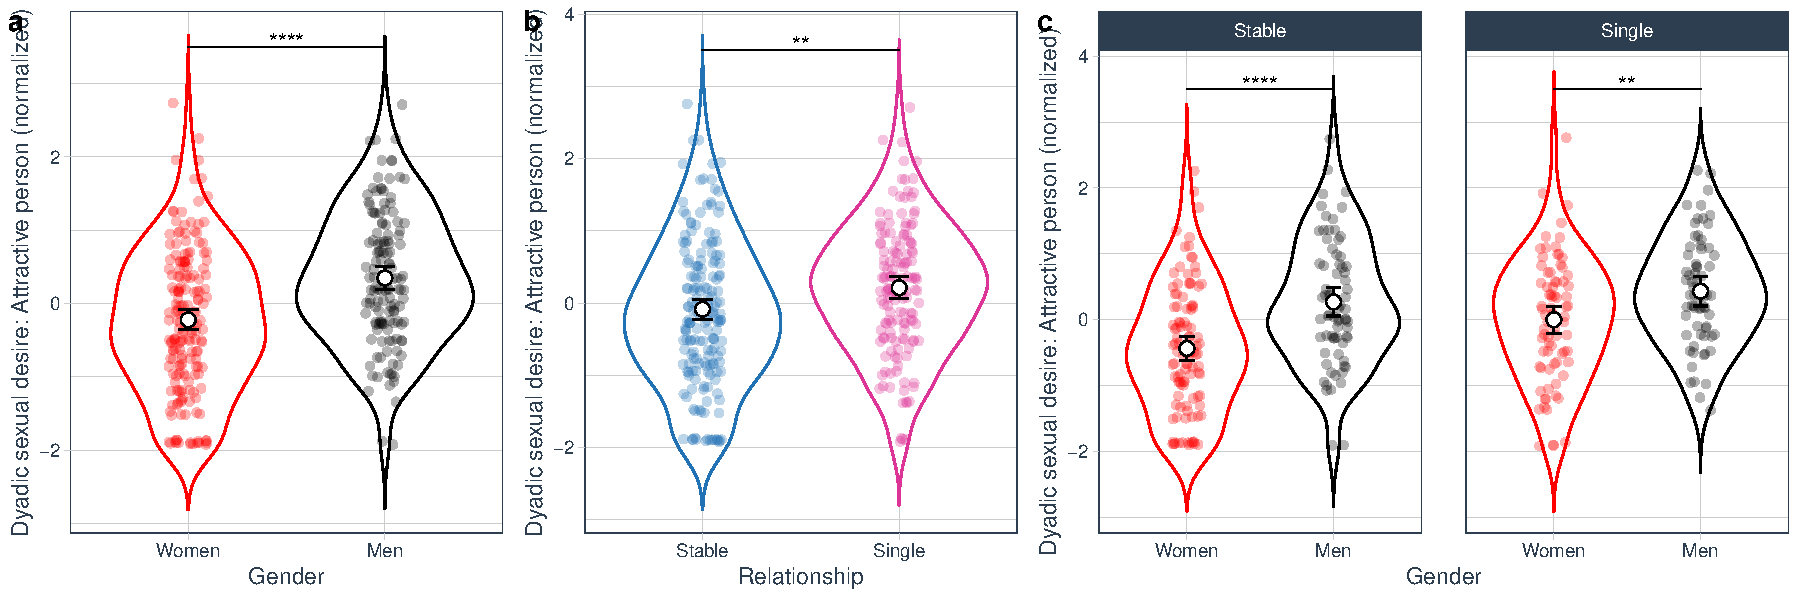
\includegraphics{Sexual_Desire_Arousal_V2_files/figure-latex/fig-h1b-1.pdf}
\caption{\label{fig:fig-h1b}Effects of gender and relationship type on Dyadic sexual desire: Attractive person. Dyadic sexual desire: Attractive person was transformed using ordered quantile normalization \autocite{petersonOrderedQuantileNormalization2020a}. \textbf{(a)} Simple comparison between sexual desire by gender (for detailed results, see Table \ref{tab:tab-m1b-emm1}); \textbf{(b)} Simple comparison between relationship status levels (for detailed results, see Table \ref{tab:tab-m1b-emm2}); \textbf{(c)} Interaction between relationship type and relationship status (see Table \ref{tab:tab-m1b}; for detailed results, see Table \ref{tab:tab-m1b-emm3}). White dots and black bars represent estimated marginal means and 95\% CI. In all cases, significant effects are represented with lines and stars: *\emph{p} \textless{} 0.05, **\emph{p} \textless{} 0.01, ***\emph{p} \textless{} 0.001, ****\emph{p} \textless{} 0.0001.}
\end{figure}

\subsubsection{Hypothesis 1c: Solitary TSD}\label{hypothesis1c}

\paragraph{Model the effects of relationship type and gender on Solitary TSD}\label{model-the-effects-of-relationship-type-and-gender-on-solitary-tsd-2}

We fitted models with both the original (proportion; \texttt{m1c\_prop}) and transformed (normalized; \texttt{m1c\_norm}) TSD scores, and performed posterior predictive checks (PPCs). As shown elsewhere \autocite[e.g.,][]{gabryVisualizationBayesianWorkflow2019}, if simulated data from one model are more similar to the observed outcome, that model is likely to be preferred.

\begin{Shaded}
\begin{Highlighting}[]
\FunctionTok{options}\NormalTok{(}\AttributeTok{contrasts =} \FunctionTok{c}\NormalTok{(}\StringTok{"contr.sum"}\NormalTok{,}\StringTok{"contr.poly"}\NormalTok{))}
\NormalTok{m1c\_prop }\OtherTok{\textless{}{-}} \FunctionTok{lm}\NormalTok{(}\StringTok{\textasciigrave{}}\AttributeTok{Dyadic sexual desire: Partner (proportion)}\StringTok{\textasciigrave{}} \SpecialCharTok{\textasciitilde{}}\NormalTok{ Gender }\SpecialCharTok{*}\NormalTok{ Relationship,}
            \AttributeTok{data =}\NormalTok{ dat\_m1)}

\NormalTok{m1c\_norm }\OtherTok{\textless{}{-}} \FunctionTok{lm}\NormalTok{(}\StringTok{\textasciigrave{}}\AttributeTok{Dyadic sexual desire: Partner (normalized)}\StringTok{\textasciigrave{}} \SpecialCharTok{\textasciitilde{}}\NormalTok{ Gender }\SpecialCharTok{*}\NormalTok{ Relationship,}
           \AttributeTok{data =}\NormalTok{ dat\_m1)}
\end{Highlighting}
\end{Shaded}

\subparagraph{Figure \ref{fig:ppc-m1c}: Posterior predictive checks (PPCs) for Hypothesis 1c.}\label{figure-reffigppc-m1c-posterior-predictive-checks-ppcs-for-hypothesis-1c.}

PPCs were performed using the \texttt{check\_model} function from the \texttt{performance} package \autocite{ludecke2021}, and reported in Fig. \ref{fig:ppc-m1c}. Simulated data from the normalized Solitary TSD model (Fig. \ref{fig:ppc-m1c}b) are more similar to the observed outcome, so this model is preferred.

\begin{Shaded}
\begin{Highlighting}[]
\NormalTok{ppc\_m1c }\OtherTok{\textless{}{-}} \FunctionTok{ggarrange}\NormalTok{(}\FunctionTok{plot}\NormalTok{(}\FunctionTok{check\_model}\NormalTok{(m1c\_prop, }
                                      \AttributeTok{panel =} \ConstantTok{FALSE}\NormalTok{,}
                                      \AttributeTok{check =} \StringTok{"pp\_check"}\NormalTok{)}\SpecialCharTok{$}\NormalTok{PP\_CHECK,}
                          \AttributeTok{colors =} \FunctionTok{c}\NormalTok{(}\StringTok{"red"}\NormalTok{, }\StringTok{"grey30"}\NormalTok{)) }\SpecialCharTok{+}
                       \FunctionTok{labs}\NormalTok{(}\AttributeTok{title =} \ConstantTok{NULL}\NormalTok{, }\AttributeTok{subtitle =} \ConstantTok{NULL}\NormalTok{) }\SpecialCharTok{+}
                       \FunctionTok{theme\_tq}\NormalTok{() }\SpecialCharTok{+}
                       \FunctionTok{facet\_wrap}\NormalTok{(}\SpecialCharTok{\textasciitilde{}} \DecValTok{1}\NormalTok{, }\AttributeTok{labeller =} \FunctionTok{as\_labeller}\NormalTok{(}\FunctionTok{c}\NormalTok{(}
                         \StringTok{"1"} \OtherTok{=} \StringTok{"Original (proportion) Dyadic TSD: Partner"}\NormalTok{))),}
                     \FunctionTok{plot}\NormalTok{(}\FunctionTok{check\_model}\NormalTok{(m1c\_norm, }
                                      \AttributeTok{panel =} \ConstantTok{FALSE}\NormalTok{,}
                                      \AttributeTok{check =} \StringTok{"pp\_check"}\NormalTok{)}\SpecialCharTok{$}\NormalTok{PP\_CHECK,}
                          \AttributeTok{colors =} \FunctionTok{c}\NormalTok{(}\StringTok{"red"}\NormalTok{, }\StringTok{"grey30"}\NormalTok{)) }\SpecialCharTok{+}
                       \FunctionTok{labs}\NormalTok{(}\AttributeTok{title =} \ConstantTok{NULL}\NormalTok{, }\AttributeTok{subtitle =} \ConstantTok{NULL}\NormalTok{) }\SpecialCharTok{+}
                       \FunctionTok{theme\_tq}\NormalTok{() }\SpecialCharTok{+}
                       \FunctionTok{facet\_wrap}\NormalTok{(}\SpecialCharTok{\textasciitilde{}} \DecValTok{1}\NormalTok{, }\AttributeTok{labeller =} \FunctionTok{as\_labeller}\NormalTok{(}\FunctionTok{c}\NormalTok{(}
                         \StringTok{"1"} \OtherTok{=} \StringTok{"Transformed (normalized) Dyadic TSD: Partner"}\NormalTok{))),}
                     \AttributeTok{labels =} \StringTok{"auto"}\NormalTok{,}
                     \AttributeTok{common.legend =} \ConstantTok{TRUE}\NormalTok{,}
                     \AttributeTok{legend =} \StringTok{"bottom"}\NormalTok{)}
\NormalTok{ppc\_m1c}
\end{Highlighting}
\end{Shaded}

\begin{figure}
\centering
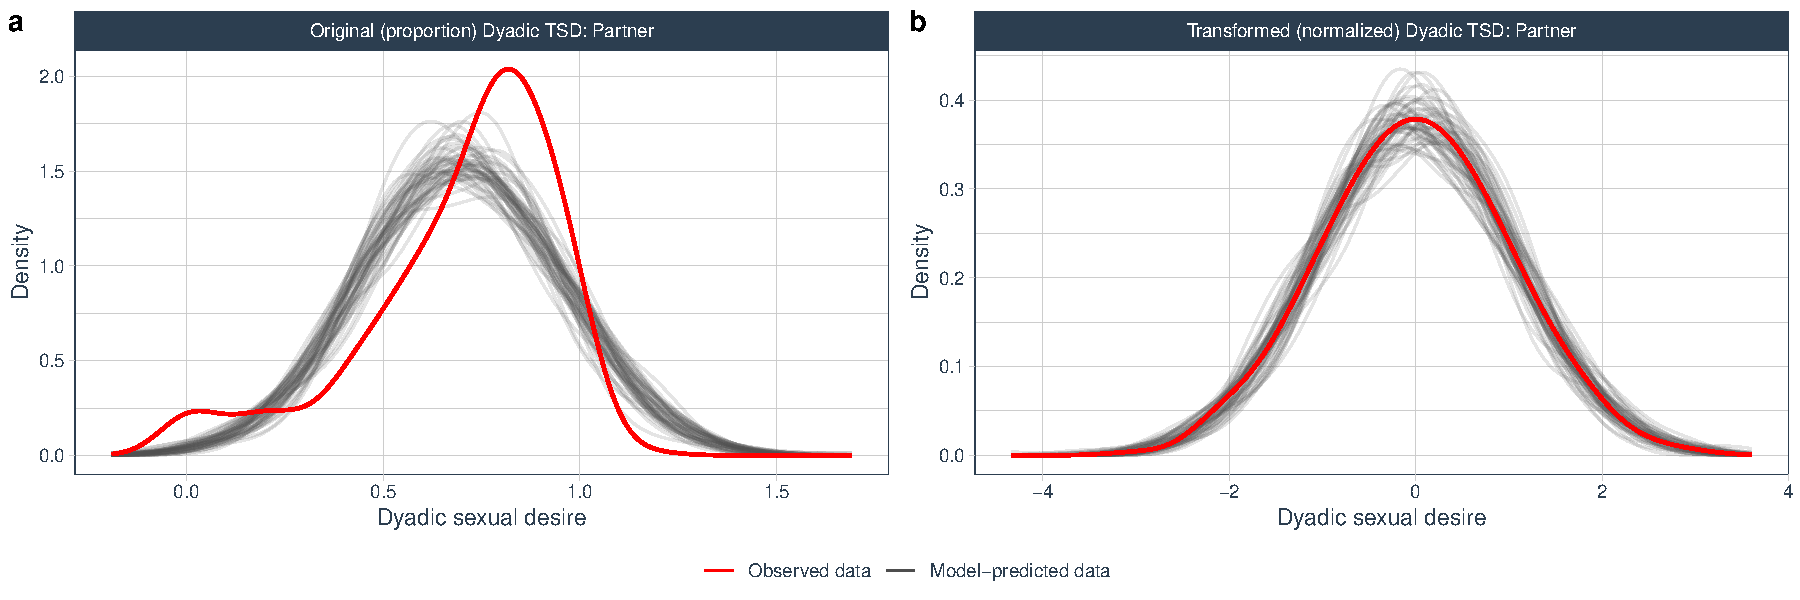
\includegraphics{Sexual_Desire_Arousal_V2_files/figure-latex/ppc-m1c-1.pdf}
\caption{\label{fig:ppc-m1c}Posterior predictive check. \textbf{(a)} Original (proportion) Solitary TSD; \textbf{(b)} Transformed (normalized) Solitary TSD. In both panels, red lines represent the observed data, and thin black lines represent 50 iterations of simulated data from each model.}
\end{figure}

\paragraph{\texorpdfstring{Table \ref{tab:tab-m1c}. Regression-type table for the interaction between \texttt{Relationship\ type}, and \texttt{Gender}}{Table \ref{tab:tab-m1c}. Regression-type table for the interaction between Relationship type, and Gender}}\label{table-reftabtab-m1c.-regression-type-table-for-the-interaction-between-relationship-type-and-gender}

This tables summarizes the results of the model.

\begin{Shaded}
\begin{Highlighting}[]
\FunctionTok{anova.sig}\NormalTok{(}\AttributeTok{model =}\NormalTok{ m1c\_norm, }\AttributeTok{custom\_caption =} \StringTok{"Effects of relationship type and gender on }
\StringTok{          Dyadic sexual desire: Partner"}\NormalTok{)}
\end{Highlighting}
\end{Shaded}

\begin{table}[H]
\centering
\caption{\label{tab:tab-m1c}Effects of relationship type and gender on 
          Dyadic sexual desire: Partner}
\centering
\resizebox{\ifdim\width>\linewidth\linewidth\else\width\fi}{!}{
\begin{threeparttable}
\begin{tabular}[t]{lcccl}
\toprule
Effect & $df$ & $F$ & $p$ & $\eta^2_G$\\
\midrule
Gender & 1, 316 & 15.49 & \textbf{< 0.001} & 0.05\\
Relationship & 1, 316 & 31.60 & \textbf{< 0.0001} & 0.09\\
Gender × Relationship & 1, 316 & 0.00 & 0.98 & 0.00\\
\bottomrule
\end{tabular}
\begin{tablenotes}[para]
\item \textit{Note: } 
\item Sexual desire was transformed using an ordered quantile 
                              normalization 
                              (\cite{petersonOrderedQuantileNormalization2020a}).
                              Results are type III ANOVA.
                              Gender = participants gender (women, men); 
                              Relationship = relationship type (stable, single).
                              As effect size, we used the generalized eta squared 
                              ($\eta^2_G$; see
                              \cite{bakemanRecommendedEffectSize2005}).
                              Significant effects are in bold.
\end{tablenotes}
\end{threeparttable}}
\end{table}

\paragraph{\texorpdfstring{\emph{Post-hoc} comparisons}{Post-hoc comparisons}}\label{post-hoc-comparisons-2}

Because the main effects of gender and relationship type, but not their interaction, are significant, we explored these effects using estimated marginal means.

\subparagraph{Table \ref{tab:tab-m1c-emm1}. Estimated marginal means and contrasts between participants' gender.}\label{table-reftabtab-m1c-emm1.-estimated-marginal-means-and-contrasts-between-participants-gender.}

Table of estimated marginal means and contrasts between genders. All estimated marginal means and contrasts were calculated using the \texttt{emmeans} function from the \texttt{emmeans} package \autocite{emmeanscit}.

\begin{Shaded}
\begin{Highlighting}[]
\NormalTok{emms.m1c1 }\OtherTok{\textless{}{-}} \FunctionTok{emmeans}\NormalTok{(m1c\_norm, }\SpecialCharTok{\textasciitilde{}}\NormalTok{ Gender)}

\NormalTok{emms.m1c1.tab }\OtherTok{\textless{}{-}} \FunctionTok{tibble}\NormalTok{(}\FunctionTok{data.frame}\NormalTok{(emms.m1c1))}

\NormalTok{t.m1c1 }\OtherTok{\textless{}{-}} \FunctionTok{contr.stars}\NormalTok{(emms.m1c1) }\SpecialCharTok{|\textgreater{}} 
  \FunctionTok{mutate}\NormalTok{(}\AttributeTok{p.value =} \FunctionTok{pval.lev}\NormalTok{(p.value))}

\FunctionTok{merge}\NormalTok{(emms.m1c1.tab, t.m1c1, }\AttributeTok{by =} \DecValTok{0}\NormalTok{, }\AttributeTok{all =} \ConstantTok{TRUE}\NormalTok{) }\SpecialCharTok{|\textgreater{}}
  \FunctionTok{select}\NormalTok{(}\SpecialCharTok{{-}}\FunctionTok{c}\NormalTok{(}\DecValTok{1}\NormalTok{,}\DecValTok{15}\NormalTok{)) }\SpecialCharTok{|\textgreater{}} 
  \FunctionTok{unite}\NormalTok{(Contrast, group1, group2, }\AttributeTok{sep =} \StringTok{" {-} "}\NormalTok{) }\SpecialCharTok{|\textgreater{}}
  \FunctionTok{mutate\_at}\NormalTok{(}\StringTok{"Contrast"}\NormalTok{, str\_replace\_all, }\StringTok{"NA {-} NA"}\NormalTok{, }\StringTok{" "}\NormalTok{) }\SpecialCharTok{|\textgreater{}} 
  \FunctionTok{kable}\NormalTok{(}\AttributeTok{digits =} \DecValTok{2}\NormalTok{,}
          \AttributeTok{booktabs =} \ConstantTok{TRUE}\NormalTok{,}
          \AttributeTok{align =} \FunctionTok{c}\NormalTok{(}\StringTok{"l"}\NormalTok{, }\FunctionTok{rep}\NormalTok{(}\StringTok{"c"}\NormalTok{, }\DecValTok{5}\NormalTok{), }\StringTok{"l"}\NormalTok{, }\FunctionTok{rep}\NormalTok{(}\StringTok{"c"}\NormalTok{, }\DecValTok{5}\NormalTok{)),}
          \AttributeTok{linesep =} \StringTok{""}\NormalTok{,}
          \AttributeTok{caption =} \StringTok{"Estimated marginal means and contrasts between participants\textquotesingle{} gender"}\NormalTok{,}
          \AttributeTok{col.names =} \FunctionTok{c}\NormalTok{(}\StringTok{"Gender"}\NormalTok{,}
                        \StringTok{"EMM"}\NormalTok{,}
                        \StringTok{"$SE$"}\NormalTok{,}
                        \StringTok{"$df$"}\NormalTok{,}
                        \StringTok{"$2.5}\SpecialCharTok{\textbackslash{}\textbackslash{}}\StringTok{\% CI$"}\NormalTok{,}
                        \StringTok{"$97.5}\SpecialCharTok{\textbackslash{}\textbackslash{}}\StringTok{\% CI$"}\NormalTok{,}
                        \StringTok{"Contrast"}\NormalTok{,}
                        \StringTok{"Difference"}\NormalTok{,}
                        \StringTok{"$SE$"}\NormalTok{,}
                        \StringTok{"$df$"}\NormalTok{,}
                        \StringTok{"$t$"}\NormalTok{,}
                        \StringTok{"$p$"}\NormalTok{),}
          \AttributeTok{escape =} \ConstantTok{FALSE}\NormalTok{) }\SpecialCharTok{|\textgreater{}}
  \FunctionTok{add\_header\_above}\NormalTok{(}\FunctionTok{c}\NormalTok{(}\StringTok{" "} \OtherTok{=} \DecValTok{6}\NormalTok{, }\StringTok{"Contrasts"} \OtherTok{=} \DecValTok{6}\NormalTok{)) }\SpecialCharTok{|\textgreater{}} 
  \FunctionTok{kable\_styling}\NormalTok{(}\AttributeTok{latex\_options =} \FunctionTok{c}\NormalTok{(}\StringTok{"HOLD\_position"}\NormalTok{, }\StringTok{"scale\_down"}\NormalTok{)) }\SpecialCharTok{|\textgreater{}}
  \FunctionTok{footnote}\NormalTok{(}\AttributeTok{general =} \StringTok{"Significant effects are in bold."}\NormalTok{,}
           \AttributeTok{threeparttable =} \ConstantTok{TRUE}\NormalTok{,}
           \AttributeTok{footnote\_as\_chunk =} \ConstantTok{TRUE}\NormalTok{,}
           \AttributeTok{escape =} \ConstantTok{FALSE}\NormalTok{)}
\end{Highlighting}
\end{Shaded}

\begin{table}[H]
\centering
\caption{\label{tab:tab-m1c-emm1}Estimated marginal means and contrasts between participants' gender}
\centering
\resizebox{\ifdim\width>\linewidth\linewidth\else\width\fi}{!}{
\begin{threeparttable}
\begin{tabular}[t]{lccccclccccc}
\toprule
\multicolumn{6}{c}{ } & \multicolumn{6}{c}{Contrasts} \\
\cmidrule(l{3pt}r{3pt}){7-12}
Gender & EMM & $SE$ & $df$ & $2.5\% CI$ & $97.5\% CI$ & Contrast & Difference & $SE$ & $df$ & $t$ & $p$\\
\midrule
Women & -0.21 & 0.07 & 316 & -0.35 & -0.07 & Women - Men & -0.42 & 0.11 & 316 & -3.94 & \textbf{< 0.001}\\
Men & 0.20 & 0.08 & 316 & 0.05 & 0.36 &  &  &  &  &  & \\
\bottomrule
\end{tabular}
\begin{tablenotes}[para]
\item \textit{Note: } 
\item Significant effects are in bold.
\end{tablenotes}
\end{threeparttable}}
\end{table}

\subparagraph{Table \ref{tab:tab-m1c-emm2}. Estimated marginal means and contrasts between relationship status.}\label{table-reftabtab-m1c-emm2.-estimated-marginal-means-and-contrasts-between-relationship-status.}

Table of estimated marginal means and contrasts between relationship status. All estimated marginal means and contrasts were calculated using the \texttt{emmeans} function from the \texttt{emmeans} package \autocite{emmeanscit}.

\begin{Shaded}
\begin{Highlighting}[]
\NormalTok{emms.m1c2 }\OtherTok{\textless{}{-}} \FunctionTok{emmeans}\NormalTok{(m1c\_norm, }\SpecialCharTok{\textasciitilde{}}\NormalTok{ Relationship)}

\NormalTok{emms.m1c2.tab }\OtherTok{\textless{}{-}} \FunctionTok{tibble}\NormalTok{(}\FunctionTok{data.frame}\NormalTok{(emms.m1c2))}

\NormalTok{t.m1c2 }\OtherTok{\textless{}{-}} \FunctionTok{contr.stars}\NormalTok{(emms.m1c2) }\SpecialCharTok{|\textgreater{}} 
  \FunctionTok{mutate}\NormalTok{(}\AttributeTok{p.value =} \FunctionTok{pval.lev}\NormalTok{(p.value))}

\FunctionTok{merge}\NormalTok{(emms.m1c2.tab, t.m1c2, }\AttributeTok{by =} \DecValTok{0}\NormalTok{, }\AttributeTok{all =} \ConstantTok{TRUE}\NormalTok{) }\SpecialCharTok{|\textgreater{}}
  \FunctionTok{select}\NormalTok{(}\SpecialCharTok{{-}}\FunctionTok{c}\NormalTok{(}\DecValTok{1}\NormalTok{,}\DecValTok{15}\NormalTok{)) }\SpecialCharTok{|\textgreater{}} 
  \FunctionTok{unite}\NormalTok{(Contrast, group1, group2, }\AttributeTok{sep =} \StringTok{" {-} "}\NormalTok{) }\SpecialCharTok{|\textgreater{}}
  \FunctionTok{mutate\_at}\NormalTok{(}\StringTok{"Contrast"}\NormalTok{, str\_replace\_all, }\StringTok{"NA {-} NA"}\NormalTok{, }\StringTok{" "}\NormalTok{) }\SpecialCharTok{|\textgreater{}} 
  \FunctionTok{kable}\NormalTok{(}\AttributeTok{digits =} \DecValTok{2}\NormalTok{,}
          \AttributeTok{booktabs =} \ConstantTok{TRUE}\NormalTok{,}
          \AttributeTok{align =} \FunctionTok{c}\NormalTok{(}\StringTok{"l"}\NormalTok{, }\FunctionTok{rep}\NormalTok{(}\StringTok{"c"}\NormalTok{, }\DecValTok{5}\NormalTok{), }\StringTok{"l"}\NormalTok{, }\FunctionTok{rep}\NormalTok{(}\StringTok{"c"}\NormalTok{, }\DecValTok{5}\NormalTok{)),}
          \AttributeTok{linesep =} \StringTok{""}\NormalTok{,}
          \AttributeTok{caption =} \StringTok{"Estimated marginal means and contrasts between relationship status"}\NormalTok{,}
          \AttributeTok{col.names =} \FunctionTok{c}\NormalTok{(}\StringTok{"Relationship type"}\NormalTok{,}
                        \StringTok{"EMM"}\NormalTok{,}
                        \StringTok{"$SE$"}\NormalTok{,}
                        \StringTok{"$df$"}\NormalTok{,}
                        \StringTok{"$2.5}\SpecialCharTok{\textbackslash{}\textbackslash{}}\StringTok{\% CI$"}\NormalTok{,}
                        \StringTok{"$97.5}\SpecialCharTok{\textbackslash{}\textbackslash{}}\StringTok{\% CI$"}\NormalTok{,}
                        \StringTok{"Contrast"}\NormalTok{,}
                        \StringTok{"Difference"}\NormalTok{,}
                        \StringTok{"$SE$"}\NormalTok{,}
                        \StringTok{"$df$"}\NormalTok{,}
                        \StringTok{"$t$"}\NormalTok{,}
                        \StringTok{"$p$"}\NormalTok{),}
          \AttributeTok{escape =} \ConstantTok{FALSE}\NormalTok{) }\SpecialCharTok{|\textgreater{}}
  \FunctionTok{add\_header\_above}\NormalTok{(}\FunctionTok{c}\NormalTok{(}\StringTok{" "} \OtherTok{=} \DecValTok{6}\NormalTok{, }\StringTok{"Contrasts"} \OtherTok{=} \DecValTok{6}\NormalTok{)) }\SpecialCharTok{|\textgreater{}} 
  \FunctionTok{kable\_styling}\NormalTok{(}\AttributeTok{latex\_options =} \FunctionTok{c}\NormalTok{(}\StringTok{"HOLD\_position"}\NormalTok{, }\StringTok{"scale\_down"}\NormalTok{)) }\SpecialCharTok{|\textgreater{}}
  \FunctionTok{footnote}\NormalTok{(}\AttributeTok{general =} \StringTok{"Significant effects are in bold."}\NormalTok{,}
           \AttributeTok{threeparttable =} \ConstantTok{TRUE}\NormalTok{,}
           \AttributeTok{footnote\_as\_chunk =} \ConstantTok{TRUE}\NormalTok{,}
           \AttributeTok{escape =} \ConstantTok{FALSE}\NormalTok{)}
\end{Highlighting}
\end{Shaded}

\begin{table}[H]
\centering
\caption{\label{tab:tab-m1c-emm2}Estimated marginal means and contrasts between relationship status}
\centering
\resizebox{\ifdim\width>\linewidth\linewidth\else\width\fi}{!}{
\begin{threeparttable}
\begin{tabular}[t]{lccccclccccc}
\toprule
\multicolumn{6}{c}{ } & \multicolumn{6}{c}{Contrasts} \\
\cmidrule(l{3pt}r{3pt}){7-12}
Relationship type & EMM & $SE$ & $df$ & $2.5\% CI$ & $97.5\% CI$ & Contrast & Difference & $SE$ & $df$ & $t$ & $p$\\
\midrule
Stable & 0.29 & 0.07 & 316 & 0.15 & 0.43 & Stable - Single & 0.6 & 0.11 & 316 & 5.62 & \textbf{< 0.0001}\\
Single & -0.30 & 0.08 & 316 & -0.46 & -0.15 &  &  &  &  &  & \\
\bottomrule
\end{tabular}
\begin{tablenotes}[para]
\item \textit{Note: } 
\item Significant effects are in bold.
\end{tablenotes}
\end{threeparttable}}
\end{table}

\subparagraph{Table \ref{tab:tab-m1c-emm3}. Estimated marginal means and contrasts between gender by relationship status.}\label{table-reftabtab-m1c-emm3.-estimated-marginal-means-and-contrasts-between-gender-by-relationship-status.}

Table of estimated marginal means and contrasts between gender by relationship status. All estimated marginal means and contrasts were calculated using the \texttt{emmeans} function from the \texttt{emmeans} package \autocite{emmeanscit}.

\begin{Shaded}
\begin{Highlighting}[]
\NormalTok{emms.m1c3 }\OtherTok{\textless{}{-}} \FunctionTok{emmeans}\NormalTok{(m1c\_norm, }\SpecialCharTok{\textasciitilde{}}\NormalTok{ Gender }\SpecialCharTok{|}\NormalTok{ Relationship)}

\NormalTok{emms.m1c3.tab }\OtherTok{\textless{}{-}} \FunctionTok{tibble}\NormalTok{(}\FunctionTok{data.frame}\NormalTok{(emms.m1c3))}

\NormalTok{t.m1c3 }\OtherTok{\textless{}{-}} \FunctionTok{contr.stars}\NormalTok{(emms.m1c3) }\SpecialCharTok{|\textgreater{}} 
  \FunctionTok{mutate}\NormalTok{(}\AttributeTok{p.value =} \FunctionTok{pval.lev}\NormalTok{(p.value))}

\NormalTok{t.m1c3.f }\OtherTok{\textless{}{-}}\NormalTok{ t.m1c3 }\SpecialCharTok{|\textgreater{}} 
  \FunctionTok{insertRows}\NormalTok{(}\DecValTok{2}\NormalTok{, }\AttributeTok{new =} \ConstantTok{NA}\NormalTok{) }\SpecialCharTok{|\textgreater{}}
\FunctionTok{insertRows}\NormalTok{(}\DecValTok{4}\NormalTok{, }\AttributeTok{new =} \ConstantTok{NA}\NormalTok{)}

\FunctionTok{merge}\NormalTok{(emms.m1c3.tab, t.m1c3.f, }\AttributeTok{by =} \DecValTok{0}\NormalTok{, }\AttributeTok{all =} \ConstantTok{TRUE}\NormalTok{) }\SpecialCharTok{|\textgreater{}}
  \FunctionTok{select}\NormalTok{(}\SpecialCharTok{{-}}\FunctionTok{c}\NormalTok{(}\DecValTok{1}\NormalTok{,}\DecValTok{3}\NormalTok{,}\DecValTok{11}\NormalTok{,}\DecValTok{17}\NormalTok{)) }\SpecialCharTok{|\textgreater{}} 
  \FunctionTok{drop\_na}\NormalTok{(Gender) }\SpecialCharTok{|\textgreater{}} 
  \FunctionTok{unite}\NormalTok{(Contrast, group1, group2, }\AttributeTok{sep =} \StringTok{" {-} "}\NormalTok{) }\SpecialCharTok{|\textgreater{}}
  \FunctionTok{mutate\_at}\NormalTok{(}\StringTok{"Contrast"}\NormalTok{, str\_replace\_all, }\StringTok{"NA {-} NA"}\NormalTok{, }\StringTok{""}\NormalTok{) }\SpecialCharTok{|\textgreater{}} 
  \FunctionTok{kable}\NormalTok{(}\AttributeTok{digits =} \DecValTok{2}\NormalTok{,}
          \AttributeTok{booktabs =} \ConstantTok{TRUE}\NormalTok{,}
          \AttributeTok{align =} \FunctionTok{c}\NormalTok{(}\StringTok{"l"}\NormalTok{, }\StringTok{"l"}\NormalTok{, }\FunctionTok{rep}\NormalTok{(}\StringTok{"c"}\NormalTok{, }\DecValTok{5}\NormalTok{), }\StringTok{"l"}\NormalTok{, }\FunctionTok{rep}\NormalTok{(}\StringTok{"c"}\NormalTok{, }\DecValTok{5}\NormalTok{)),}
          \AttributeTok{linesep =} \StringTok{""}\NormalTok{,}
          \AttributeTok{caption =} \StringTok{"Estimated marginal means and contrasts between gender by }
\StringTok{                    relationship status"}\NormalTok{,}
          \AttributeTok{col.names =} \FunctionTok{c}\NormalTok{(}\StringTok{"Gender"}\NormalTok{,}
                        \CommentTok{\#"Relationship",}
                        \StringTok{"EMM"}\NormalTok{,}
                        \StringTok{"$SE$"}\NormalTok{,}
                        \StringTok{"$df$"}\NormalTok{,}
                        \StringTok{"$2.5}\SpecialCharTok{\textbackslash{}\textbackslash{}}\StringTok{\% CI$"}\NormalTok{,}
                        \StringTok{"$97.5}\SpecialCharTok{\textbackslash{}\textbackslash{}}\StringTok{\% CI$"}\NormalTok{,}
                        \StringTok{"Contrast"}\NormalTok{,}
                        \StringTok{"Difference"}\NormalTok{,}
                        \StringTok{"$SE$"}\NormalTok{,}
                        \StringTok{"$df$"}\NormalTok{,}
                        \StringTok{"$t$"}\NormalTok{,}
                        \StringTok{"$p$"}\NormalTok{),}
          \AttributeTok{escape =} \ConstantTok{FALSE}\NormalTok{) }\SpecialCharTok{|\textgreater{}}
  \FunctionTok{pack\_rows}\NormalTok{(}\AttributeTok{group\_label =} \StringTok{"Relationship status: Stable"}\NormalTok{,}
            \AttributeTok{start\_row =} \DecValTok{1}\NormalTok{,}
            \AttributeTok{end\_row =} \DecValTok{2}\NormalTok{,}
            \AttributeTok{hline\_before =} \ConstantTok{FALSE}\NormalTok{,}
            \AttributeTok{bold =} \ConstantTok{TRUE}\NormalTok{) }\SpecialCharTok{|\textgreater{}}
  \FunctionTok{pack\_rows}\NormalTok{(}\AttributeTok{group\_label =} \StringTok{"Relationship status: Single"}\NormalTok{,}
            \AttributeTok{start\_row =} \DecValTok{3}\NormalTok{,}
            \AttributeTok{end\_row =} \DecValTok{4}\NormalTok{,}
            \AttributeTok{hline\_before =} \ConstantTok{TRUE}\NormalTok{,}
            \AttributeTok{bold =} \ConstantTok{TRUE}\NormalTok{) }\SpecialCharTok{|\textgreater{}}
  \FunctionTok{add\_header\_above}\NormalTok{(}\FunctionTok{c}\NormalTok{(}\StringTok{" "} \OtherTok{=} \DecValTok{6}\NormalTok{, }\StringTok{"Contrasts"} \OtherTok{=} \DecValTok{6}\NormalTok{)) }\SpecialCharTok{|\textgreater{}} 
  \FunctionTok{kable\_styling}\NormalTok{(}\AttributeTok{latex\_options =} \FunctionTok{c}\NormalTok{(}\StringTok{"HOLD\_position"}\NormalTok{, }\StringTok{"scale\_down"}\NormalTok{)) }\SpecialCharTok{|\textgreater{}}
  \FunctionTok{footnote}\NormalTok{(}\AttributeTok{general =} \StringTok{"Significant effects are in bold."}\NormalTok{,}
           \AttributeTok{threeparttable =} \ConstantTok{TRUE}\NormalTok{,}
           \AttributeTok{footnote\_as\_chunk =} \ConstantTok{TRUE}\NormalTok{,}
           \AttributeTok{escape =} \ConstantTok{FALSE}\NormalTok{)}
\end{Highlighting}
\end{Shaded}

\begin{table}[H]
\centering
\caption{\label{tab:tab-m1c-emm3}Estimated marginal means and contrasts between gender by 
                    relationship status}
\centering
\resizebox{\ifdim\width>\linewidth\linewidth\else\width\fi}{!}{
\begin{threeparttable}
\begin{tabular}[t]{llccccclcccc}
\toprule
\multicolumn{6}{c}{ } & \multicolumn{6}{c}{Contrasts} \\
\cmidrule(l{3pt}r{3pt}){7-12}
Gender & EMM & $SE$ & $df$ & $2.5\% CI$ & $97.5\% CI$ & Contrast & Difference & $SE$ & $df$ & $t$ & $p$\\
\midrule
\addlinespace[0.3em]
\multicolumn{12}{l}{\textbf{Relationship status: Stable}}\\
\hspace{1em}Women & 0.09 & 0.09 & 316 & -0.09 & 0.27 & Women - Men & -0.41 & 0.14 & 316 & -2.90 & \textbf{0.004}\\
\hspace{1em}Men & 0.50 & 0.11 & 316 & 0.28 & 0.72 &  &  &  &  &  & \\
\addlinespace[0.3em]
\hline
\multicolumn{12}{l}{\textbf{Relationship status: Single}}\\
\hspace{1em}Women & -0.51 & 0.11 & 316 & -0.72 & -0.30 & Women - Men & -0.42 & 0.16 & 316 & -2.68 & \textbf{0.0077}\\
\hspace{1em}Men & -0.09 & 0.11 & 316 & -0.32 & 0.13 &  &  &  &  &  & \\
\bottomrule
\end{tabular}
\begin{tablenotes}[para]
\item \textit{Note: } 
\item Significant effects are in bold.
\end{tablenotes}
\end{threeparttable}}
\end{table}

\paragraph{Figure \ref{fig:fig-h1c}. Differences among the three dimensions of sexual desire}\label{figure-reffigfig-h1c.-differences-among-the-three-dimensions-of-sexual-desire}

This figure summarizes the results of hypothesis 1c.

\begin{Shaded}
\begin{Highlighting}[]
\CommentTok{\# Gender main effect}
\NormalTok{h1c1 }\OtherTok{\textless{}{-}} \FunctionTok{ggplot}\NormalTok{(dat\_m1, }\FunctionTok{aes}\NormalTok{(}\AttributeTok{x =}\NormalTok{ Gender, }\AttributeTok{y =} \StringTok{\textasciigrave{}}\AttributeTok{Dyadic sexual desire: Partner (normalized)}\StringTok{\textasciigrave{}}\NormalTok{, }
                          \AttributeTok{color =}\NormalTok{ Gender)) }\SpecialCharTok{+}
  \FunctionTok{geom\_violin}\NormalTok{(}\AttributeTok{trim =} \ConstantTok{FALSE}\NormalTok{) }\SpecialCharTok{+}
  \FunctionTok{geom\_jitter}\NormalTok{(}\AttributeTok{alpha =} \FloatTok{0.3}\NormalTok{, }\AttributeTok{width =} \FloatTok{0.1}\NormalTok{) }\SpecialCharTok{+}
  \FunctionTok{scale\_color\_manual}\NormalTok{(}\AttributeTok{values =}\NormalTok{ color.Gender) }\SpecialCharTok{+}
  \FunctionTok{scale\_fill\_manual}\NormalTok{(}\AttributeTok{values =}\NormalTok{ color.Gender) }\SpecialCharTok{+}
  \FunctionTok{geom\_errorbar}\NormalTok{(}\AttributeTok{data =}\NormalTok{ emms.m1c1.tab }\SpecialCharTok{|\textgreater{}} 
                  \FunctionTok{rename}\NormalTok{(}\StringTok{\textquotesingle{}Dyadic sexual desire: Partner (normalized)\textquotesingle{}} \OtherTok{=}\NormalTok{ emmean),}
                \AttributeTok{mapping =} \FunctionTok{aes}\NormalTok{(}\AttributeTok{ymin =}\NormalTok{ lower.CL, }\AttributeTok{ymax =}\NormalTok{ upper.CL), }
                \AttributeTok{colour =} \StringTok{"black"}\NormalTok{, }\AttributeTok{width =} \FloatTok{0.1}\NormalTok{) }\SpecialCharTok{+}
  \FunctionTok{geom\_point}\NormalTok{(}\AttributeTok{data =}\NormalTok{ emms.m1c1.tab }\SpecialCharTok{|\textgreater{}} 
                  \FunctionTok{rename}\NormalTok{(}\StringTok{\textquotesingle{}Dyadic sexual desire: Partner (normalized)\textquotesingle{}} \OtherTok{=}\NormalTok{ emmean), }
             \AttributeTok{position =} \FunctionTok{position\_dodge}\NormalTok{(}\FloatTok{0.1}\NormalTok{), }
             \AttributeTok{shape =} \DecValTok{21}\NormalTok{, }\AttributeTok{size =} \DecValTok{3}\NormalTok{,}
             \AttributeTok{color =} \StringTok{"black"}\NormalTok{, }\AttributeTok{fill =} \StringTok{"white"}\NormalTok{) }\SpecialCharTok{+}
  \FunctionTok{stat\_pvalue\_manual}\NormalTok{(t.m1c1, }
                     \AttributeTok{label =} \StringTok{"p.signif"}\NormalTok{, }
                     \AttributeTok{y.position =} \FloatTok{3.5}\NormalTok{, }
                     \AttributeTok{tip.length =} \DecValTok{0}\NormalTok{) }\SpecialCharTok{+}
  \FunctionTok{guides}\NormalTok{(}\AttributeTok{color =} \StringTok{"none"}\NormalTok{) }\SpecialCharTok{+}
  \FunctionTok{theme\_tq}\NormalTok{()}

\CommentTok{\# Relationship main effect}
\NormalTok{h1c2 }\OtherTok{\textless{}{-}} \FunctionTok{ggplot}\NormalTok{(dat\_m1, }\FunctionTok{aes}\NormalTok{(}\AttributeTok{x =}\NormalTok{ Relationship, }\AttributeTok{y =} \StringTok{\textasciigrave{}}\AttributeTok{Dyadic sexual desire: Partner (normalized)}\StringTok{\textasciigrave{}}\NormalTok{, }
                          \AttributeTok{color =}\NormalTok{ Relationship)) }\SpecialCharTok{+}
  \FunctionTok{geom\_violin}\NormalTok{(}\AttributeTok{trim =} \ConstantTok{FALSE}\NormalTok{) }\SpecialCharTok{+}
  \FunctionTok{geom\_jitter}\NormalTok{(}\AttributeTok{alpha =} \FloatTok{0.3}\NormalTok{, }\AttributeTok{width =} \FloatTok{0.1}\NormalTok{) }\SpecialCharTok{+}
  \FunctionTok{scale\_color\_manual}\NormalTok{(}\AttributeTok{values =}\NormalTok{ color.Relationship) }\SpecialCharTok{+}
  \FunctionTok{scale\_fill\_manual}\NormalTok{(}\AttributeTok{values =}\NormalTok{ color.Relationship) }\SpecialCharTok{+}
  \FunctionTok{geom\_errorbar}\NormalTok{(}\AttributeTok{data =}\NormalTok{ emms.m1c2.tab }\SpecialCharTok{|\textgreater{}} 
                  \FunctionTok{rename}\NormalTok{(}\StringTok{\textquotesingle{}Dyadic sexual desire: Partner (normalized)\textquotesingle{}} \OtherTok{=}\NormalTok{ emmean),}
                \AttributeTok{mapping =} \FunctionTok{aes}\NormalTok{(}\AttributeTok{ymin =}\NormalTok{ lower.CL, }\AttributeTok{ymax =}\NormalTok{ upper.CL), }
                \AttributeTok{colour =} \StringTok{"black"}\NormalTok{, }\AttributeTok{width =} \FloatTok{0.1}\NormalTok{) }\SpecialCharTok{+}
  \FunctionTok{geom\_point}\NormalTok{(}\AttributeTok{data =}\NormalTok{ emms.m1c2.tab }\SpecialCharTok{|\textgreater{}} 
                  \FunctionTok{rename}\NormalTok{(}\StringTok{\textquotesingle{}Dyadic sexual desire: Partner (normalized)\textquotesingle{}} \OtherTok{=}\NormalTok{ emmean), }
             \AttributeTok{position =} \FunctionTok{position\_dodge}\NormalTok{(}\FloatTok{0.1}\NormalTok{), }
             \AttributeTok{shape =} \DecValTok{21}\NormalTok{, }\AttributeTok{size =} \DecValTok{3}\NormalTok{,}
             \AttributeTok{color =} \StringTok{"black"}\NormalTok{, }\AttributeTok{fill =} \StringTok{"white"}\NormalTok{) }\SpecialCharTok{+}
  \FunctionTok{stat\_pvalue\_manual}\NormalTok{(t.m1c2, }
                     \AttributeTok{label =} \StringTok{"p.signif"}\NormalTok{, }
                     \AttributeTok{y.position =} \FloatTok{3.5}\NormalTok{, }
                     \AttributeTok{tip.length =} \DecValTok{0}\NormalTok{) }\SpecialCharTok{+}
  \FunctionTok{guides}\NormalTok{(}\AttributeTok{color =} \StringTok{"none"}\NormalTok{) }\SpecialCharTok{+}
  \FunctionTok{theme\_tq}\NormalTok{()}

\CommentTok{\# Relationship × Gender interaction}
\NormalTok{h1c3 }\OtherTok{\textless{}{-}} \FunctionTok{ggplot}\NormalTok{(dat\_m1, }\FunctionTok{aes}\NormalTok{(}\AttributeTok{x =}\NormalTok{ Gender, }\AttributeTok{y =} \StringTok{\textasciigrave{}}\AttributeTok{Dyadic sexual desire: Partner (normalized)}\StringTok{\textasciigrave{}}\NormalTok{, }
                           \AttributeTok{color =}\NormalTok{ Gender)) }\SpecialCharTok{+}
  \FunctionTok{geom\_violin}\NormalTok{(}\AttributeTok{trim =} \ConstantTok{FALSE}\NormalTok{) }\SpecialCharTok{+}
  \FunctionTok{geom\_jitter}\NormalTok{(}\AttributeTok{alpha =} \FloatTok{0.3}\NormalTok{, }\AttributeTok{width =} \FloatTok{0.1}\NormalTok{) }\SpecialCharTok{+}
  \FunctionTok{scale\_color\_manual}\NormalTok{(}\AttributeTok{values =}\NormalTok{ color.Gender) }\SpecialCharTok{+}
  \FunctionTok{scale\_fill\_manual}\NormalTok{(}\AttributeTok{values =}\NormalTok{ color.Gender) }\SpecialCharTok{+}
  \FunctionTok{facet\_wrap}\NormalTok{(}\SpecialCharTok{\textasciitilde{}}\NormalTok{Relationship) }\SpecialCharTok{+}
  \FunctionTok{geom\_errorbar}\NormalTok{(}\AttributeTok{data =}\NormalTok{ emms.m1c3.tab }\SpecialCharTok{|\textgreater{}} 
                  \FunctionTok{rename}\NormalTok{(}\StringTok{\textquotesingle{}Dyadic sexual desire: Partner (normalized)\textquotesingle{}} \OtherTok{=}\NormalTok{ emmean), }
                \AttributeTok{mapping =} \FunctionTok{aes}\NormalTok{(}\AttributeTok{ymin =}\NormalTok{ lower.CL, }\AttributeTok{ymax =}\NormalTok{ upper.CL), }
                \AttributeTok{colour =} \StringTok{"black"}\NormalTok{, }\AttributeTok{width =} \FloatTok{0.1}\NormalTok{) }\SpecialCharTok{+}
  \FunctionTok{geom\_point}\NormalTok{(}\AttributeTok{data =}\NormalTok{ emms.m1c3.tab}\SpecialCharTok{|\textgreater{}} 
                  \FunctionTok{rename}\NormalTok{(}\StringTok{\textquotesingle{}Dyadic sexual desire: Partner (normalized)\textquotesingle{}} \OtherTok{=}\NormalTok{ emmean), }
             \AttributeTok{position =} \FunctionTok{position\_dodge}\NormalTok{(}\FloatTok{0.1}\NormalTok{), }
             \AttributeTok{shape =} \DecValTok{21}\NormalTok{, }\AttributeTok{size =} \DecValTok{3}\NormalTok{,}
             \AttributeTok{color =} \StringTok{"black"}\NormalTok{, }\AttributeTok{fill =} \StringTok{"white"}\NormalTok{) }\SpecialCharTok{+}
  \FunctionTok{stat\_pvalue\_manual}\NormalTok{(t.m1c3, }
                     \AttributeTok{label =} \StringTok{"p.signif"}\NormalTok{, }
                     \AttributeTok{y.position =} \FloatTok{3.5}\NormalTok{, }
                     \AttributeTok{tip.length =} \DecValTok{0}\NormalTok{) }\SpecialCharTok{+}
  \FunctionTok{guides}\NormalTok{(}\AttributeTok{color =} \StringTok{"none"}\NormalTok{) }\SpecialCharTok{+}
  \FunctionTok{theme\_tq}\NormalTok{()}

\CommentTok{\# Full figure for hypothesis 1 (a, b and c)}
\NormalTok{p1c }\OtherTok{\textless{}{-}} \FunctionTok{ggarrange}\NormalTok{(h1c1, h1c2, h1c3,}
                 \AttributeTok{ncol =} \DecValTok{3}\NormalTok{,}
                 \AttributeTok{labels =} \StringTok{"auto"}\NormalTok{,}
                 \AttributeTok{widths =} \FunctionTok{c}\NormalTok{(}\DecValTok{1}\NormalTok{,}\DecValTok{1}\NormalTok{,}\FloatTok{1.5}\NormalTok{))}
\NormalTok{p1c}
\end{Highlighting}
\end{Shaded}

\begin{figure}
\centering
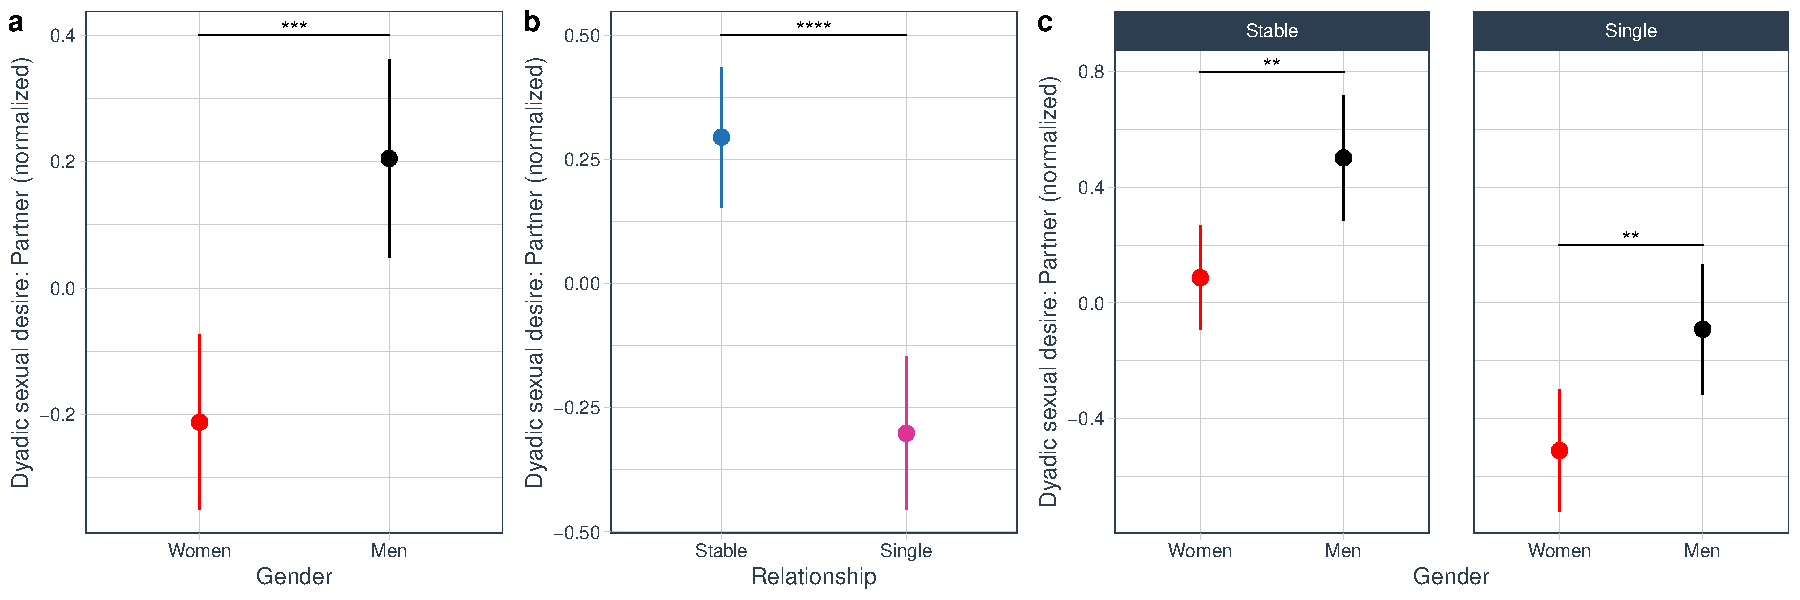
\includegraphics{Sexual_Desire_Arousal_V2_files/figure-latex/fig-h1c-1.pdf}
\caption{\label{fig:fig-h1c}Effects of gender and relationship type on Dyadic sexual desire: Partner. Dyadic sexual desire: Partner was transformed using ordered quantile normalization \autocite{petersonOrderedQuantileNormalization2020a}. \textbf{(a)} Simple comparison between sexual desire by gender (for detailed results, see Table \ref{tab:tab-m1c-emm1}); \textbf{(b)} Simple comparison between relationship status levels (for detailed results, see Table \ref{tab:tab-m1c-emm2}); \textbf{(c)} Interaction between relationship type and relationship status (see Table \ref{tab:tab-m1c}; for detailed results, see Table \ref{tab:tab-m1c-emm3}). White dots and black bars represent estimated marginal means and 95\% CI. In all cases, significant effects are represented with lines and stars: *\emph{p} \textless{} 0.05, **\emph{p} \textless{} 0.01, ***\emph{p} \textless{} 0.001, ****\emph{p} \textless{} 0.0001.}
\end{figure}

\subsection{Hypothesis 2: The association between trait sexual desire (TSD) and subjective sexual arousal (SSA) will vary by TSD dimension, with these associations being gender-specific in men and gender-non-specific in women.}\label{hyp2}

We tested whether the slope of SSA as predictor of sexual desire varies for each of the three dimensions of TSD (H1a: Solitary TSD; H1b: Dyadic TSD toward an attractive person; H1c: Dyadic TSD toward a partner), depending on the gender of the participants and the sex of the stimuli. The prediction was specific for each TSD dimension:

\begin{itemize}
\tightlist
\item
  \textbf{H2a}: A significant association between solitary TSD and SSA toward erotic stimuli.
\item
  \textbf{H2b}: A significant association between dyadic TSD toward an attractive person and SSA toward erotic stimuli.
\item
  \textbf{H2c}: No significant association between dyadic TSD toward a partner and SSA toward erotic stimuli.
\end{itemize}

To examine this hypothesis, we modeled the effects of SSA, gender, stimulus sex, and their interactions, on each of the three TSD scores. We included random intercepts for each stimuls, as well as random intercepts and slopes of stimuli sex for each participant.

However, models using the original TSD scores did not meet the assumption of normally distributed residuals. To address this, we applied an ordered normalization transformation to each TSD variable. We then fitted and compared models predicting both the original (as a proportion, to make scores comparable) and transformed (normalized) TSD dimensions. In all three cases, models using the normalized variables provided a better fit, so all inferences are based on these models.

\subsubsection{Data}\label{data-1}

A data frame was created with one row per participant, where sexual desire variables were normalized as proportions. An ordered quantile normalization transformation \autocite{petersonOrderedQuantileNormalization2020a} was then applied using the \texttt{orderNorm} function from the \texttt{bestNormalize} package \autocite{bestNormalizecit}, and the transformed values were added as new variables.

\begin{Shaded}
\begin{Highlighting}[]
\CommentTok{\# Process the dataset and create transformed variables  }
\NormalTok{dat\_m1 }\OtherTok{\textless{}{-}}\NormalTok{ dat }\SpecialCharTok{|\textgreater{}}  
  \CommentTok{\# Group the data by participant  }
  \FunctionTok{group\_by}\NormalTok{(Participant) }\SpecialCharTok{|\textgreater{}}  
  \CommentTok{\# Select only the first (top) observation for each participant  }
  \FunctionTok{slice\_head}\NormalTok{() }\SpecialCharTok{|\textgreater{}}  
  \CommentTok{\# Remove the grouping structure to avoid unintended behavior in later operations  }
  \FunctionTok{ungroup}\NormalTok{() }\SpecialCharTok{|\textgreater{}}  
  \CommentTok{\# Create new proportion variables by normalizing each sexual desire measure  }
  \FunctionTok{mutate}\NormalTok{(}\StringTok{"Solitary sexual desire (proportion)"} \OtherTok{=} 
           \StringTok{\textasciigrave{}}\AttributeTok{Solitary sexual desire}\StringTok{\textasciigrave{}} \SpecialCharTok{/} \DecValTok{31}\NormalTok{,  }
         \StringTok{"Dyadic sexual desire: Attractive person (proportion)"} \OtherTok{=} 
           \StringTok{\textasciigrave{}}\AttributeTok{Dyadic sexual desire (Attractive person)}\StringTok{\textasciigrave{}} \SpecialCharTok{/} \DecValTok{32}\NormalTok{,  }
         \StringTok{"Dyadic sexual desire: Partner (proportion)"} \OtherTok{=} 
           \StringTok{\textasciigrave{}}\AttributeTok{Dyadic sexual desire (Partner)}\StringTok{\textasciigrave{}} \SpecialCharTok{/} \DecValTok{38}\NormalTok{)  }

\CommentTok{\# Apply ordered normalization transformations to the proportion variables  }
\NormalTok{trs\_SSD }\OtherTok{\textless{}{-}} \FunctionTok{orderNorm}\NormalTok{(dat\_m1}\SpecialCharTok{$}\StringTok{\textasciigrave{}}\AttributeTok{Solitary sexual desire (proportion)}\StringTok{\textasciigrave{}}\NormalTok{)  }
\NormalTok{trs\_DSDat }\OtherTok{\textless{}{-}} \FunctionTok{orderNorm}\NormalTok{(dat\_m1}\SpecialCharTok{$}\StringTok{\textasciigrave{}}\AttributeTok{Dyadic sexual desire: Attractive person (proportion)}\StringTok{\textasciigrave{}}\NormalTok{)  }
\NormalTok{trs\_DSDpt }\OtherTok{\textless{}{-}} \FunctionTok{orderNorm}\NormalTok{(dat\_m1}\SpecialCharTok{$}\StringTok{\textasciigrave{}}\AttributeTok{Dyadic sexual desire: Partner (proportion)}\StringTok{\textasciigrave{}}\NormalTok{)  }

\CommentTok{\# Add the transformed variables back into the dataset  }
\NormalTok{dat\_m1 }\OtherTok{\textless{}{-}}\NormalTok{ dat\_m1 }\SpecialCharTok{|\textgreater{}}  
  \FunctionTok{mutate}\NormalTok{(}\StringTok{"Solitary sexual desire (normalized)"} \OtherTok{=} 
           \FunctionTok{predict}\NormalTok{(trs\_SSD),  }\CommentTok{\# Transformed solitary sexual desire  }
         \StringTok{"Dyadic sexual desire: Attractive person (normalized)"} \OtherTok{=} 
           \FunctionTok{predict}\NormalTok{(trs\_DSDat),  }\CommentTok{\# Transformed dyadic sexual desire (attractive person)  }
         \StringTok{"Dyadic sexual desire: Partner (normalized)"} \OtherTok{=} 
           \FunctionTok{predict}\NormalTok{(trs\_DSDpt))  }\CommentTok{\# Transformed dyadic sexual desire (partner)  }
\end{Highlighting}
\end{Shaded}

\subsubsection{Hypothesis 1a: Solitary TSD}\label{hypothesis1a}

\paragraph{Model the effects of relationship type and gender on Solitary TSD}\label{model-the-effects-of-relationship-type-and-gender-on-solitary-tsd-3}

We fitted models with both the original (proportion; \texttt{m1a\_prop}) and transformed (normalized; \texttt{m1a\_norm}) TSD scores, and performed posterior predictive checks (PPCs). As shown elsewhere \autocite[e.g.,][]{gabryVisualizationBayesianWorkflow2019}, if simulated data from one model are more similar to the observed outcome, that model is likely to be preferred.

\begin{Shaded}
\begin{Highlighting}[]
\FunctionTok{options}\NormalTok{(}\AttributeTok{contrasts =} \FunctionTok{c}\NormalTok{(}\StringTok{"contr.sum"}\NormalTok{,}\StringTok{"contr.poly"}\NormalTok{))}
\NormalTok{m1a\_prop }\OtherTok{\textless{}{-}} \FunctionTok{lm}\NormalTok{(}\StringTok{\textasciigrave{}}\AttributeTok{Solitary sexual desire (proportion)}\StringTok{\textasciigrave{}} \SpecialCharTok{\textasciitilde{}}\NormalTok{ Gender }\SpecialCharTok{*}\NormalTok{ Relationship,}
            \AttributeTok{data =}\NormalTok{ dat\_m1)}

\NormalTok{m1a\_norm }\OtherTok{\textless{}{-}} \FunctionTok{lm}\NormalTok{(}\StringTok{\textasciigrave{}}\AttributeTok{Solitary sexual desire (normalized)}\StringTok{\textasciigrave{}} \SpecialCharTok{\textasciitilde{}}\NormalTok{ Gender }\SpecialCharTok{*}\NormalTok{ Relationship,}
           \AttributeTok{data =}\NormalTok{ dat\_m1)}
\end{Highlighting}
\end{Shaded}

\subparagraph{Figure \ref{fig:ppc-m1a}: Posterior predictive checks (PPCs) for Hypothesis 1a.}\label{figure-reffigppc-m1a-posterior-predictive-checks-ppcs-for-hypothesis-1a.-1}

PPCs were performed using the \texttt{check\_model} function from the \texttt{performance} package \autocite{ludecke2021}, and reported in Fig. \ref{fig:ppc-m1a}. Simulated data from the normalized Solitary TSD model (Fig. \ref{fig:ppc-m1a}b) are more similar to the observed outcome, so this model is preferred.

\begin{Shaded}
\begin{Highlighting}[]
\NormalTok{ppc\_m2a }\OtherTok{\textless{}{-}} \FunctionTok{ggarrange}\NormalTok{(}\FunctionTok{plot}\NormalTok{(}\FunctionTok{check\_model}\NormalTok{(m1a\_prop, }
                                      \AttributeTok{panel =} \ConstantTok{FALSE}\NormalTok{,}
                                      \AttributeTok{check =} \StringTok{"pp\_check"}\NormalTok{)}\SpecialCharTok{$}\NormalTok{PP\_CHECK,}
                          \AttributeTok{colors =} \FunctionTok{c}\NormalTok{(}\StringTok{"red"}\NormalTok{, }\StringTok{"grey30"}\NormalTok{)) }\SpecialCharTok{+}
                       \FunctionTok{labs}\NormalTok{(}\AttributeTok{title =} \ConstantTok{NULL}\NormalTok{, }\AttributeTok{subtitle =} \ConstantTok{NULL}\NormalTok{) }\SpecialCharTok{+}
                       \FunctionTok{theme\_tq}\NormalTok{() }\SpecialCharTok{+}
                       \FunctionTok{facet\_wrap}\NormalTok{(}\SpecialCharTok{\textasciitilde{}} \DecValTok{1}\NormalTok{, }\AttributeTok{labeller =} \FunctionTok{as\_labeller}\NormalTok{(}\FunctionTok{c}\NormalTok{(}
                         \StringTok{"1"} \OtherTok{=} \StringTok{"Original (proportion) Solitary TSD"}\NormalTok{))),}
                     \FunctionTok{plot}\NormalTok{(}\FunctionTok{check\_model}\NormalTok{(m1a\_norm, }
                                      \AttributeTok{panel =} \ConstantTok{FALSE}\NormalTok{,}
                                      \AttributeTok{check =} \StringTok{"pp\_check"}\NormalTok{)}\SpecialCharTok{$}\NormalTok{PP\_CHECK,}
                          \AttributeTok{colors =} \FunctionTok{c}\NormalTok{(}\StringTok{"red"}\NormalTok{, }\StringTok{"grey30"}\NormalTok{)) }\SpecialCharTok{+}
                       \FunctionTok{labs}\NormalTok{(}\AttributeTok{title =} \ConstantTok{NULL}\NormalTok{, }\AttributeTok{subtitle =} \ConstantTok{NULL}\NormalTok{) }\SpecialCharTok{+}
                       \FunctionTok{theme\_tq}\NormalTok{() }\SpecialCharTok{+}
                       \FunctionTok{facet\_wrap}\NormalTok{(}\SpecialCharTok{\textasciitilde{}} \DecValTok{1}\NormalTok{, }\AttributeTok{labeller =} \FunctionTok{as\_labeller}\NormalTok{(}\FunctionTok{c}\NormalTok{(}
                         \StringTok{"1"} \OtherTok{=} \StringTok{"Transformed (normalized) Solitary TSD"}\NormalTok{))),}
                     \AttributeTok{labels =} \StringTok{"auto"}\NormalTok{,}
                     \AttributeTok{common.legend =} \ConstantTok{TRUE}\NormalTok{,}
                     \AttributeTok{legend =} \StringTok{"bottom"}\NormalTok{)}
\NormalTok{ppc\_m1a}
\end{Highlighting}
\end{Shaded}

\begin{figure}
\centering
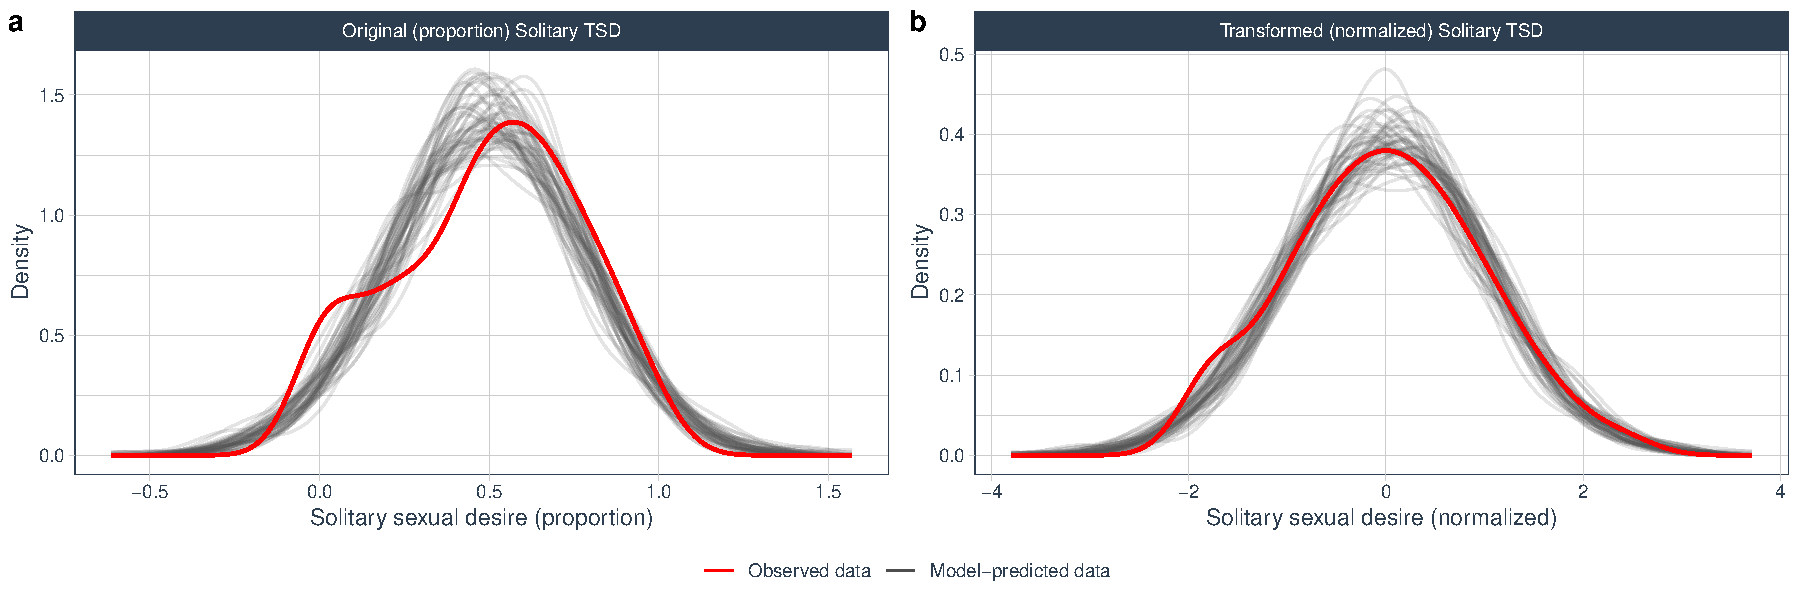
\includegraphics{Sexual_Desire_Arousal_V2_files/figure-latex/ppc-m2a-1.pdf}
\caption{\label{fig:ppc-m2a}Posterior predictive check. \textbf{(a)} Original (proportion) Solitary TSD; \textbf{(b)} Transformed (normalized) Solitary TSD. In both panels, red lines represent the observed data, and thin black lines represent 50 iterations of simulated data from each model.}
\end{figure}

\begin{center}\rule{0.5\linewidth}{0.5pt}\end{center}

\section{Session info (for reproducibility)}\label{session}

\begin{Shaded}
\begin{Highlighting}[]
\FunctionTok{library}\NormalTok{(pander)}
\FunctionTok{pander}\NormalTok{(}\FunctionTok{sessionInfo}\NormalTok{(), }\AttributeTok{locale =} \ConstantTok{FALSE}\NormalTok{)}
\end{Highlighting}
\end{Shaded}

\textbf{R version 4.4.2 (2024-10-31)}

\textbf{Platform:} x86\_64-pc-linux-gnu

\textbf{attached base packages:}
\emph{stats}, \emph{graphics}, \emph{grDevices}, \emph{utils}, \emph{datasets}, \emph{methods} and \emph{base}

\textbf{other attached packages:}
\emph{pander(v.0.6.5)}, \emph{Hmisc(v.5.2-2)}, \emph{rstatix(v.0.7.2)}, \emph{bestNormalize(v.1.9.1)}, \emph{berryFunctions(v.1.22.5)}, \emph{emmeans(v.1.10.7)}, \emph{lmerTest(v.3.1-3)}, \emph{lme4(v.1.1-36)}, \emph{Matrix(v.1.7-2)}, \emph{scales(v.1.3.0)}, \emph{psych(v.2.4.12)}, \emph{kableExtra(v.1.4.0)}, \emph{performance(v.0.13.0)}, \emph{PerformanceAnalytics(v.2.0.8)}, \emph{quantmod(v.0.4.26)}, \emph{TTR(v.0.24.4)}, \emph{xts(v.0.14.1)}, \emph{zoo(v.1.8-12)}, \emph{tidyquant(v.1.0.10)}, \emph{ggpubr(v.0.6.0)}, \emph{lubridate(v.1.9.4)}, \emph{forcats(v.1.0.0)}, \emph{stringr(v.1.5.1)}, \emph{dplyr(v.1.1.4)}, \emph{purrr(v.1.0.4)}, \emph{readr(v.2.1.5)}, \emph{tidyr(v.1.3.1)}, \emph{tibble(v.3.2.1)}, \emph{ggplot2(v.3.5.1)}, \emph{tidyverse(v.2.0.0)}, \emph{car(v.3.1-3)}, \emph{carData(v.3.0-5)}, \emph{ltm(v.1.2-0)}, \emph{polycor(v.0.8-1)}, \emph{msm(v.1.8.2)}, \emph{MASS(v.7.3-64)}, \emph{readxl(v.1.4.3)} and \emph{knitr(v.1.49)}

\textbf{loaded via a namespace (and not attached):}
\emph{rstudioapi(v.0.17.1)}, \emph{magrittr(v.2.0.3)}, \emph{TH.data(v.1.1-3)}, \emph{estimability(v.1.5.1)}, \emph{farver(v.2.1.2)}, \emph{nloptr(v.2.1.1)}, \emph{rmarkdown(v.2.29)}, \emph{vctrs(v.0.6.5)}, \emph{minqa(v.1.2.8)}, \emph{base64enc(v.0.1-3)}, \emph{butcher(v.0.3.4)}, \emph{htmltools(v.0.5.8.1)}, \emph{curl(v.6.2.0)}, \emph{broom(v.1.0.7)}, \emph{cellranger(v.1.1.0)}, \emph{Formula(v.1.2-5)}, \emph{parallelly(v.1.42.0)}, \emph{htmlwidgets(v.1.6.4)}, \emph{sandwich(v.3.1-1)}, \emph{admisc(v.0.37)}, \emph{lifecycle(v.1.0.4)}, \emph{iterators(v.1.0.14)}, \emph{pkgconfig(v.2.0.3)}, \emph{R6(v.2.5.1)}, \emph{fastmap(v.1.2.0)}, \emph{rbibutils(v.2.3)}, \emph{future(v.1.34.0)}, \emph{digest(v.0.6.37)}, \emph{numDeriv(v.2016.8-1.1)}, \emph{colorspace(v.2.1-1)}, \emph{labeling(v.0.4.3)}, \emph{timechange(v.0.3.0)}, \emph{abind(v.1.4-8)}, \emph{compiler(v.4.4.2)}, \emph{rngtools(v.1.5.2)}, \emph{withr(v.3.0.2)}, \emph{doParallel(v.1.0.17)}, \emph{htmlTable(v.2.4.3)}, \emph{backports(v.1.5.0)}, \emph{ggsignif(v.0.6.4)}, \emph{lava(v.1.8.1)}, \emph{tools(v.4.4.2)}, \emph{foreign(v.0.8-88)}, \emph{RobStatTM(v.1.0.11)}, \emph{future.apply(v.1.11.3)}, \emph{nnet(v.7.3-20)}, \emph{glue(v.1.8.0)}, \emph{quadprog(v.1.5-8)}, \emph{nlme(v.3.1-167)}, \emph{grid(v.4.4.2)}, \emph{checkmate(v.2.3.2)}, \emph{cluster(v.2.1.8)}, \emph{see(v.0.10.0)}, \emph{generics(v.0.1.3)}, \emph{recipes(v.1.1.0)}, \emph{gtable(v.0.3.6)}, \emph{nortest(v.1.0-4)}, \emph{tzdb(v.0.4.0)}, \emph{class(v.7.3-23)}, \emph{data.table(v.1.16.4)}, \emph{hms(v.1.1.3)}, \emph{xml2(v.1.3.6)}, \emph{foreach(v.1.5.2)}, \emph{pillar(v.1.10.1)}, \emph{splines(v.4.4.2)}, \emph{lattice(v.0.22-6)}, \emph{survival(v.3.8-3)}, \emph{tidyselect(v.1.2.1)}, \emph{gridExtra(v.2.3)}, \emph{reformulas(v.0.4.0)}, \emph{bookdown(v.0.42)}, \emph{svglite(v.2.1.3)}, \emph{xfun(v.0.50)}, \emph{expm(v.1.0-0)}, \emph{hardhat(v.1.4.1)}, \emph{timeDate(v.4041.110)}, \emph{stringi(v.1.8.4)}, \emph{yaml(v.2.3.10)}, \emph{boot(v.1.3-31)}, \emph{evaluate(v.1.0.3)}, \emph{codetools(v.0.2-20)}, \emph{cli(v.3.6.3)}, \emph{rpart(v.4.1.24)}, \emph{xtable(v.1.8-4)}, \emph{systemfonts(v.1.2.1)}, \emph{Rdpack(v.2.6.2)}, \emph{munsell(v.0.5.1)}, \emph{Rcpp(v.1.0.14)}, \emph{globals(v.0.16.3)}, \emph{coda(v.0.19-4.1)}, \emph{parallel(v.4.4.2)}, \emph{gower(v.1.0.2)}, \emph{doRNG(v.1.8.6.1)}, \emph{listenv(v.0.9.1)}, \emph{viridisLite(v.0.4.2)}, \emph{mvtnorm(v.1.3-3)}, \emph{ipred(v.0.9-15)}, \emph{prodlim(v.2024.06.25)}, \emph{insight(v.1.0.2)}, \emph{rlang(v.1.1.5)}, \emph{cowplot(v.1.1.3)}, \emph{multcomp(v.1.4-28)} and \emph{mnormt(v.2.1.1)}

\begin{center}\rule{0.5\linewidth}{0.5pt}\end{center}

\section{Supplementary references}\label{refs}

\begin{multicols}{2}
\AtNextBibliography{\footnotesize}
\printbibliography[heading=none]
\normalsize
\end{multicols}

\def\printbibliography{}

\printbibliography

\end{document}
